\begin{figure}[H]
\centering
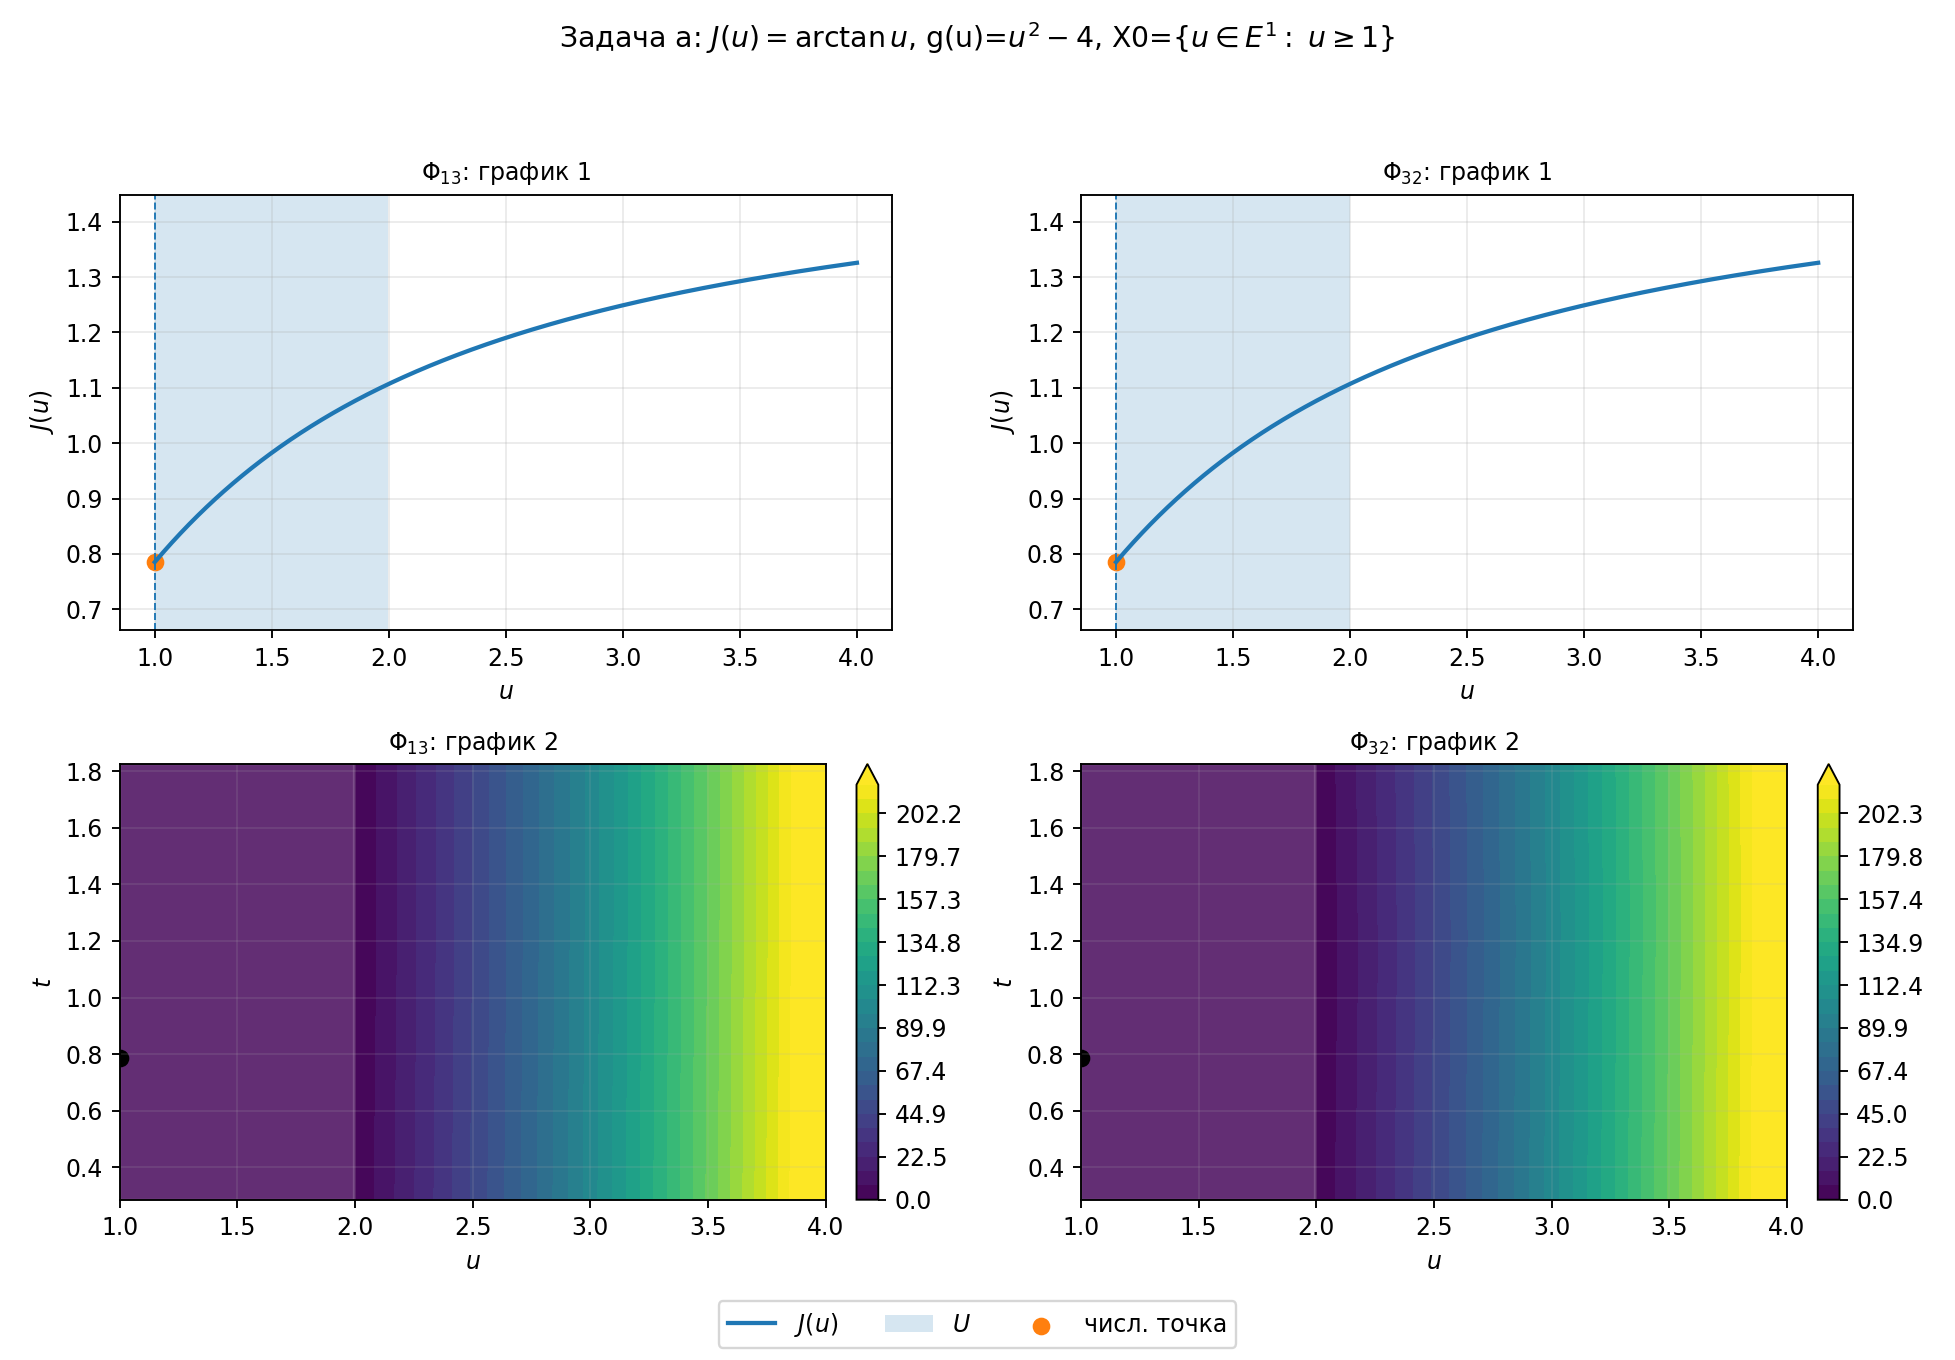
\includegraphics[width=0.96\textwidth]{graphs/a_g1_xge1_overview.png}
\caption{Задача а, вариант g1: $g(u)=u^2-4$, $X_0=\{u\in E^1:\ u\geq 1\}$. Верхний ряд: график 1 для $\Phi_{13}$ и $\Phi_{32}$; нижний ряд: график 2 для $\Phi_{13}$ и $\Phi_{32}$.}
\end{figure}

\begin{figure}[H]
\centering
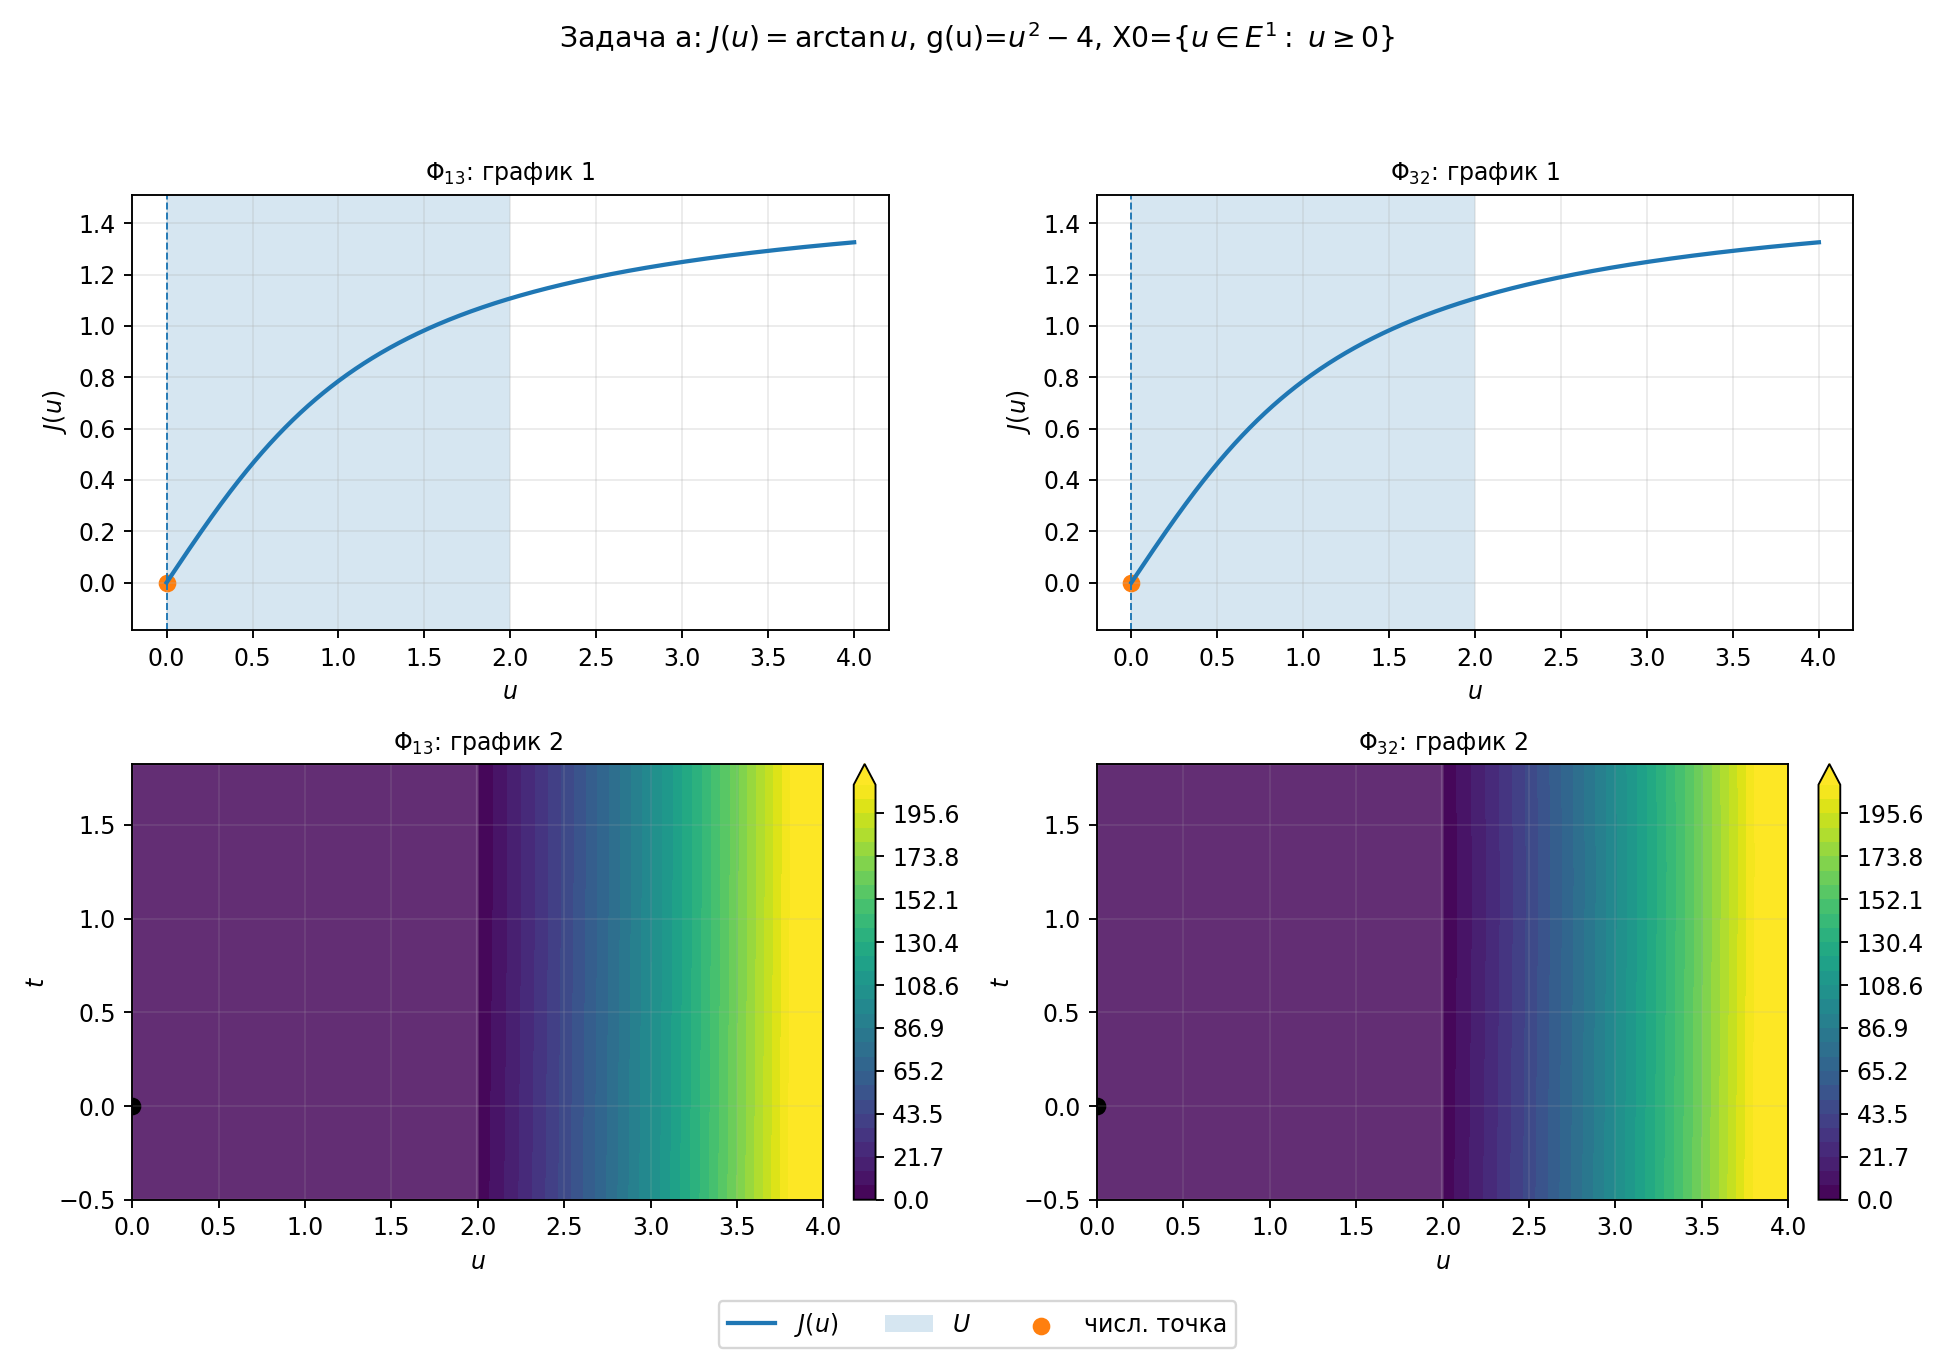
\includegraphics[width=0.96\textwidth]{graphs/a_g1_xge0_overview.png}
\caption{Задача а, вариант g1: $g(u)=u^2-4$, $X_0=\{u\in E^1:\ u\geq 0\}$. Верхний ряд: график 1 для $\Phi_{13}$ и $\Phi_{32}$; нижний ряд: график 2 для $\Phi_{13}$ и $\Phi_{32}$.}
\end{figure}

\begin{figure}[H]
\centering
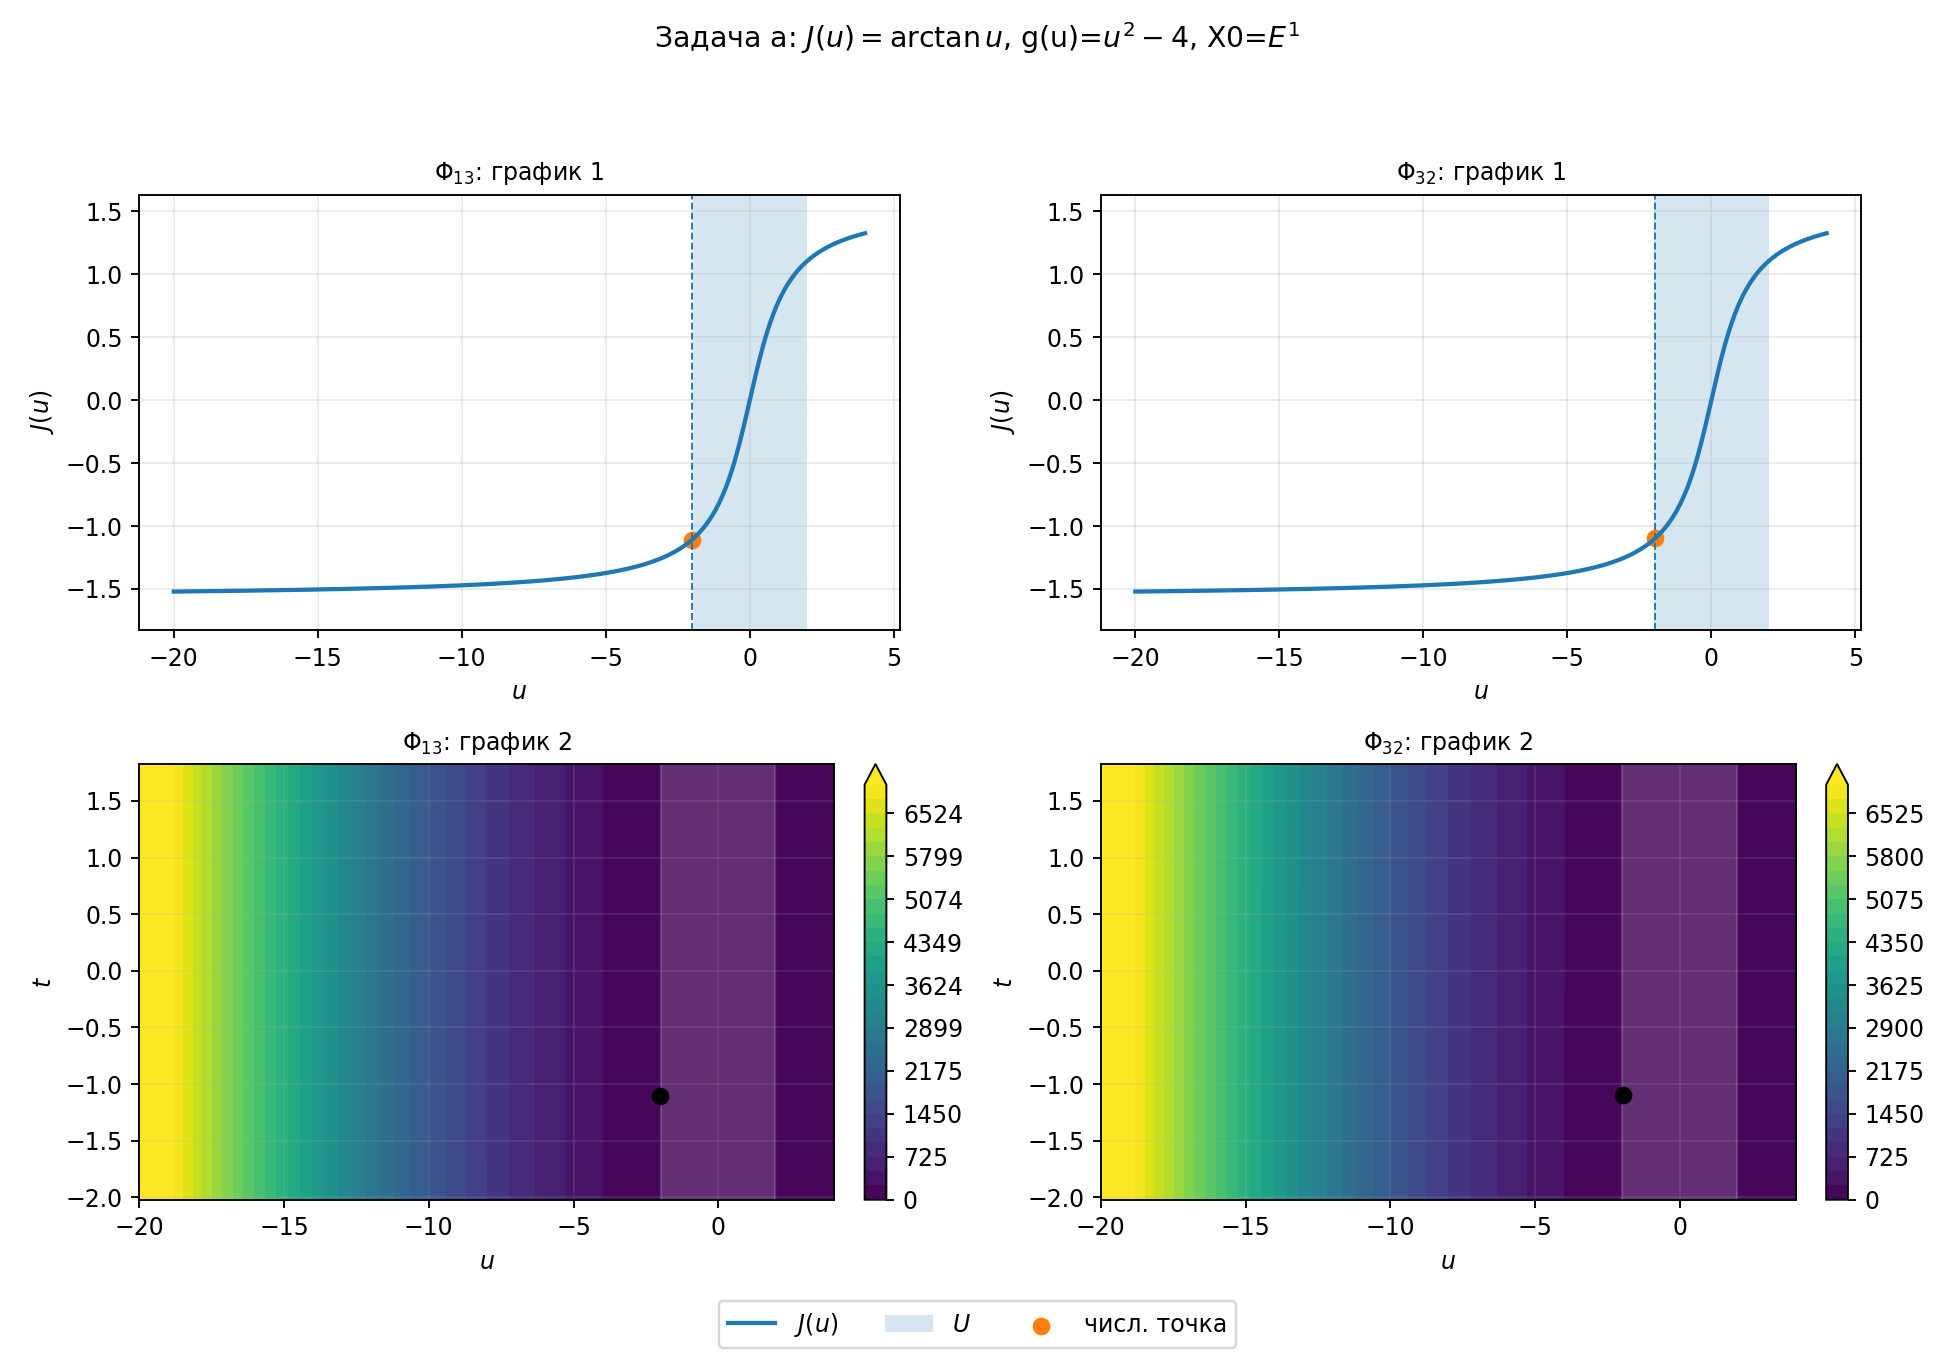
\includegraphics[width=0.96\textwidth]{graphs/a_g1_R_overview.png}
\caption{Задача а, вариант g1: $g(u)=u^2-4$, $X_0=E^1$. Верхний ряд: график 1 для $\Phi_{13}$ и $\Phi_{32}$; нижний ряд: график 2 для $\Phi_{13}$ и $\Phi_{32}$.}
\end{figure}

\begin{figure}[H]
\centering
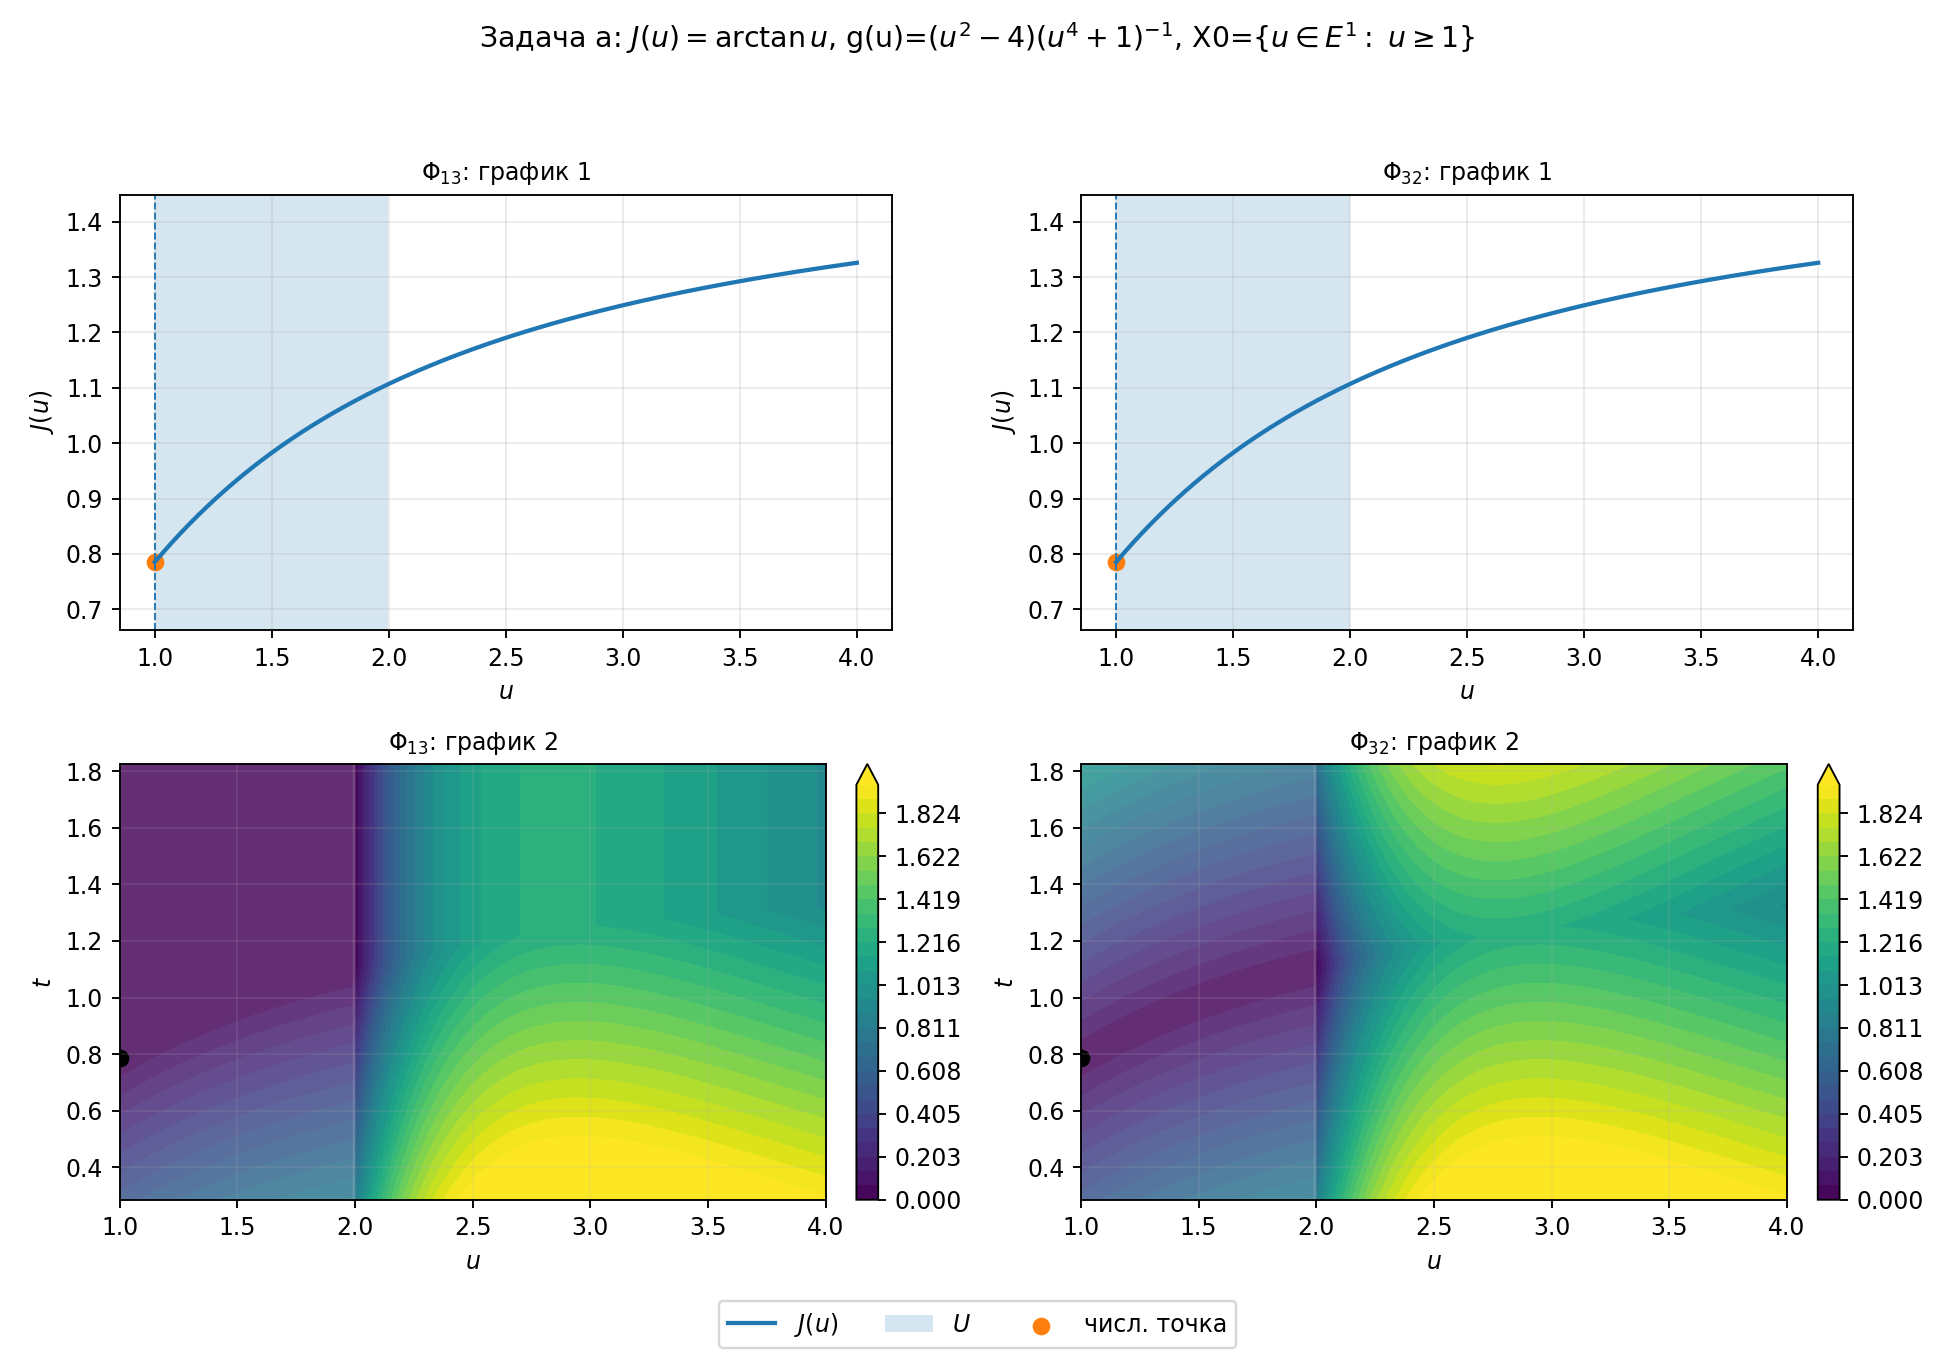
\includegraphics[width=0.96\textwidth]{graphs/a_g2_xge1_overview.png}
\caption{Задача а, вариант g2: $g(u)=(u^2-4)(u^4+1)^{-1}$, $X_0=\{u\in E^1:\ u\geq 1\}$. Верхний ряд: график 1 для $\Phi_{13}$ и $\Phi_{32}$; нижний ряд: график 2 для $\Phi_{13}$ и $\Phi_{32}$.}
\end{figure}

\begin{figure}[H]
\centering
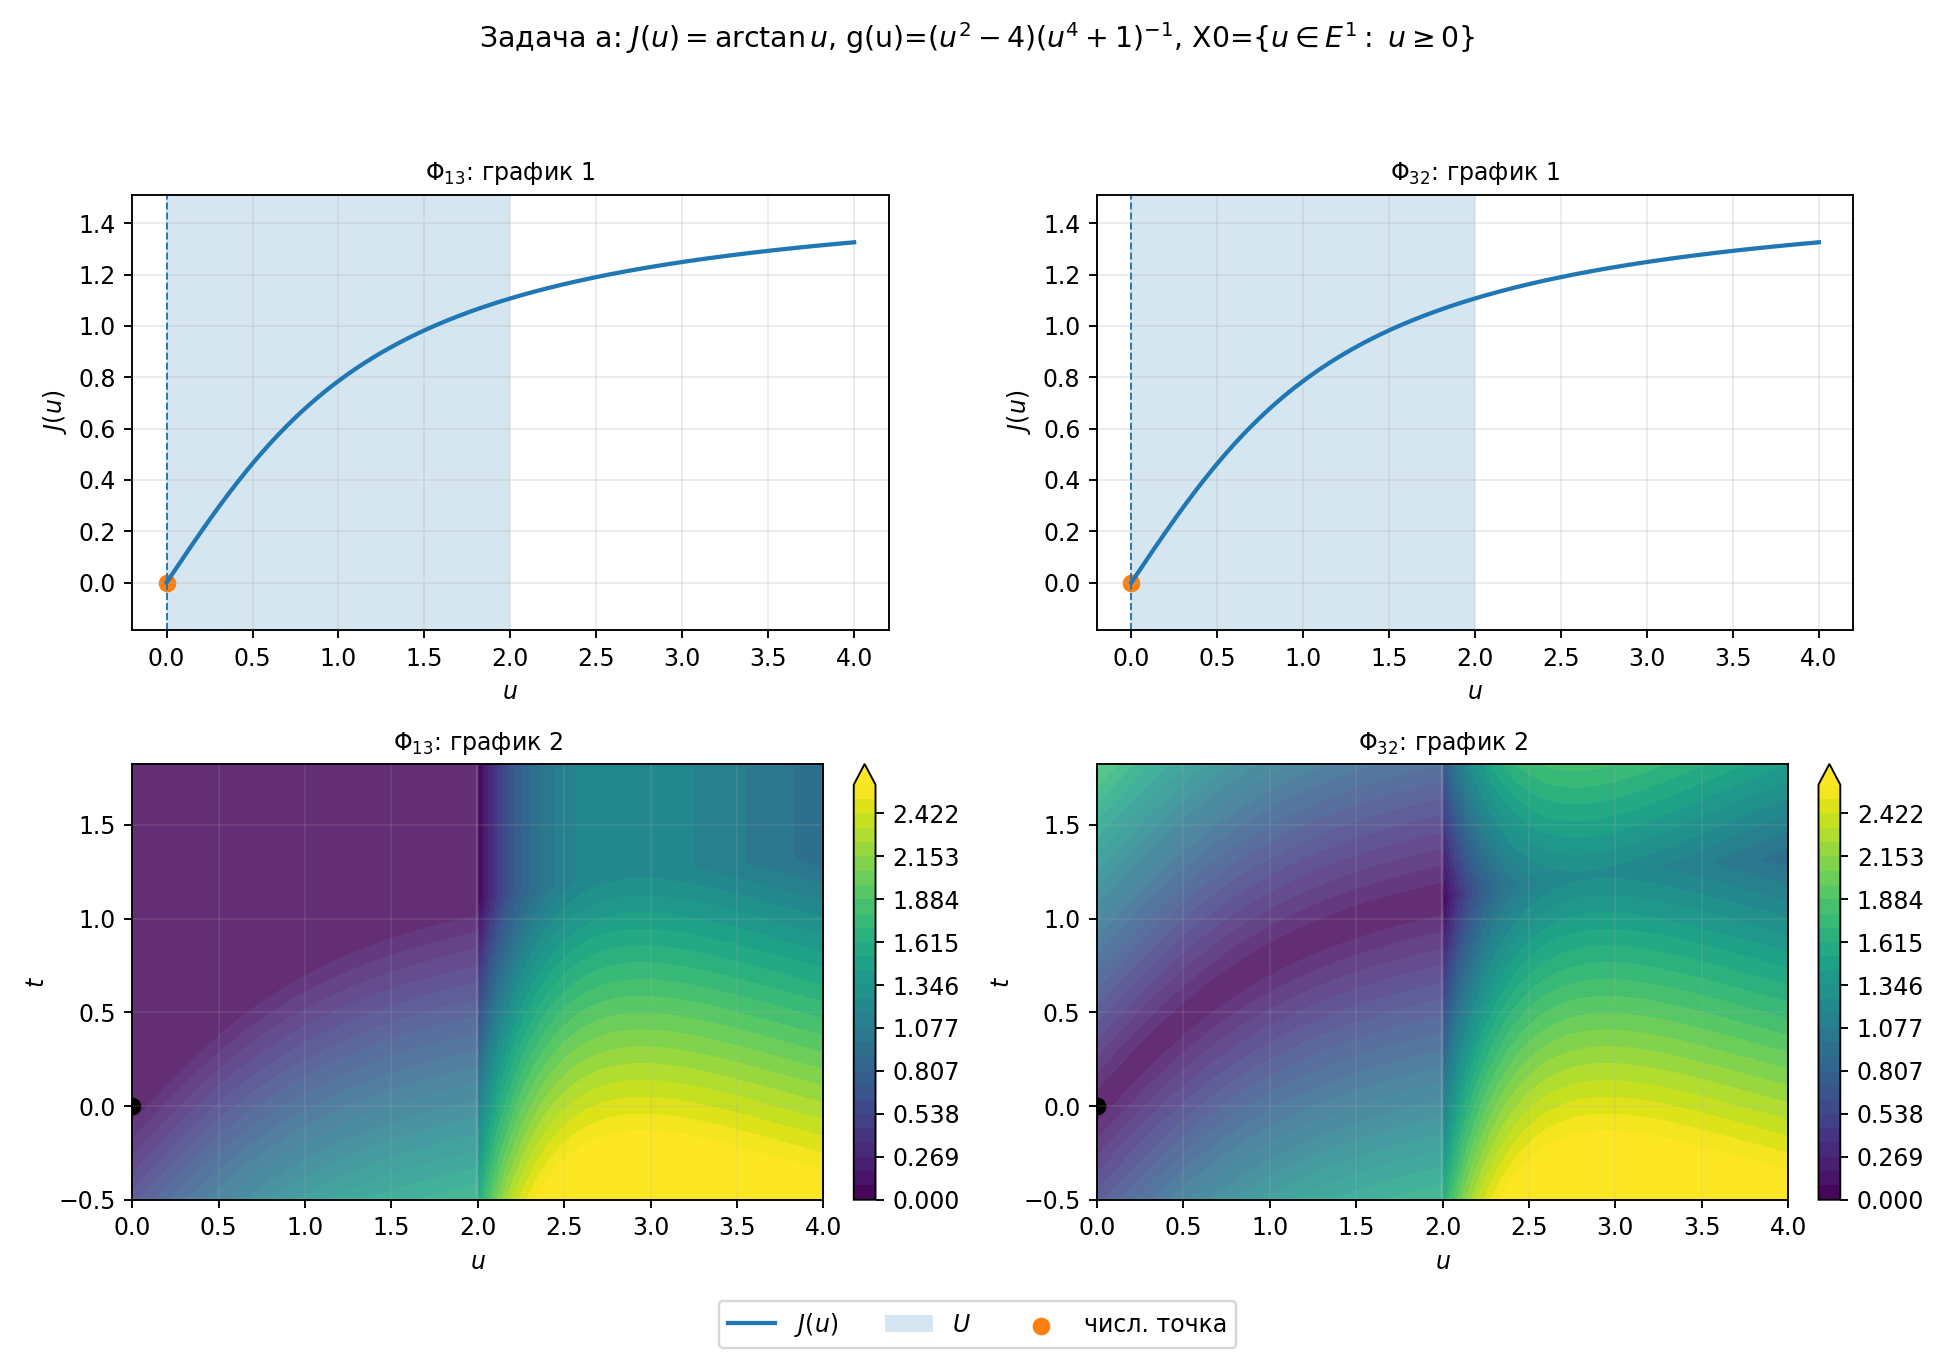
\includegraphics[width=0.96\textwidth]{graphs/a_g2_xge0_overview.png}
\caption{Задача а, вариант g2: $g(u)=(u^2-4)(u^4+1)^{-1}$, $X_0=\{u\in E^1:\ u\geq 0\}$. Верхний ряд: график 1 для $\Phi_{13}$ и $\Phi_{32}$; нижний ряд: график 2 для $\Phi_{13}$ и $\Phi_{32}$.}
\end{figure}

\begin{figure}[H]
\centering
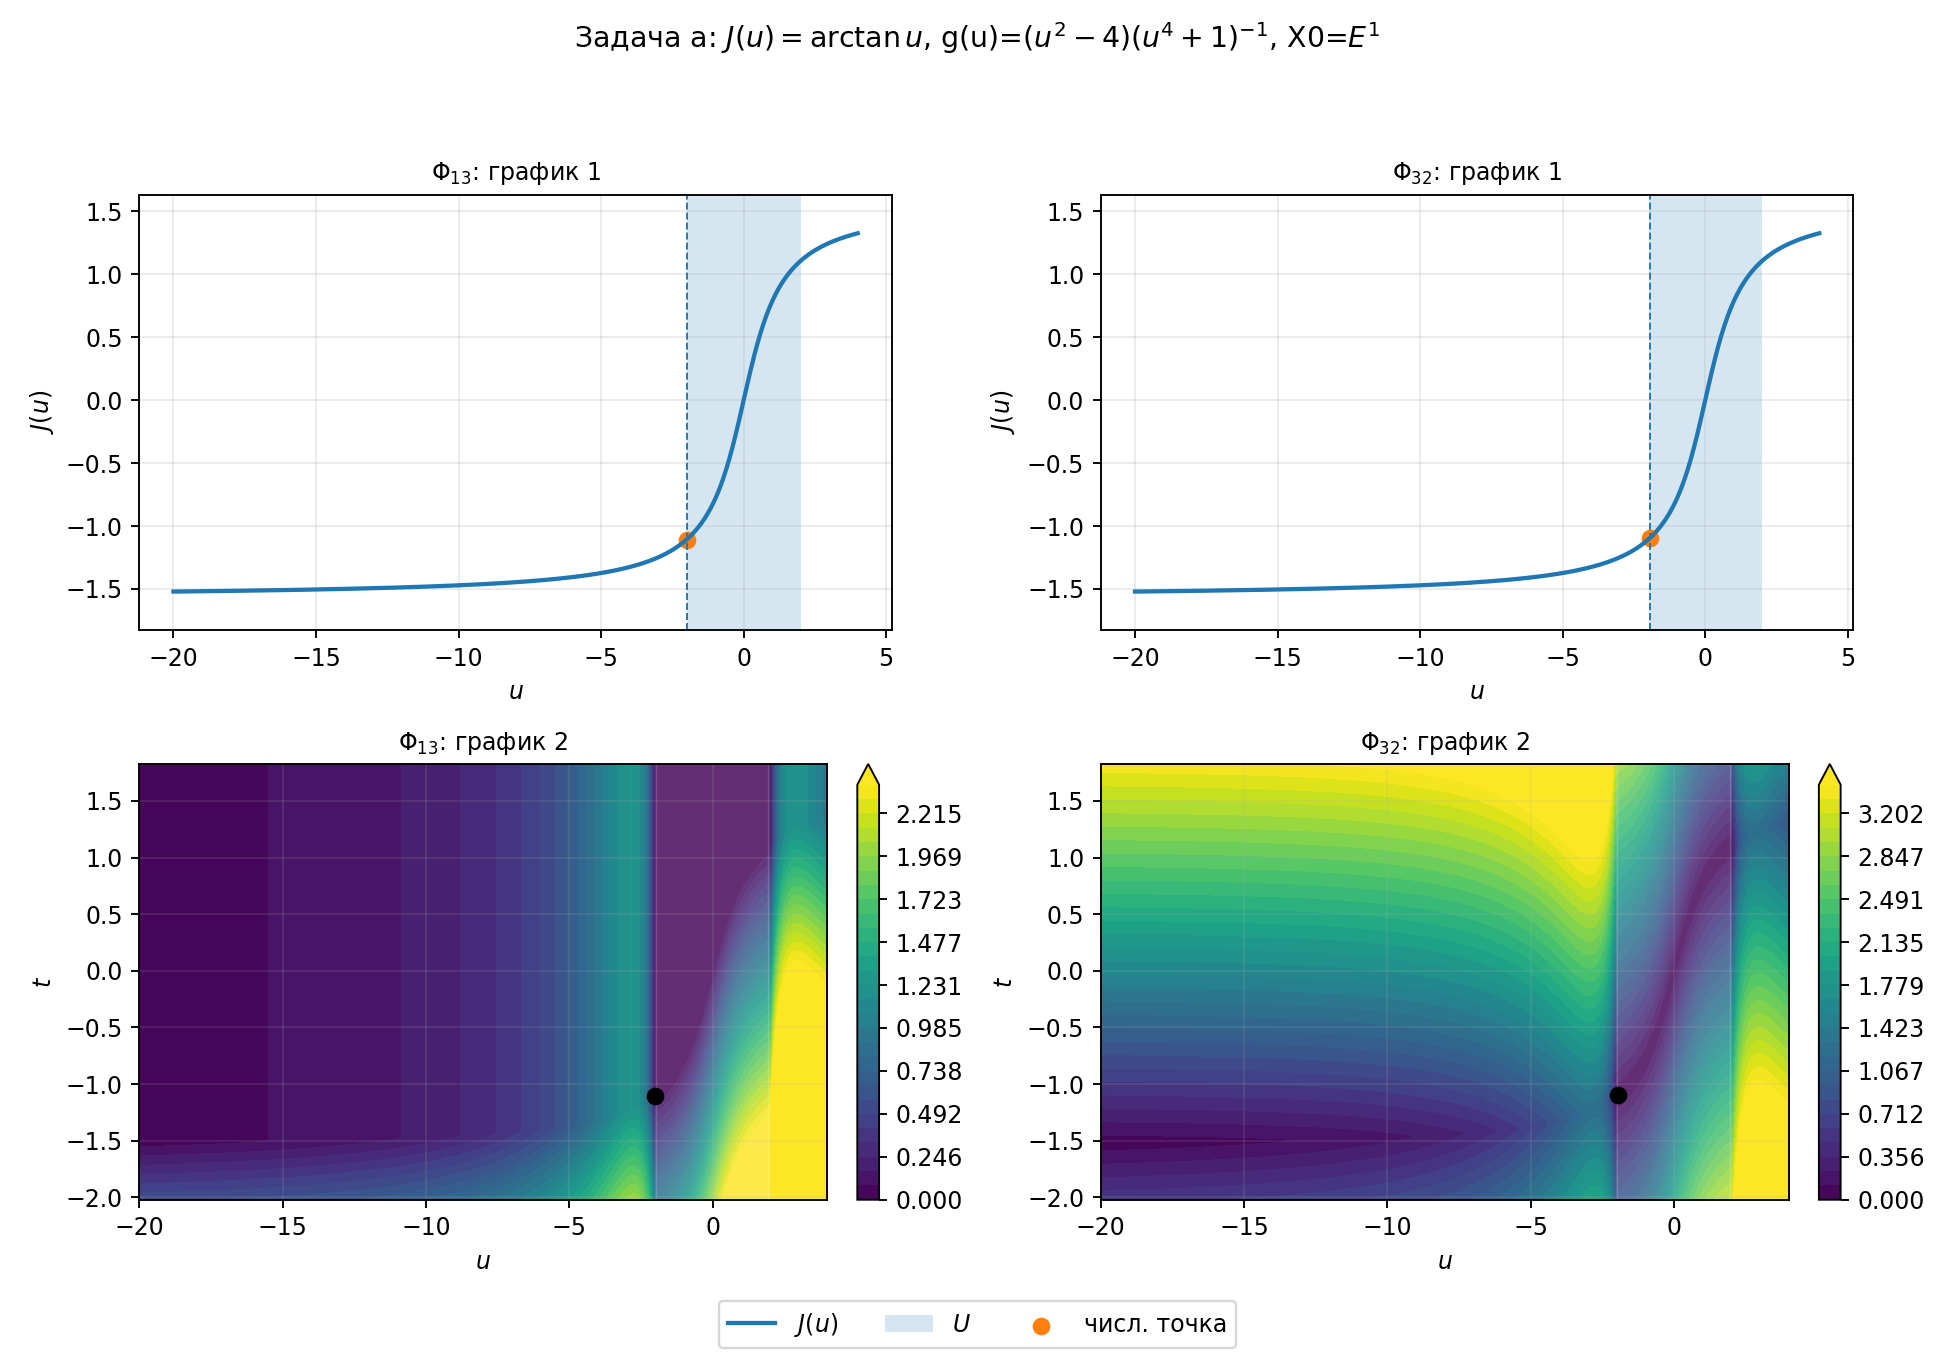
\includegraphics[width=0.96\textwidth]{graphs/a_g2_R_overview.png}
\caption{Задача а, вариант g2: $g(u)=(u^2-4)(u^4+1)^{-1}$, $X_0=E^1$. Верхний ряд: график 1 для $\Phi_{13}$ и $\Phi_{32}$; нижний ряд: график 2 для $\Phi_{13}$ и $\Phi_{32}$.}
\end{figure}

\begin{figure}[H]
\centering
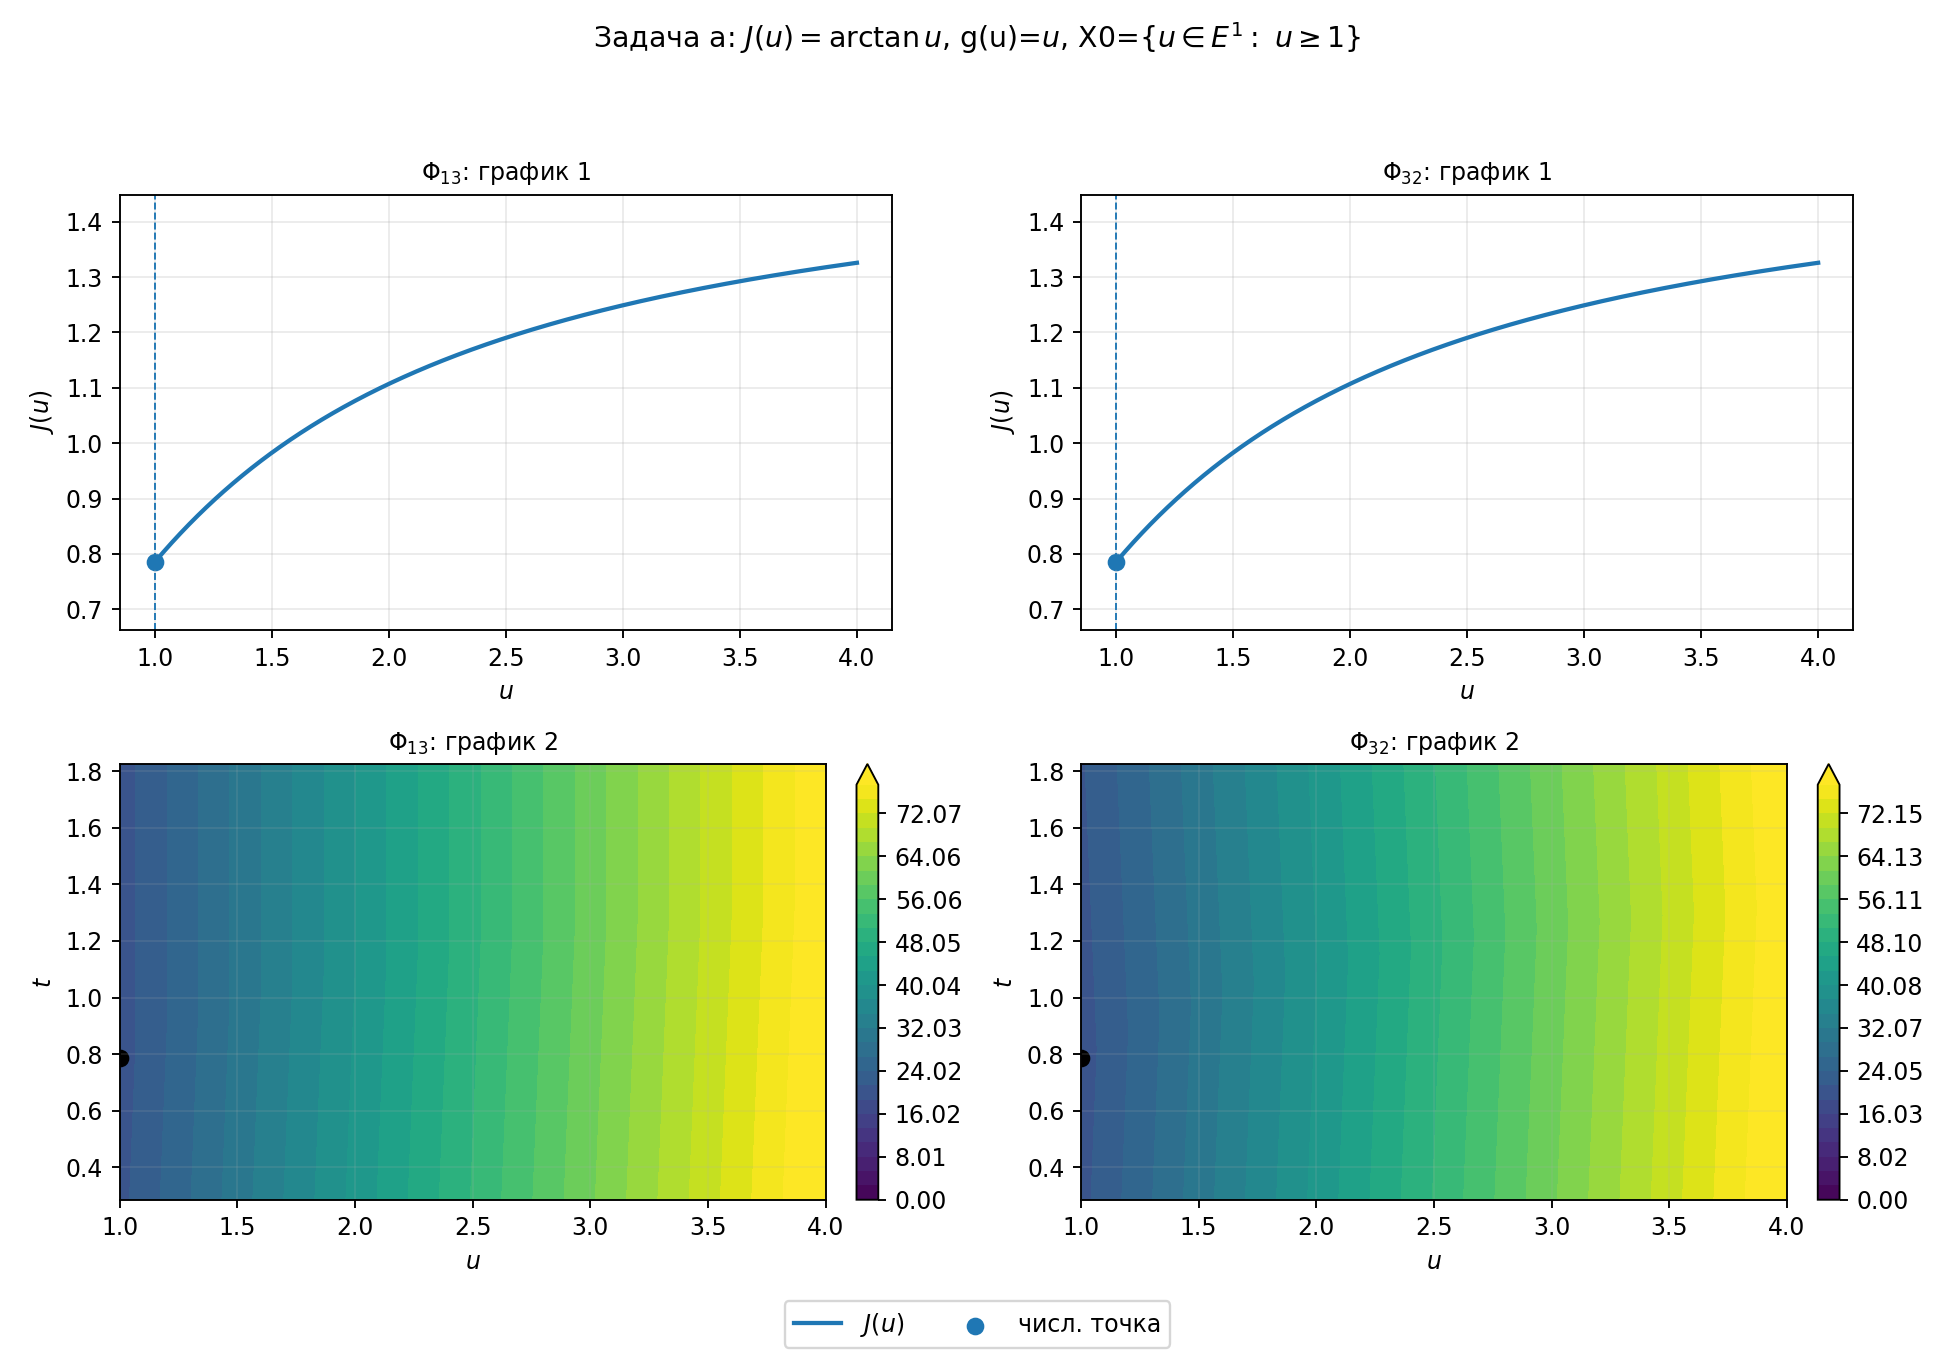
\includegraphics[width=0.96\textwidth]{graphs/a_g3_xge1_overview.png}
\caption{Задача а, вариант g3: $g(u)=u$, $X_0=\{u\in E^1:\ u\geq 1\}$. Верхний ряд: график 1 для $\Phi_{13}$ и $\Phi_{32}$; нижний ряд: график 2 для $\Phi_{13}$ и $\Phi_{32}$.}
\end{figure}

\begin{figure}[H]
\centering
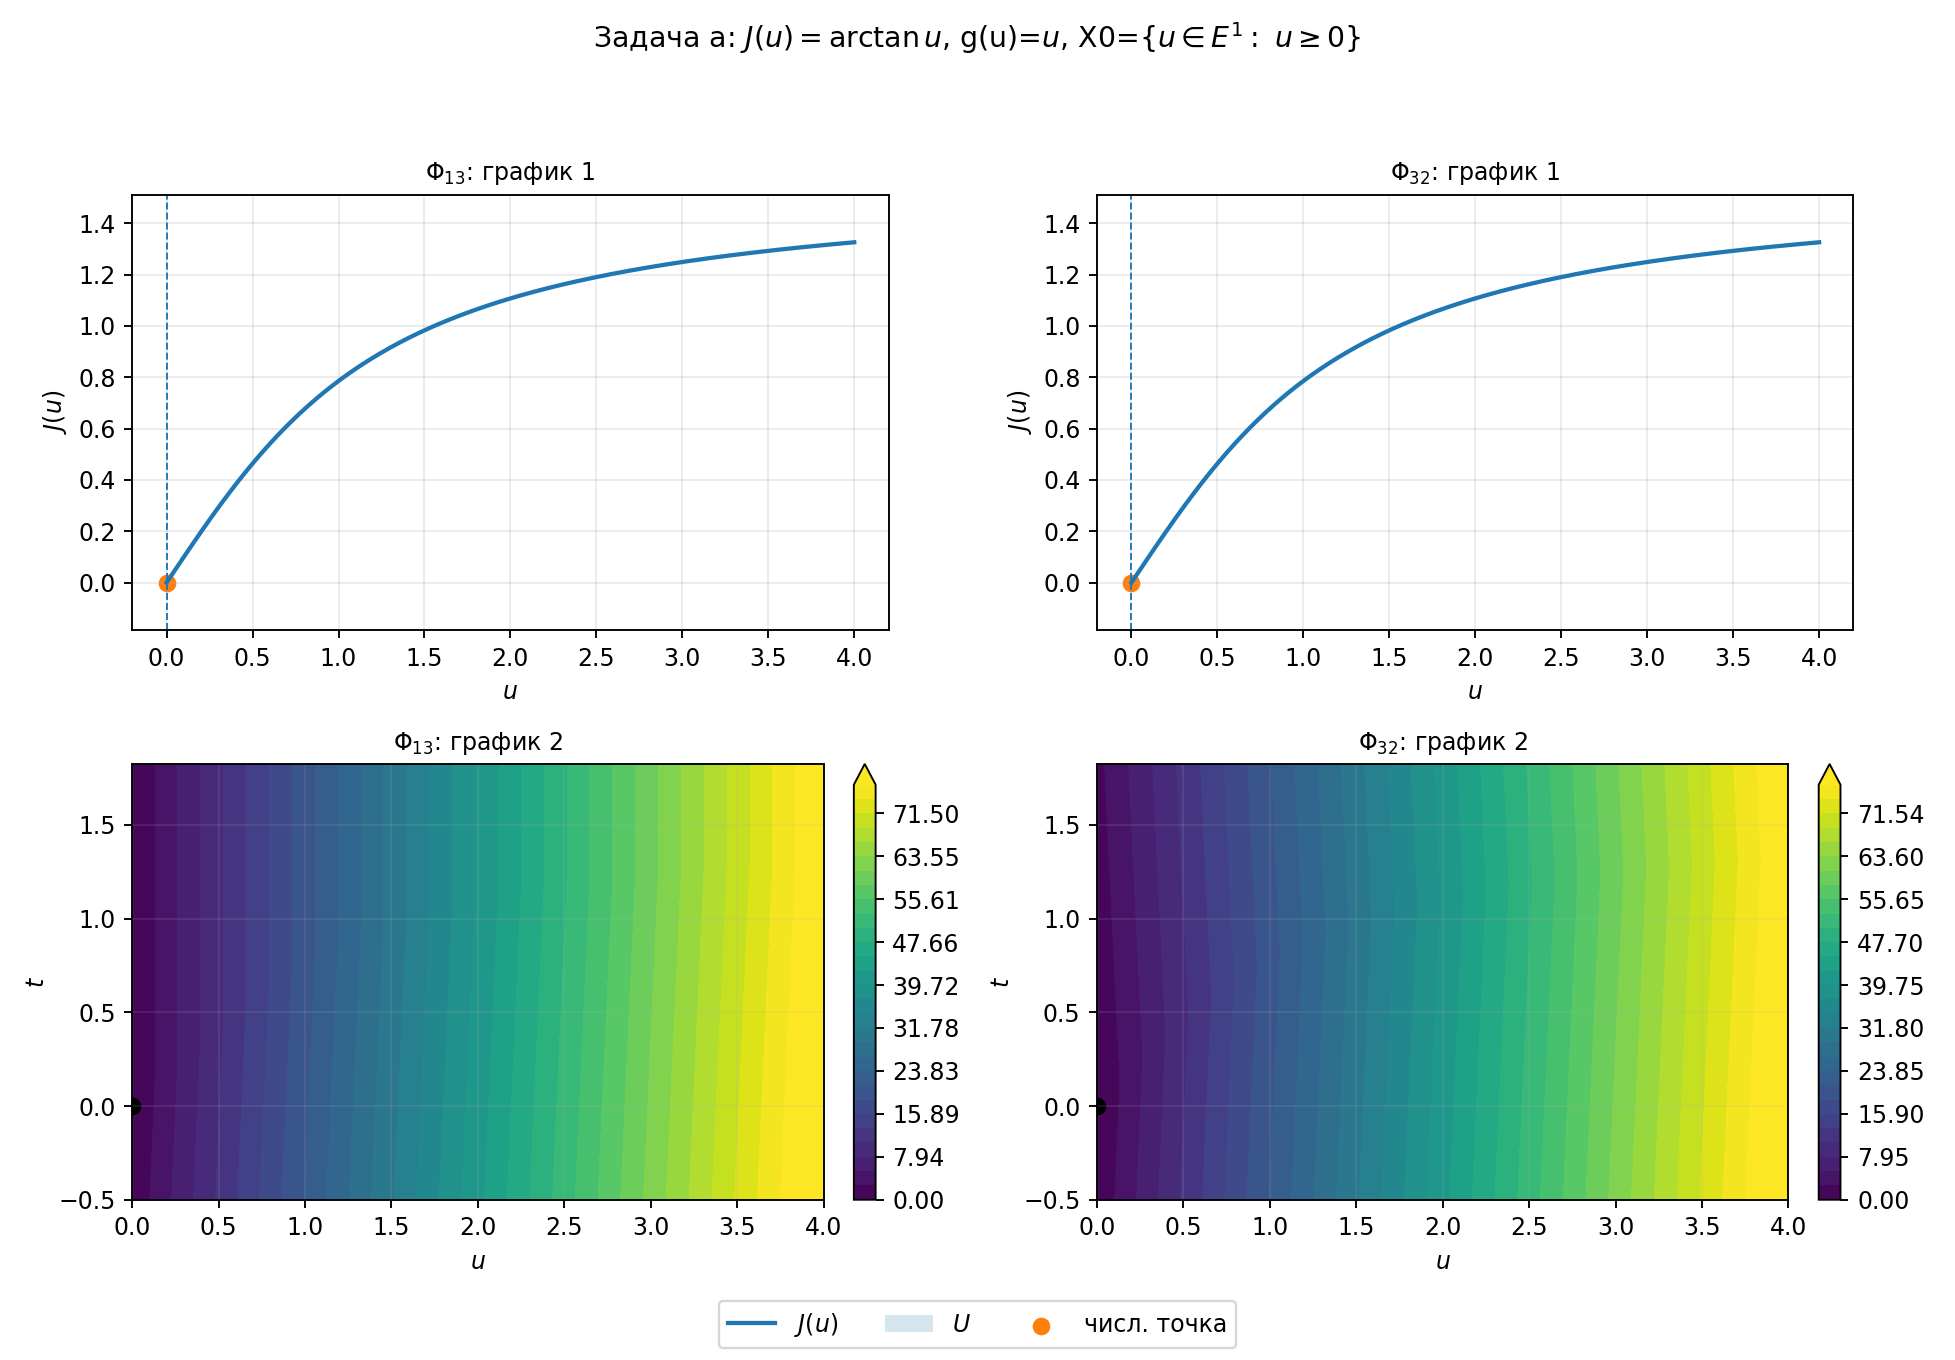
\includegraphics[width=0.96\textwidth]{graphs/a_g3_xge0_overview.png}
\caption{Задача а, вариант g3: $g(u)=u$, $X_0=\{u\in E^1:\ u\geq 0\}$. Верхний ряд: график 1 для $\Phi_{13}$ и $\Phi_{32}$; нижний ряд: график 2 для $\Phi_{13}$ и $\Phi_{32}$.}
\end{figure}

\begin{figure}[H]
\centering
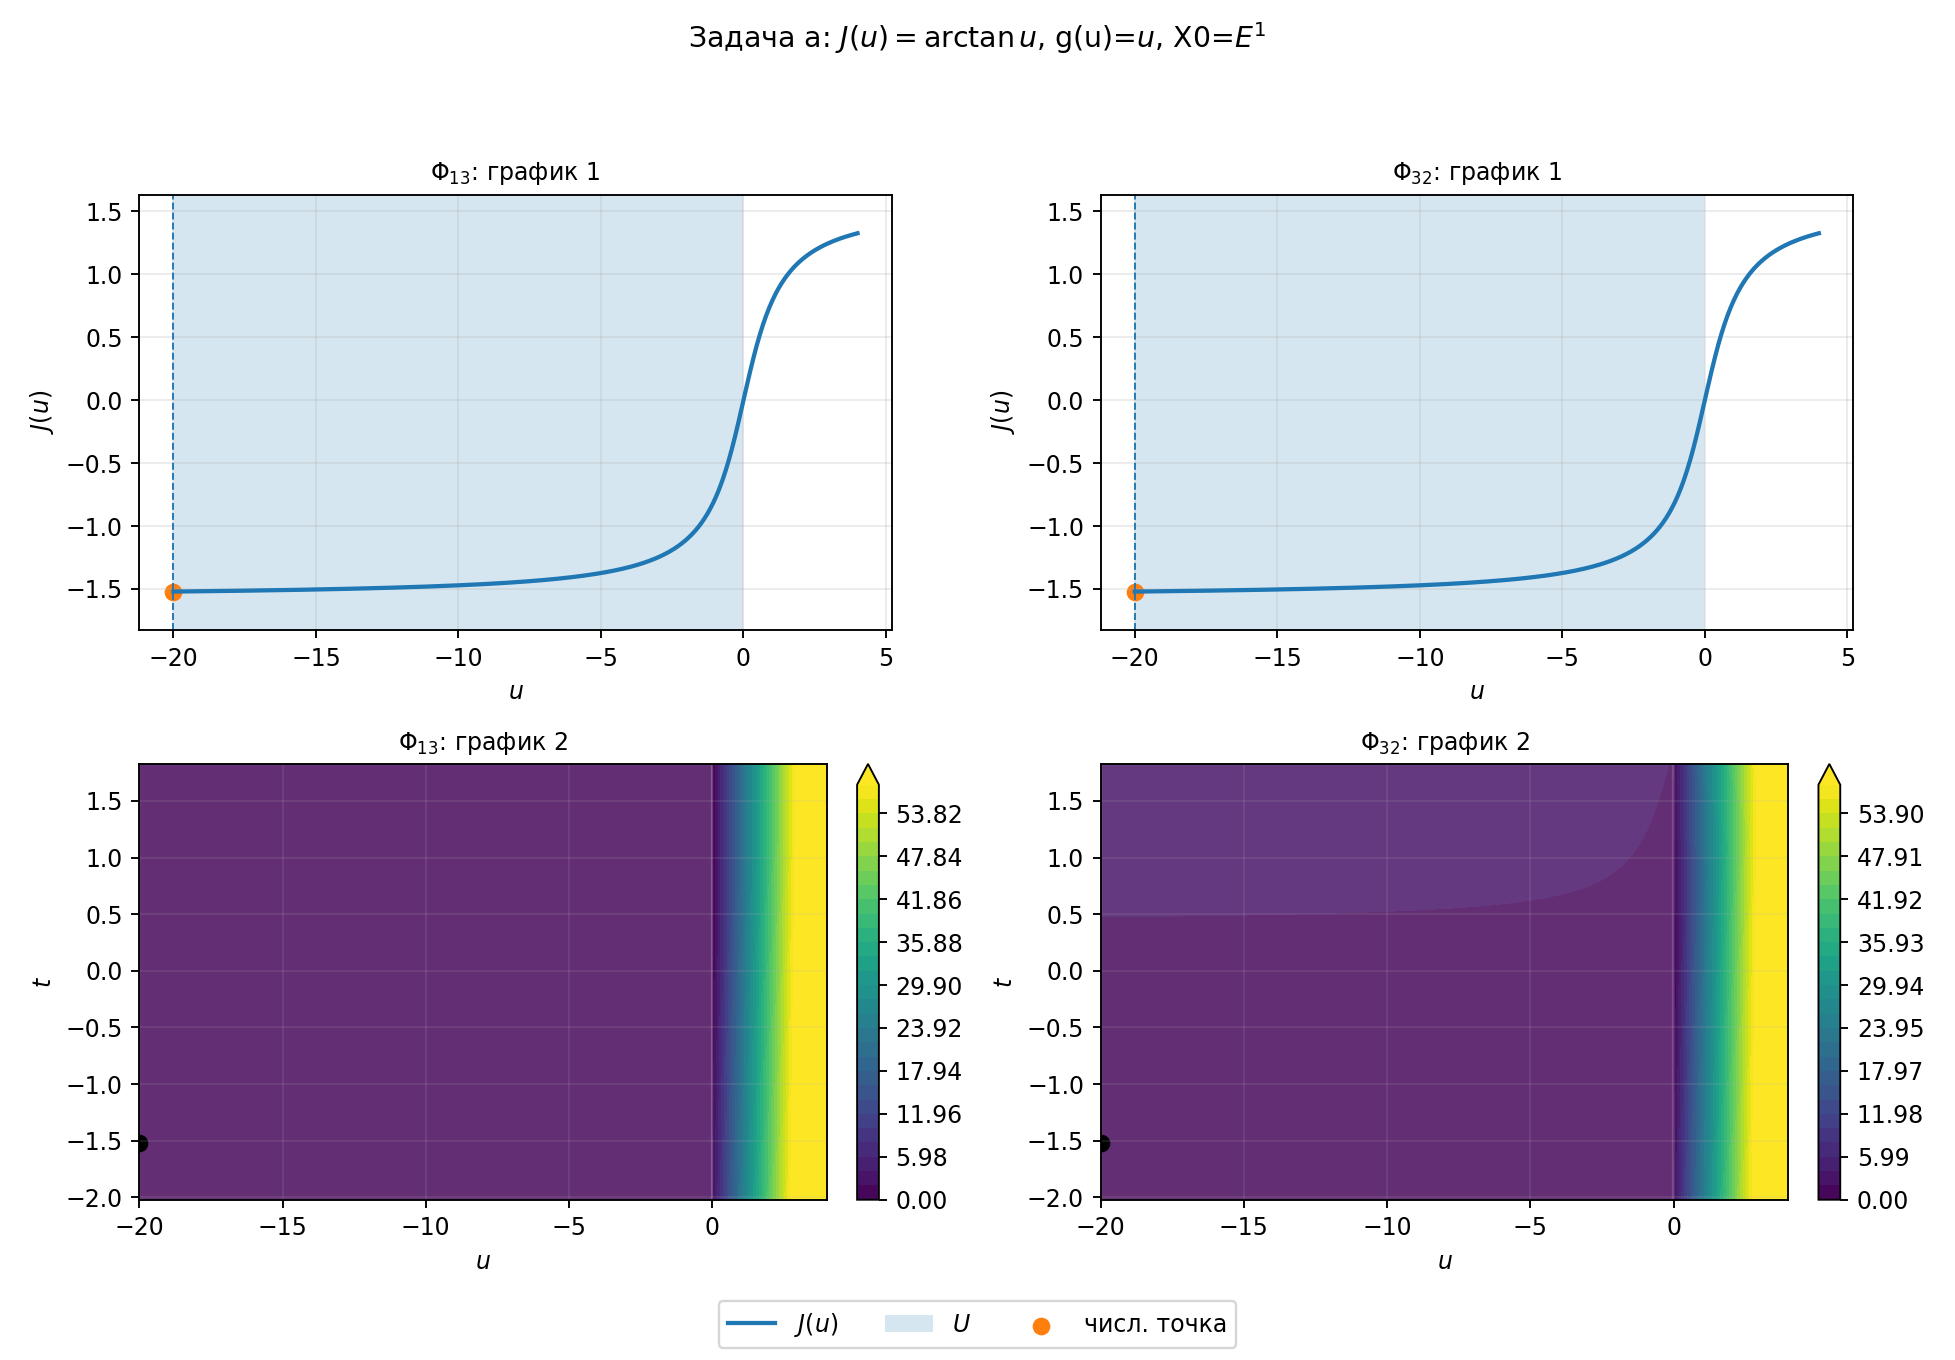
\includegraphics[width=0.96\textwidth]{graphs/a_g3_R_overview.png}
\caption{Задача а, вариант g3: $g(u)=u$, $X_0=E^1$. Верхний ряд: график 1 для $\Phi_{13}$ и $\Phi_{32}$; нижний ряд: график 2 для $\Phi_{13}$ и $\Phi_{32}$.}
\end{figure}

\begin{figure}[H]
\centering
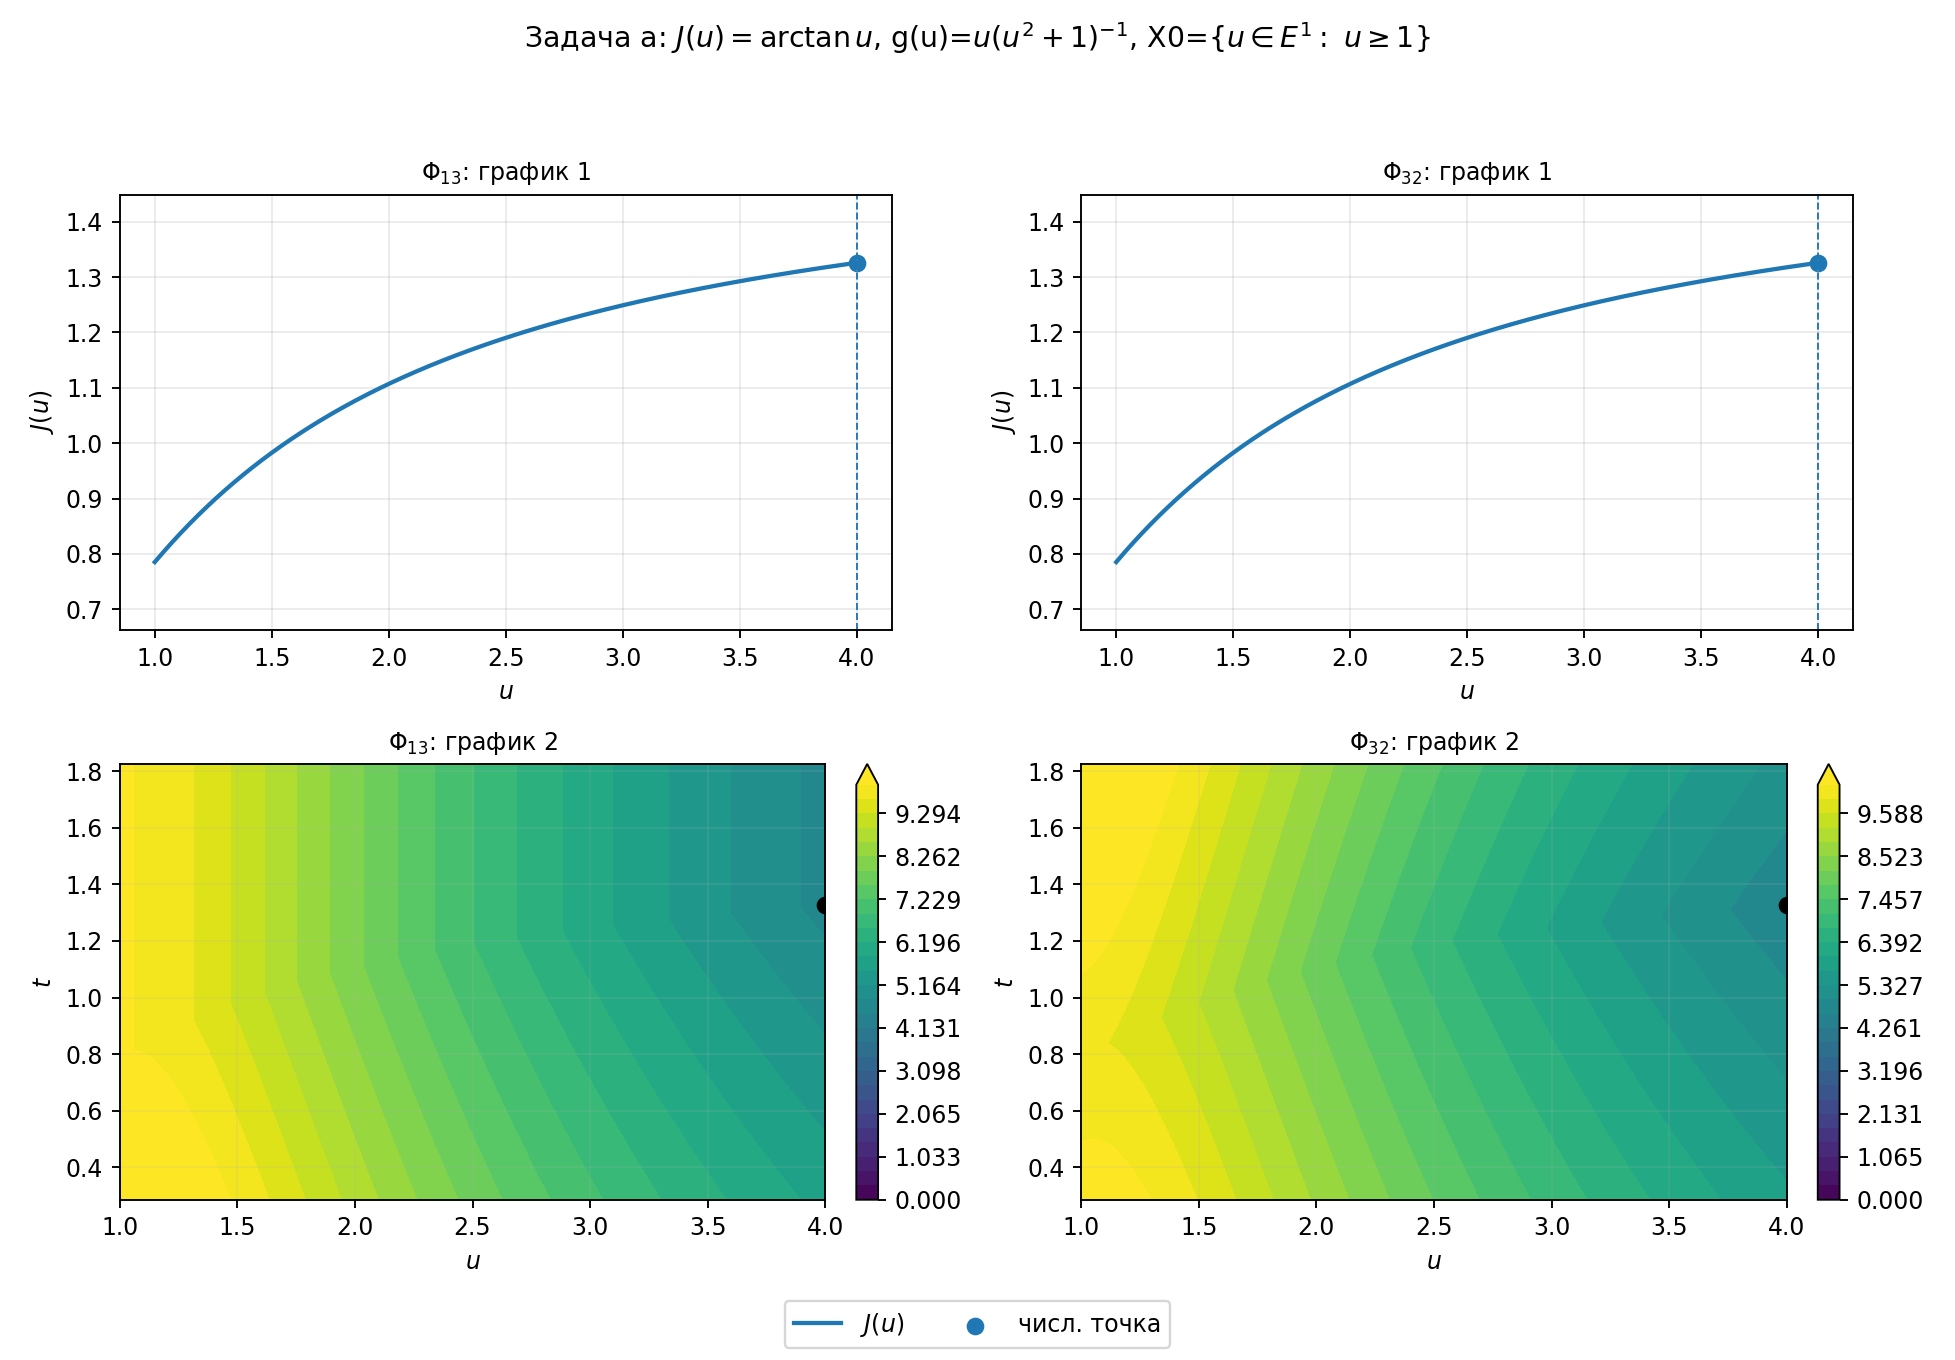
\includegraphics[width=0.96\textwidth]{graphs/a_g4_xge1_overview.png}
\caption{Задача а, вариант g4: $g(u)=u(u^2+1)^{-1}$, $X_0=\{u\in E^1:\ u\geq 1\}$. Верхний ряд: график 1 для $\Phi_{13}$ и $\Phi_{32}$; нижний ряд: график 2 для $\Phi_{13}$ и $\Phi_{32}$.}
\end{figure}

\begin{figure}[H]
\centering
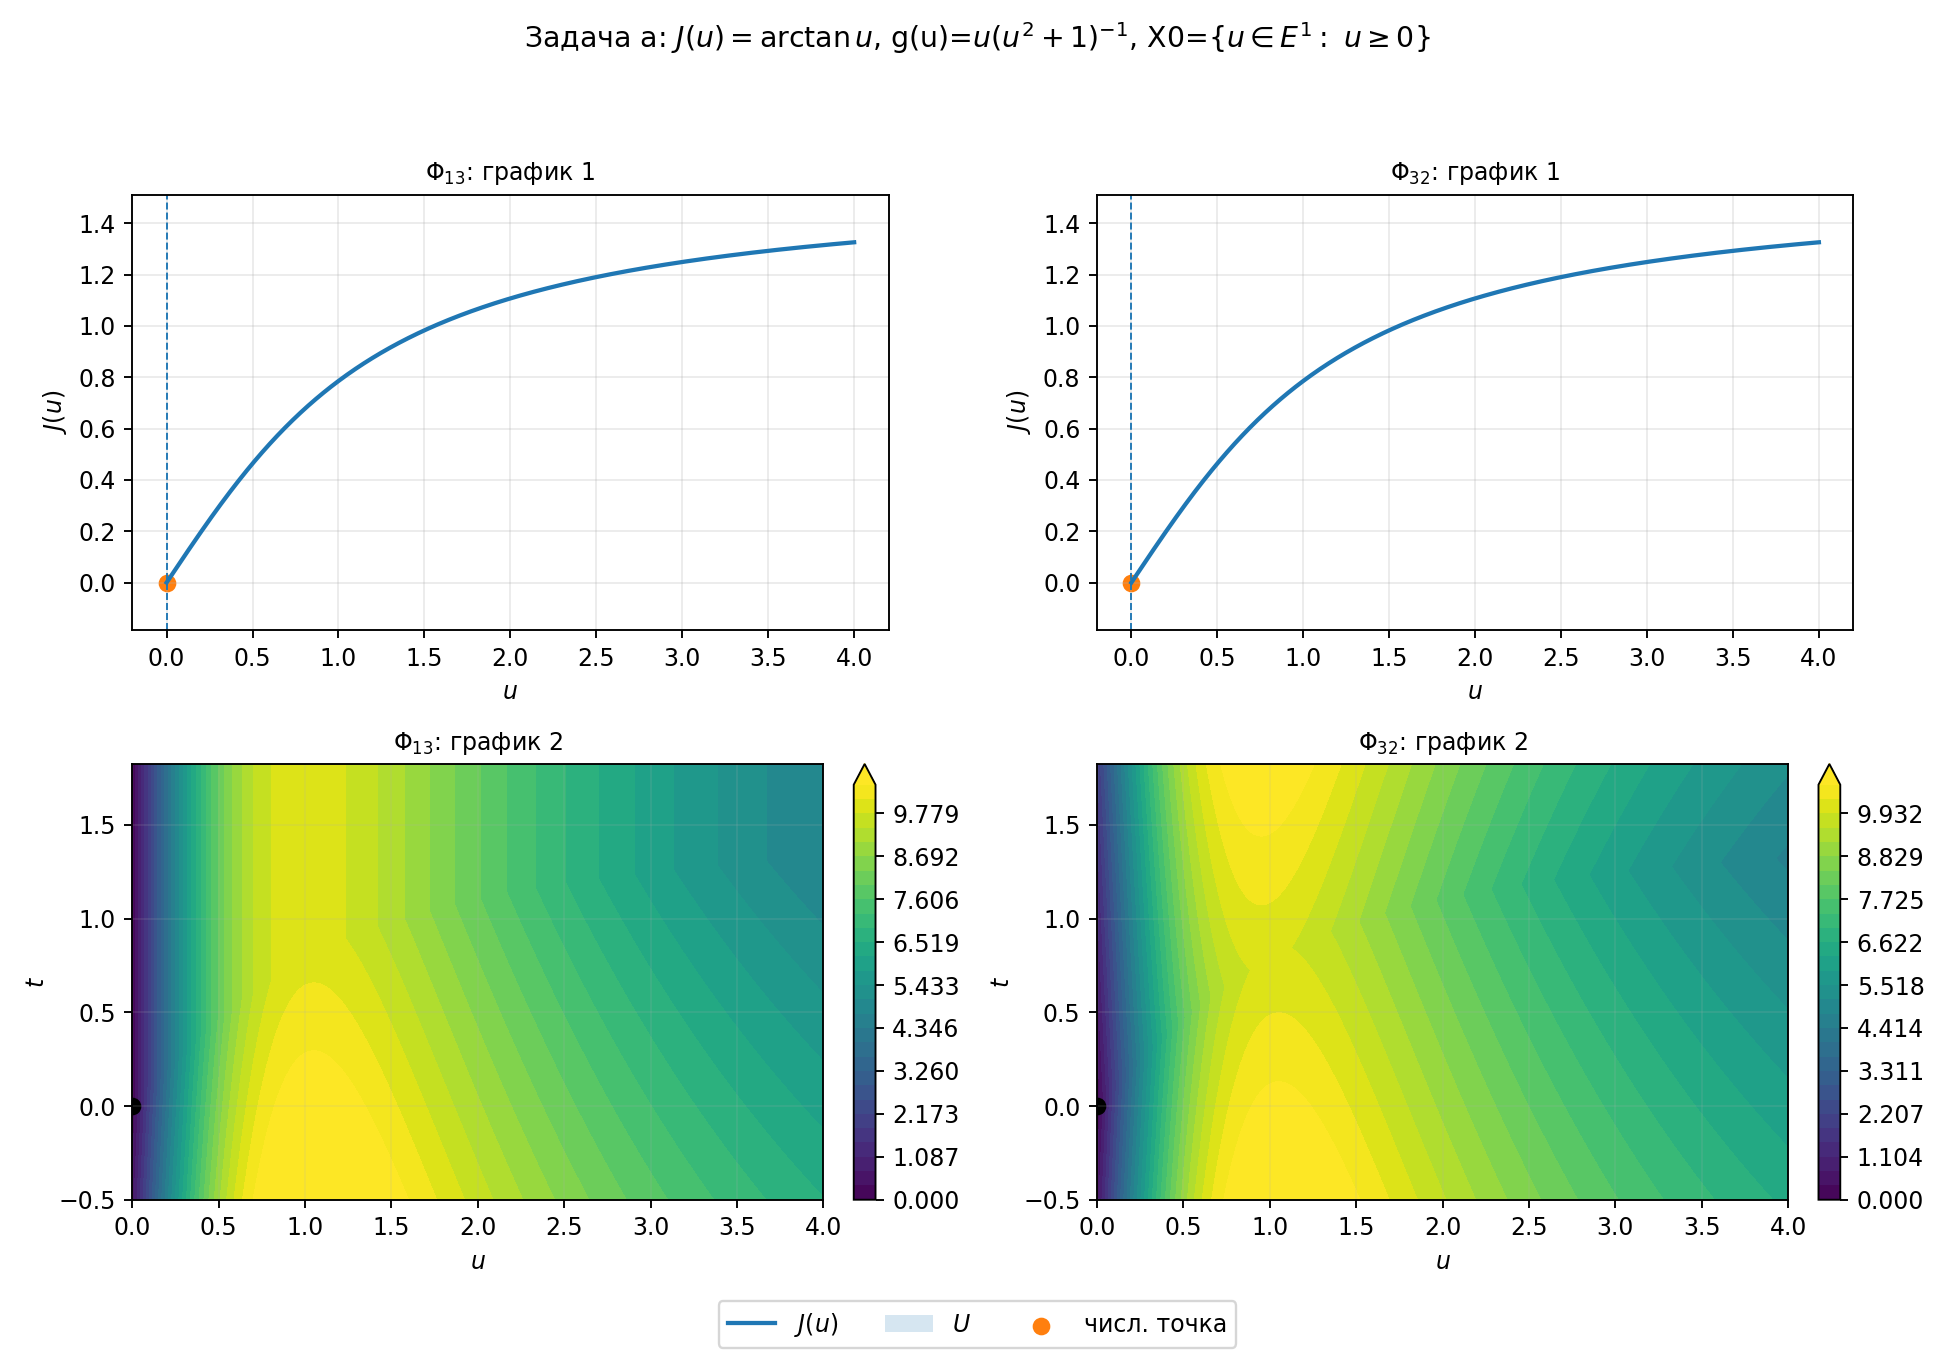
\includegraphics[width=0.96\textwidth]{graphs/a_g4_xge0_overview.png}
\caption{Задача а, вариант g4: $g(u)=u(u^2+1)^{-1}$, $X_0=\{u\in E^1:\ u\geq 0\}$. Верхний ряд: график 1 для $\Phi_{13}$ и $\Phi_{32}$; нижний ряд: график 2 для $\Phi_{13}$ и $\Phi_{32}$.}
\end{figure}

\begin{figure}[H]
\centering
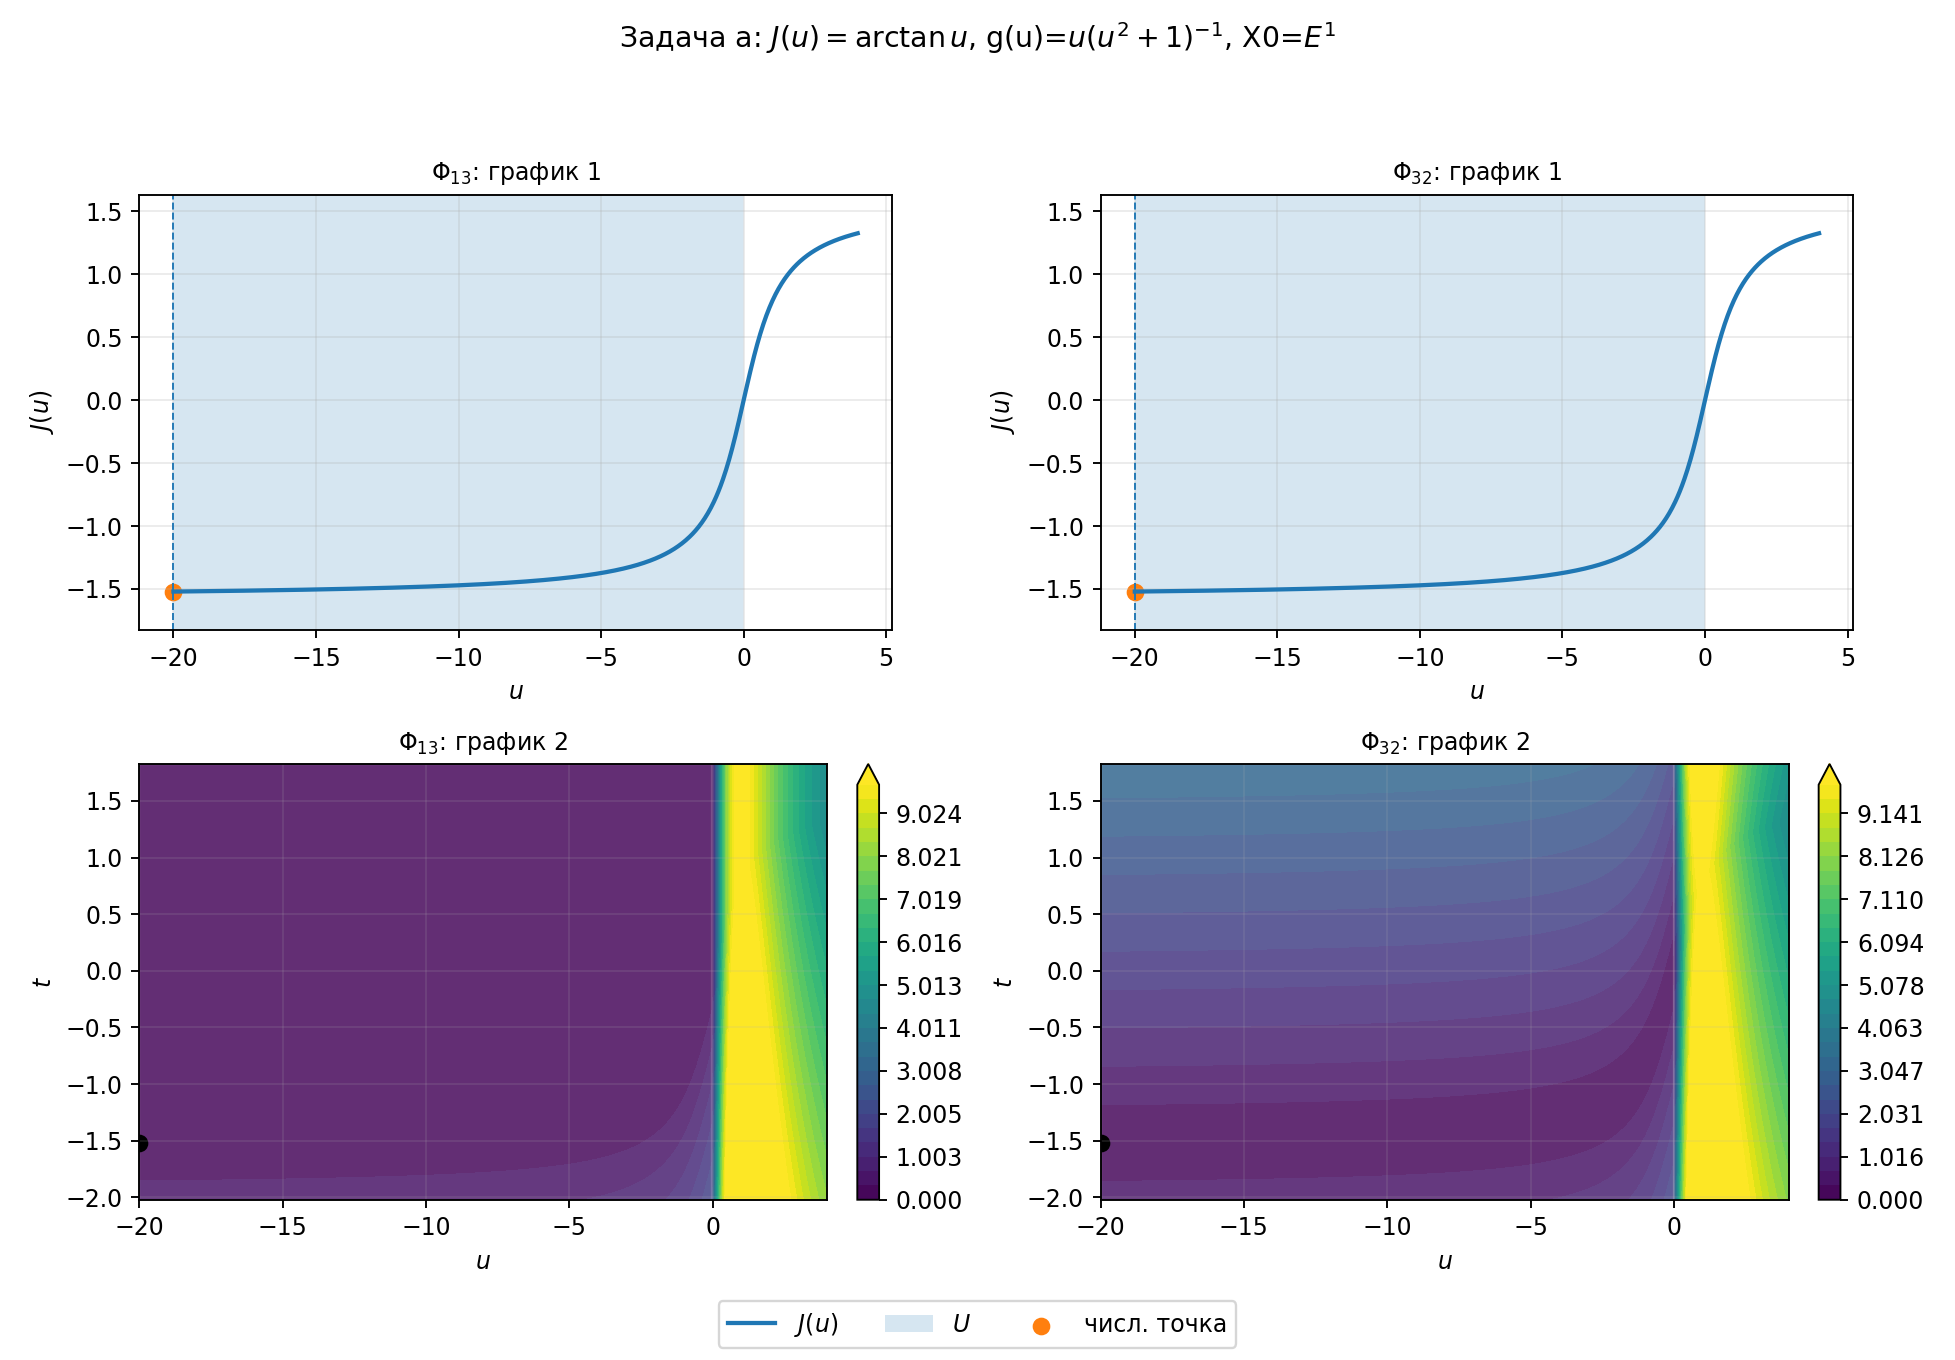
\includegraphics[width=0.96\textwidth]{graphs/a_g4_R_overview.png}
\caption{Задача а, вариант g4: $g(u)=u(u^2+1)^{-1}$, $X_0=E^1$. Верхний ряд: график 1 для $\Phi_{13}$ и $\Phi_{32}$; нижний ряд: график 2 для $\Phi_{13}$ и $\Phi_{32}$.}
\end{figure}

\begin{figure}[H]
\centering
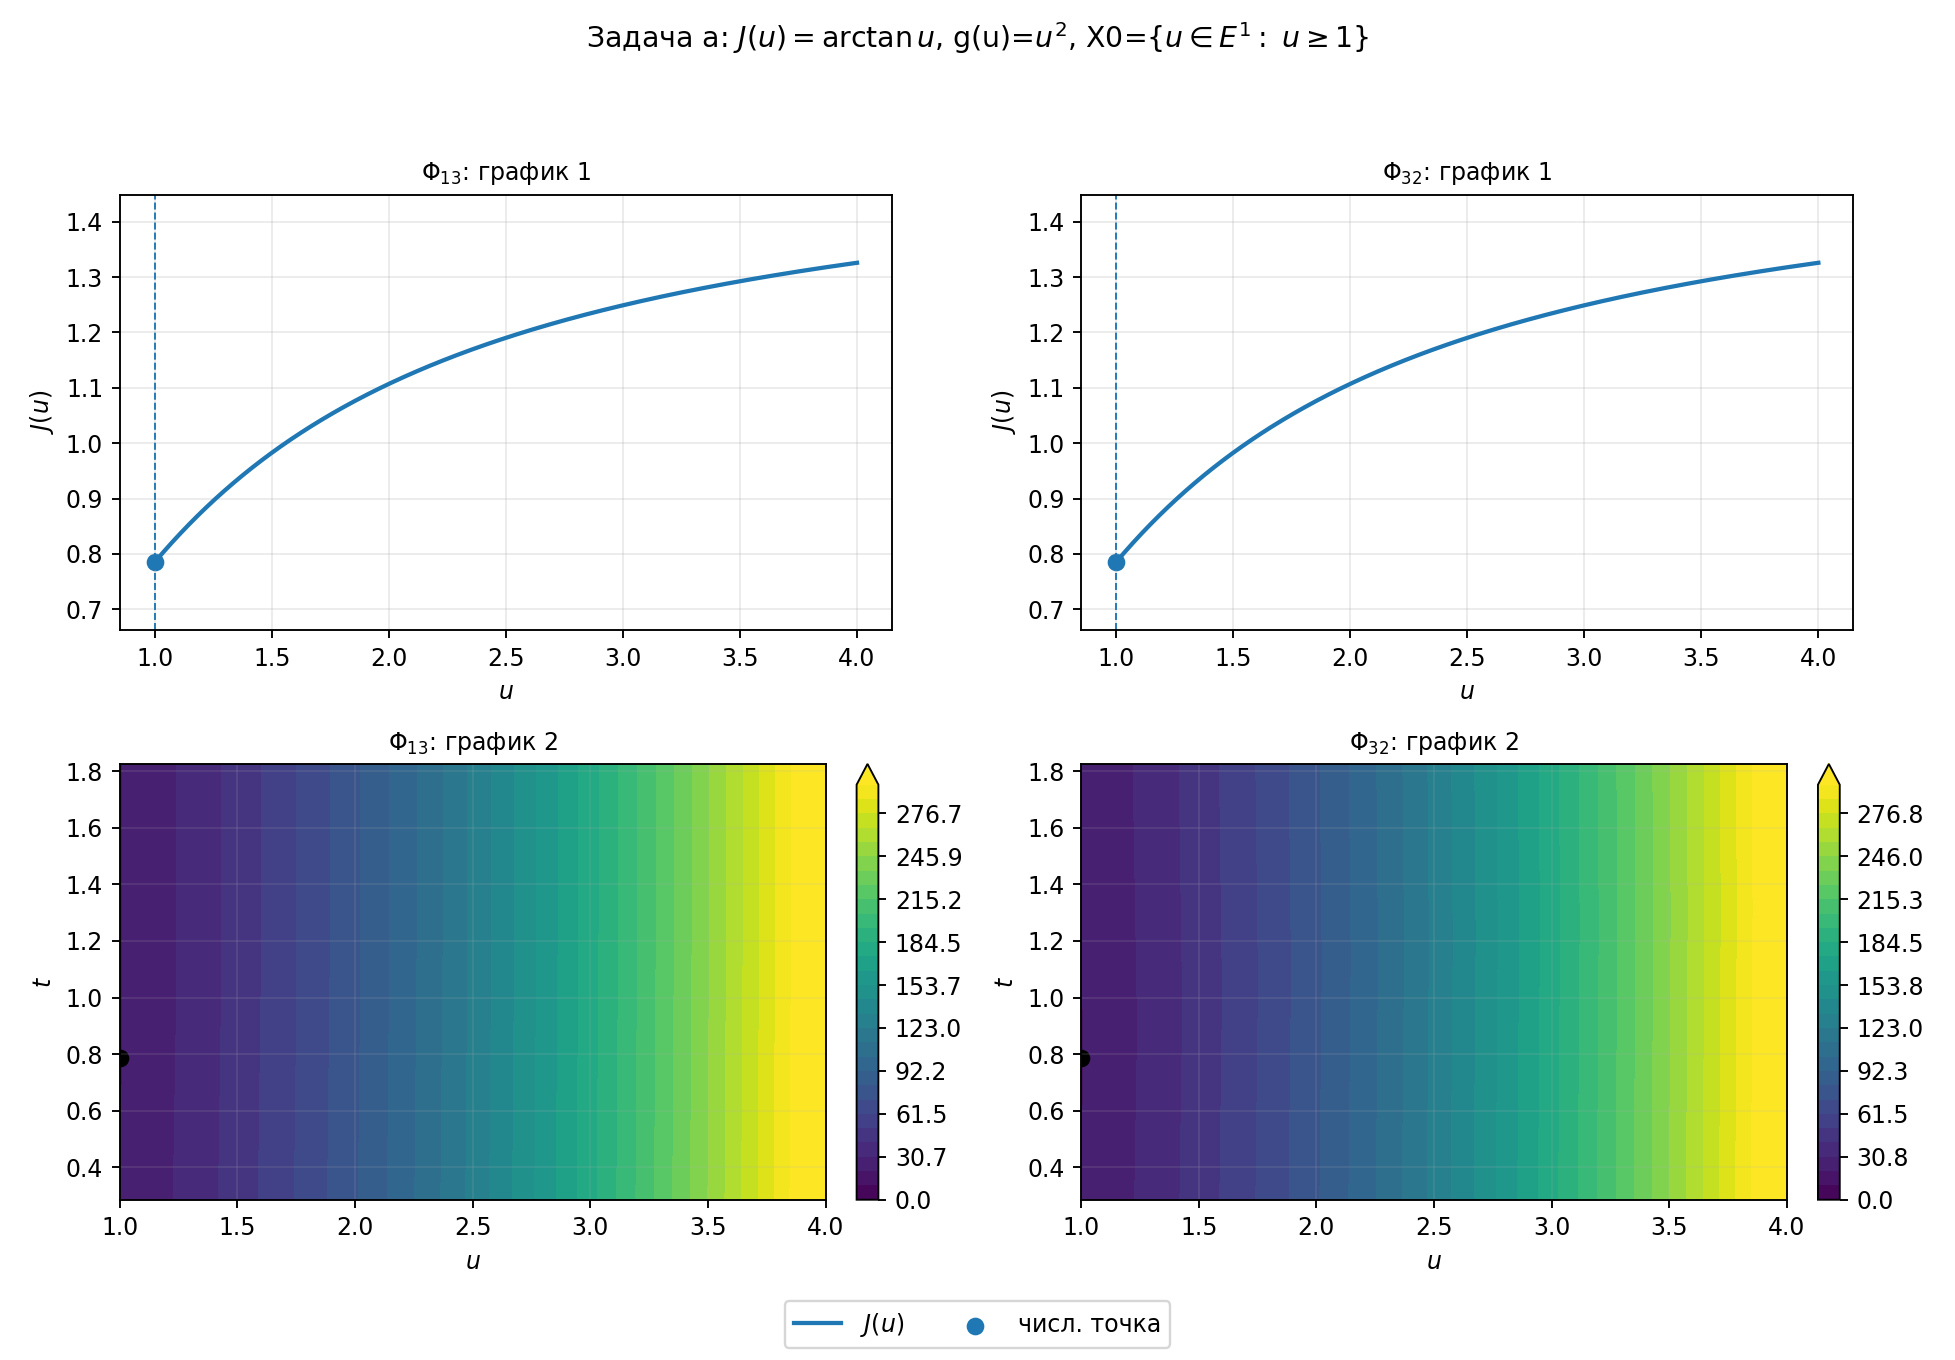
\includegraphics[width=0.96\textwidth]{graphs/a_g5_xge1_overview.png}
\caption{Задача а, вариант g5: $g(u)=u^2$, $X_0=\{u\in E^1:\ u\geq 1\}$. Верхний ряд: график 1 для $\Phi_{13}$ и $\Phi_{32}$; нижний ряд: график 2 для $\Phi_{13}$ и $\Phi_{32}$.}
\end{figure}

\begin{figure}[H]
\centering
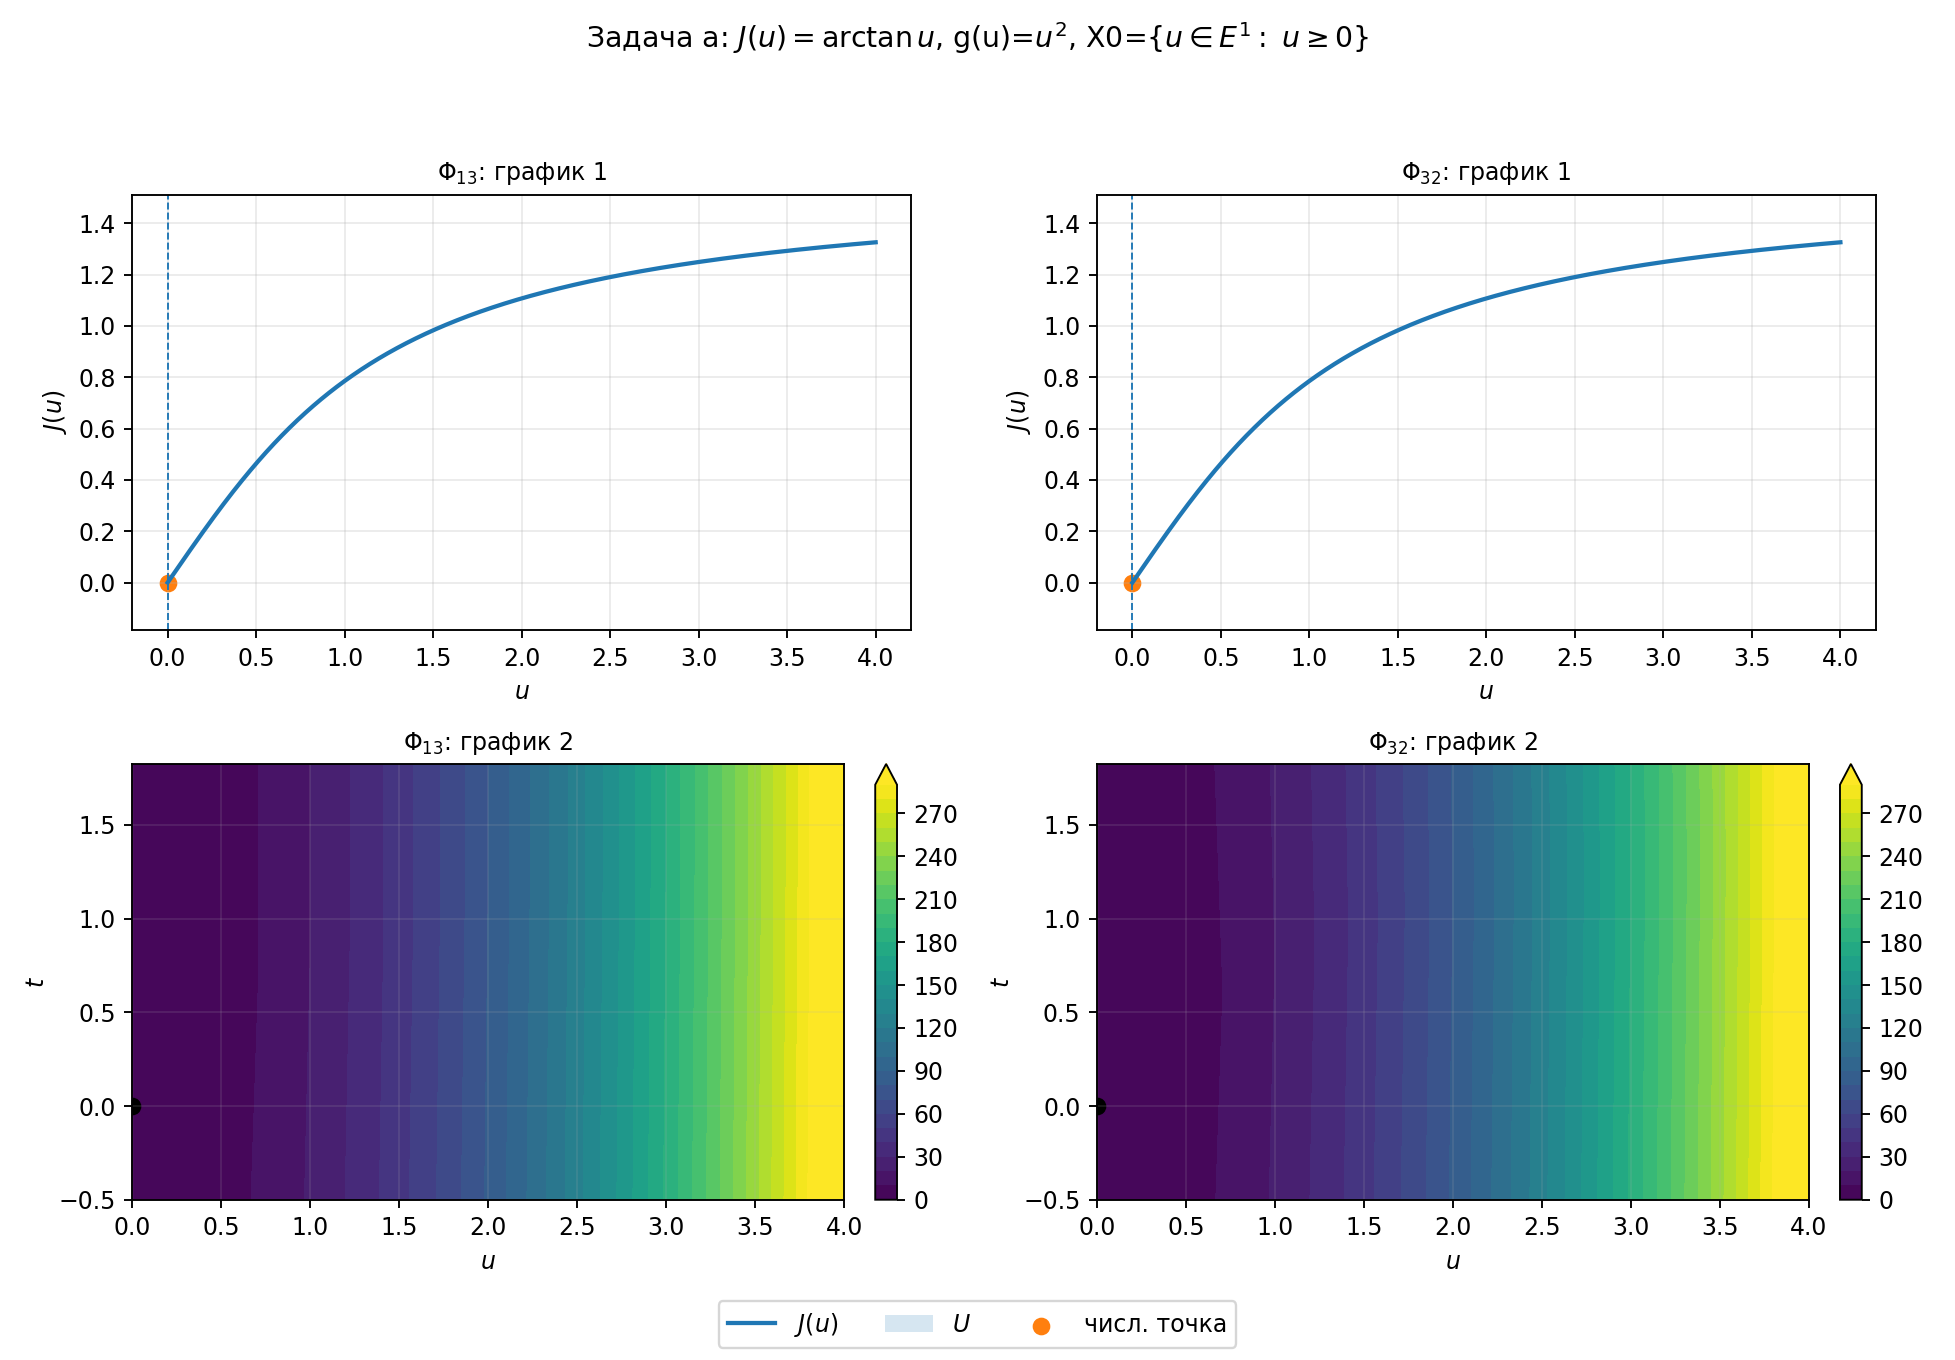
\includegraphics[width=0.96\textwidth]{graphs/a_g5_xge0_overview.png}
\caption{Задача а, вариант g5: $g(u)=u^2$, $X_0=\{u\in E^1:\ u\geq 0\}$. Верхний ряд: график 1 для $\Phi_{13}$ и $\Phi_{32}$; нижний ряд: график 2 для $\Phi_{13}$ и $\Phi_{32}$.}
\end{figure}

\begin{figure}[H]
\centering
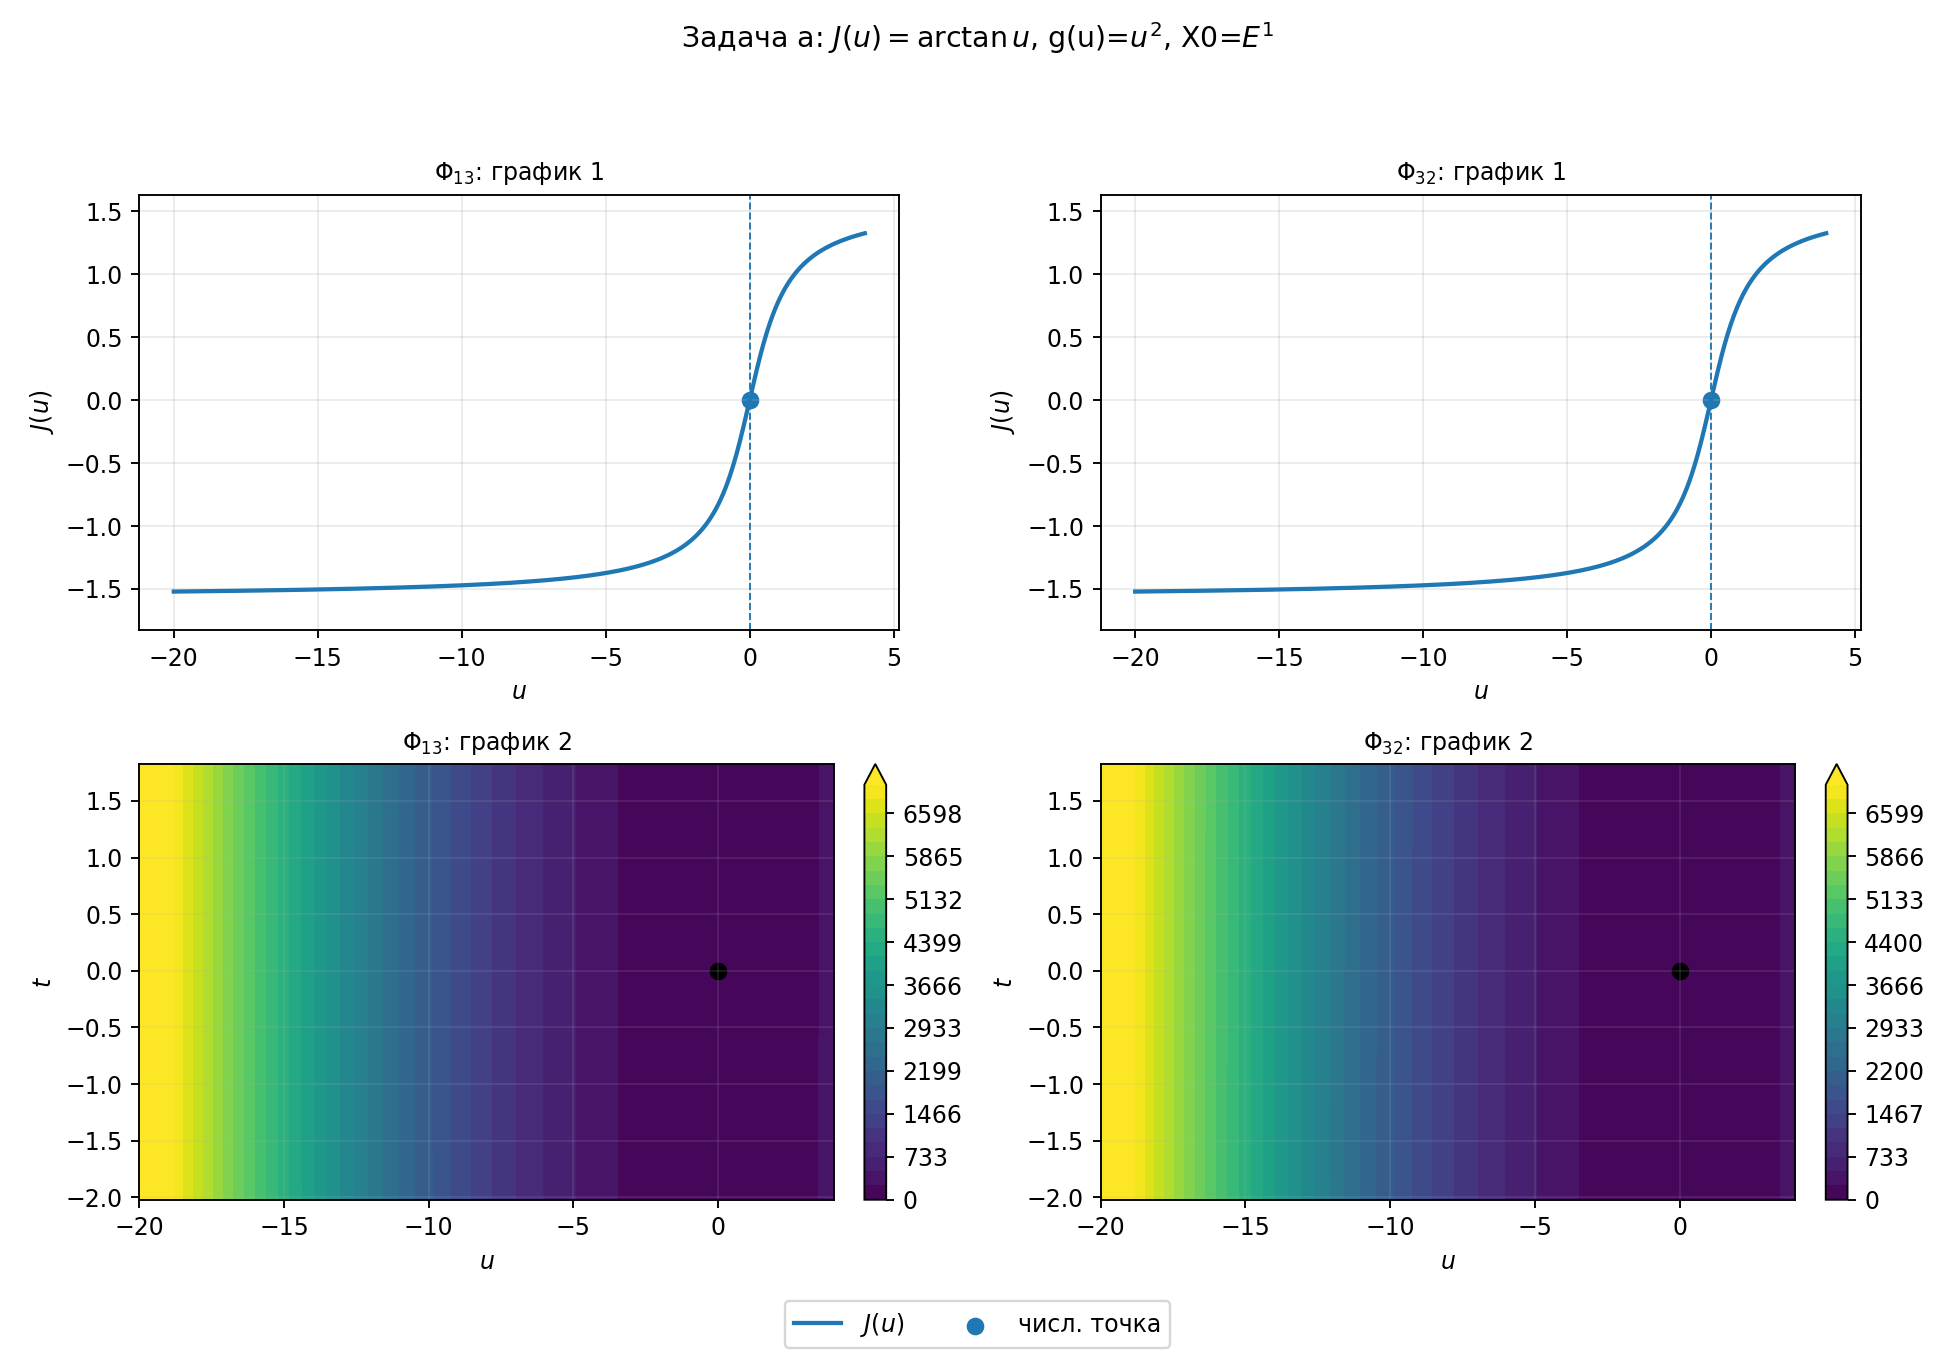
\includegraphics[width=0.96\textwidth]{graphs/a_g5_R_overview.png}
\caption{Задача а, вариант g5: $g(u)=u^2$, $X_0=E^1$. Верхний ряд: график 1 для $\Phi_{13}$ и $\Phi_{32}$; нижний ряд: график 2 для $\Phi_{13}$ и $\Phi_{32}$.}
\end{figure}

\begin{figure}[H]
\centering
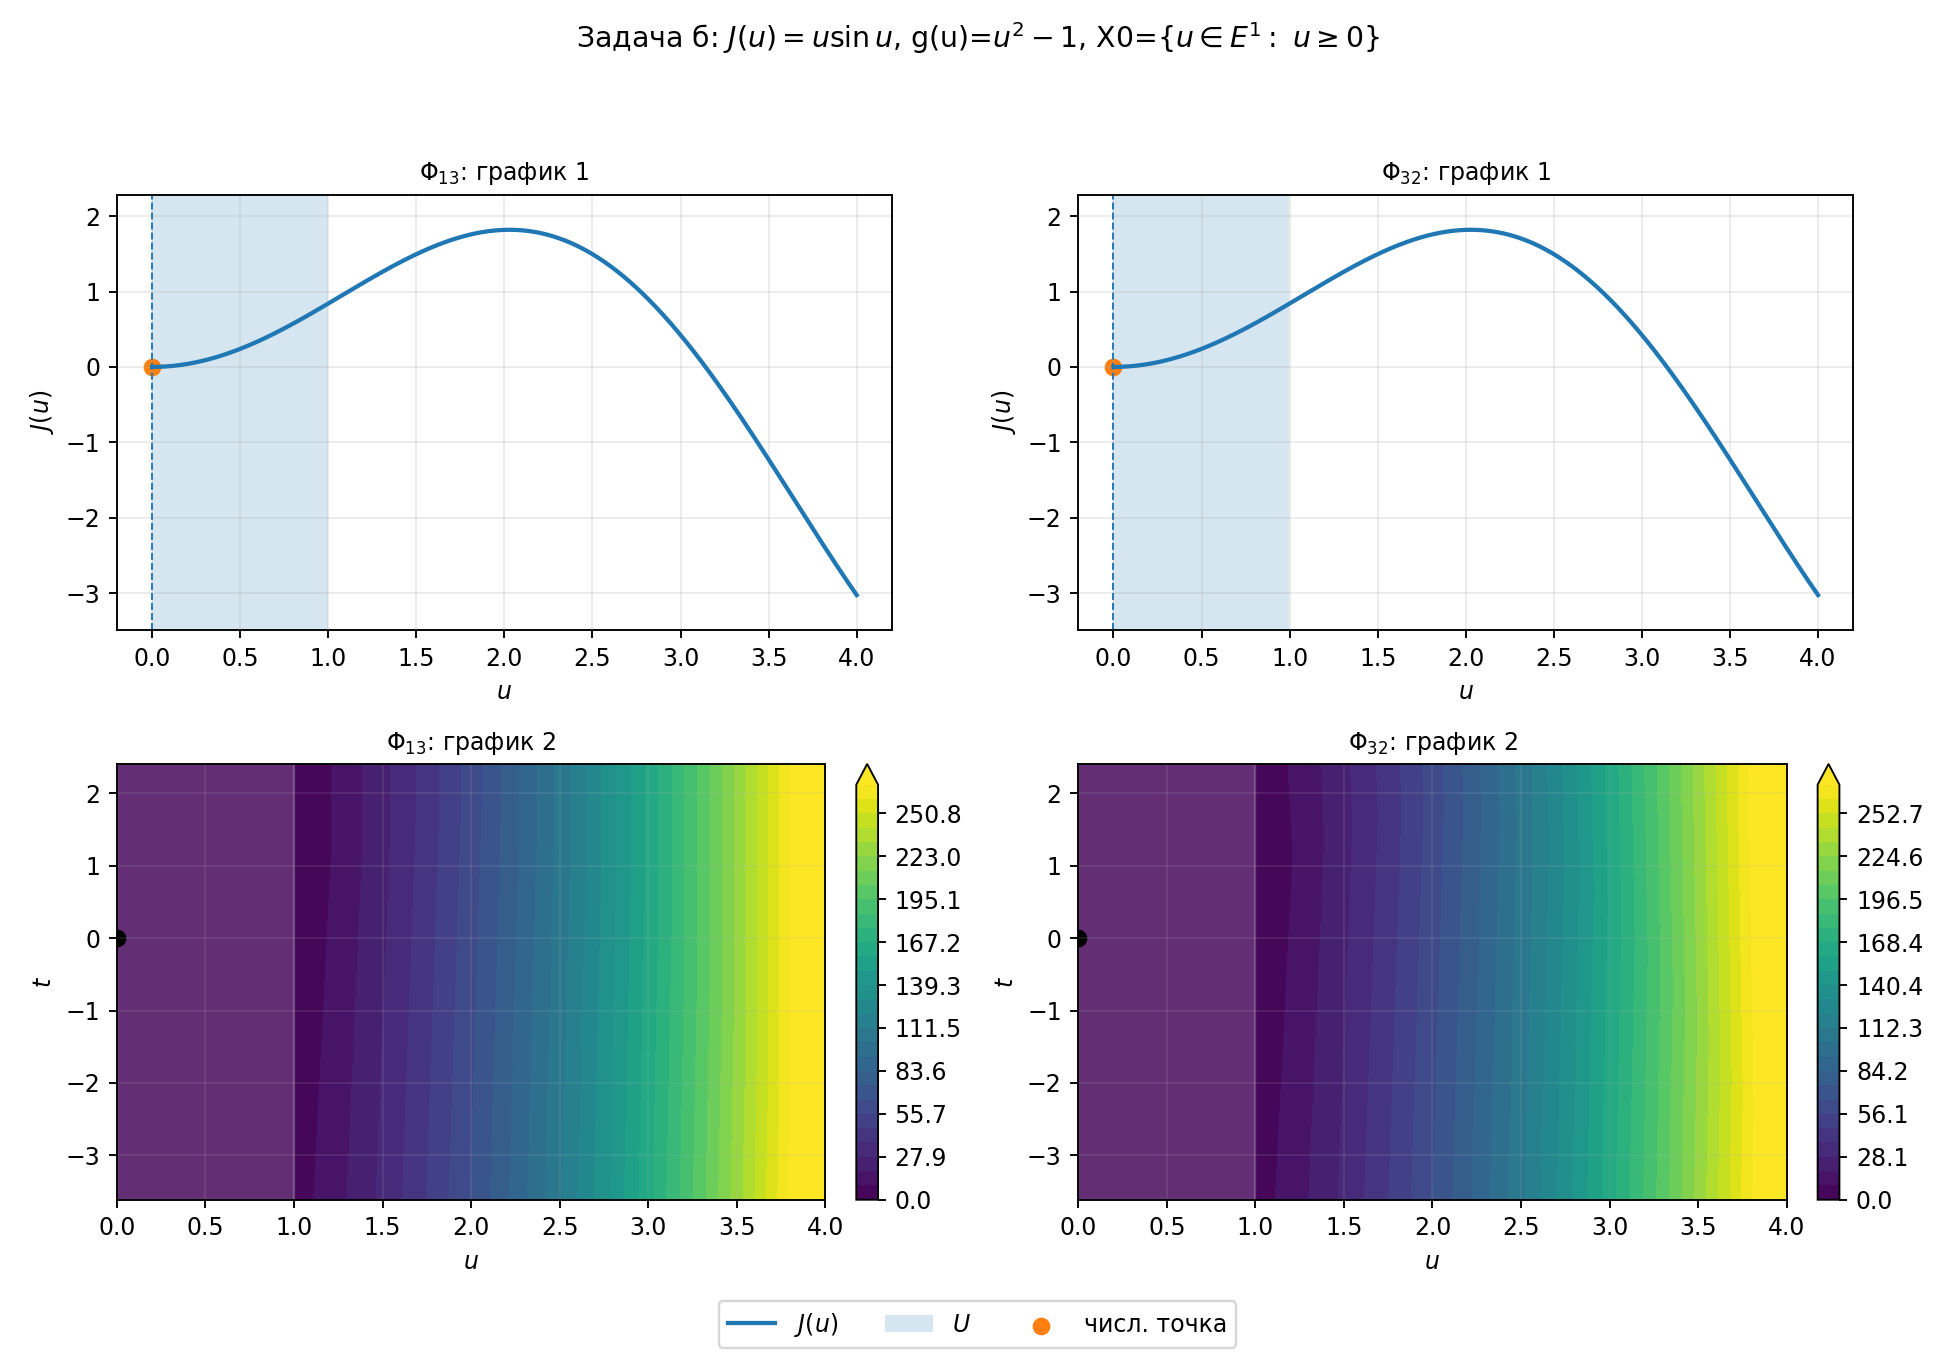
\includegraphics[width=0.96\textwidth]{graphs/b_g1_xge0_overview.png}
\caption{Задача б, вариант g1: $g(u)=u^2-1$, $X_0=\{u\in E^1:\ u\geq 0\}$. Верхний ряд: график 1 для $\Phi_{13}$ и $\Phi_{32}$; нижний ряд: график 2 для $\Phi_{13}$ и $\Phi_{32}$.}
\end{figure}

\begin{figure}[H]
\centering
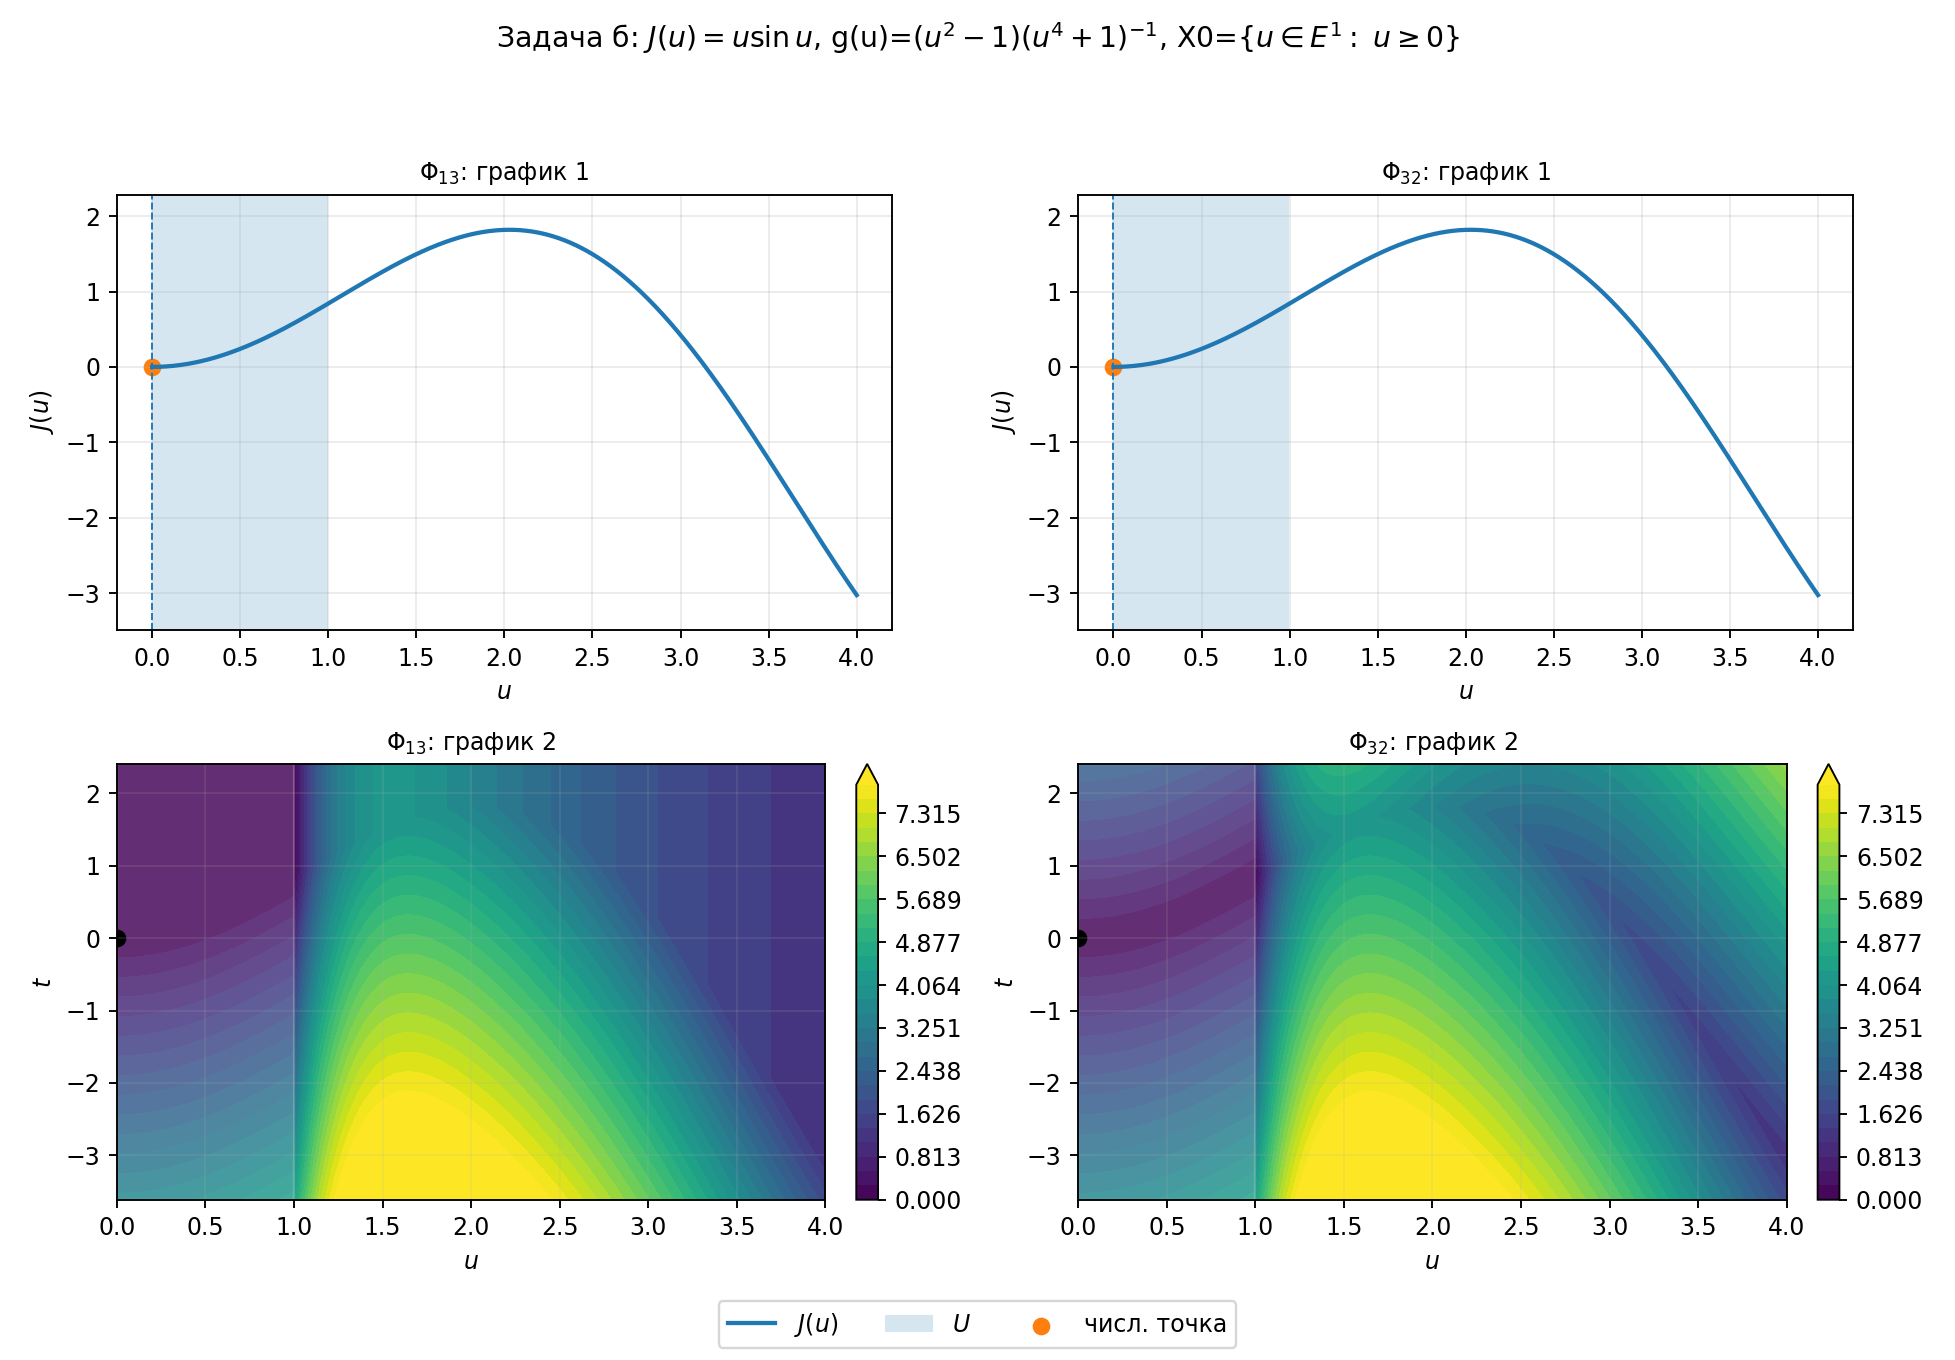
\includegraphics[width=0.96\textwidth]{graphs/b_g2_xge0_overview.png}
\caption{Задача б, вариант g2: $g(u)=(u^2-1)(u^4+1)^{-1}$, $X_0=\{u\in E^1:\ u\geq 0\}$. Верхний ряд: график 1 для $\Phi_{13}$ и $\Phi_{32}$; нижний ряд: график 2 для $\Phi_{13}$ и $\Phi_{32}$.}
\end{figure}

\begin{figure}[H]
\centering
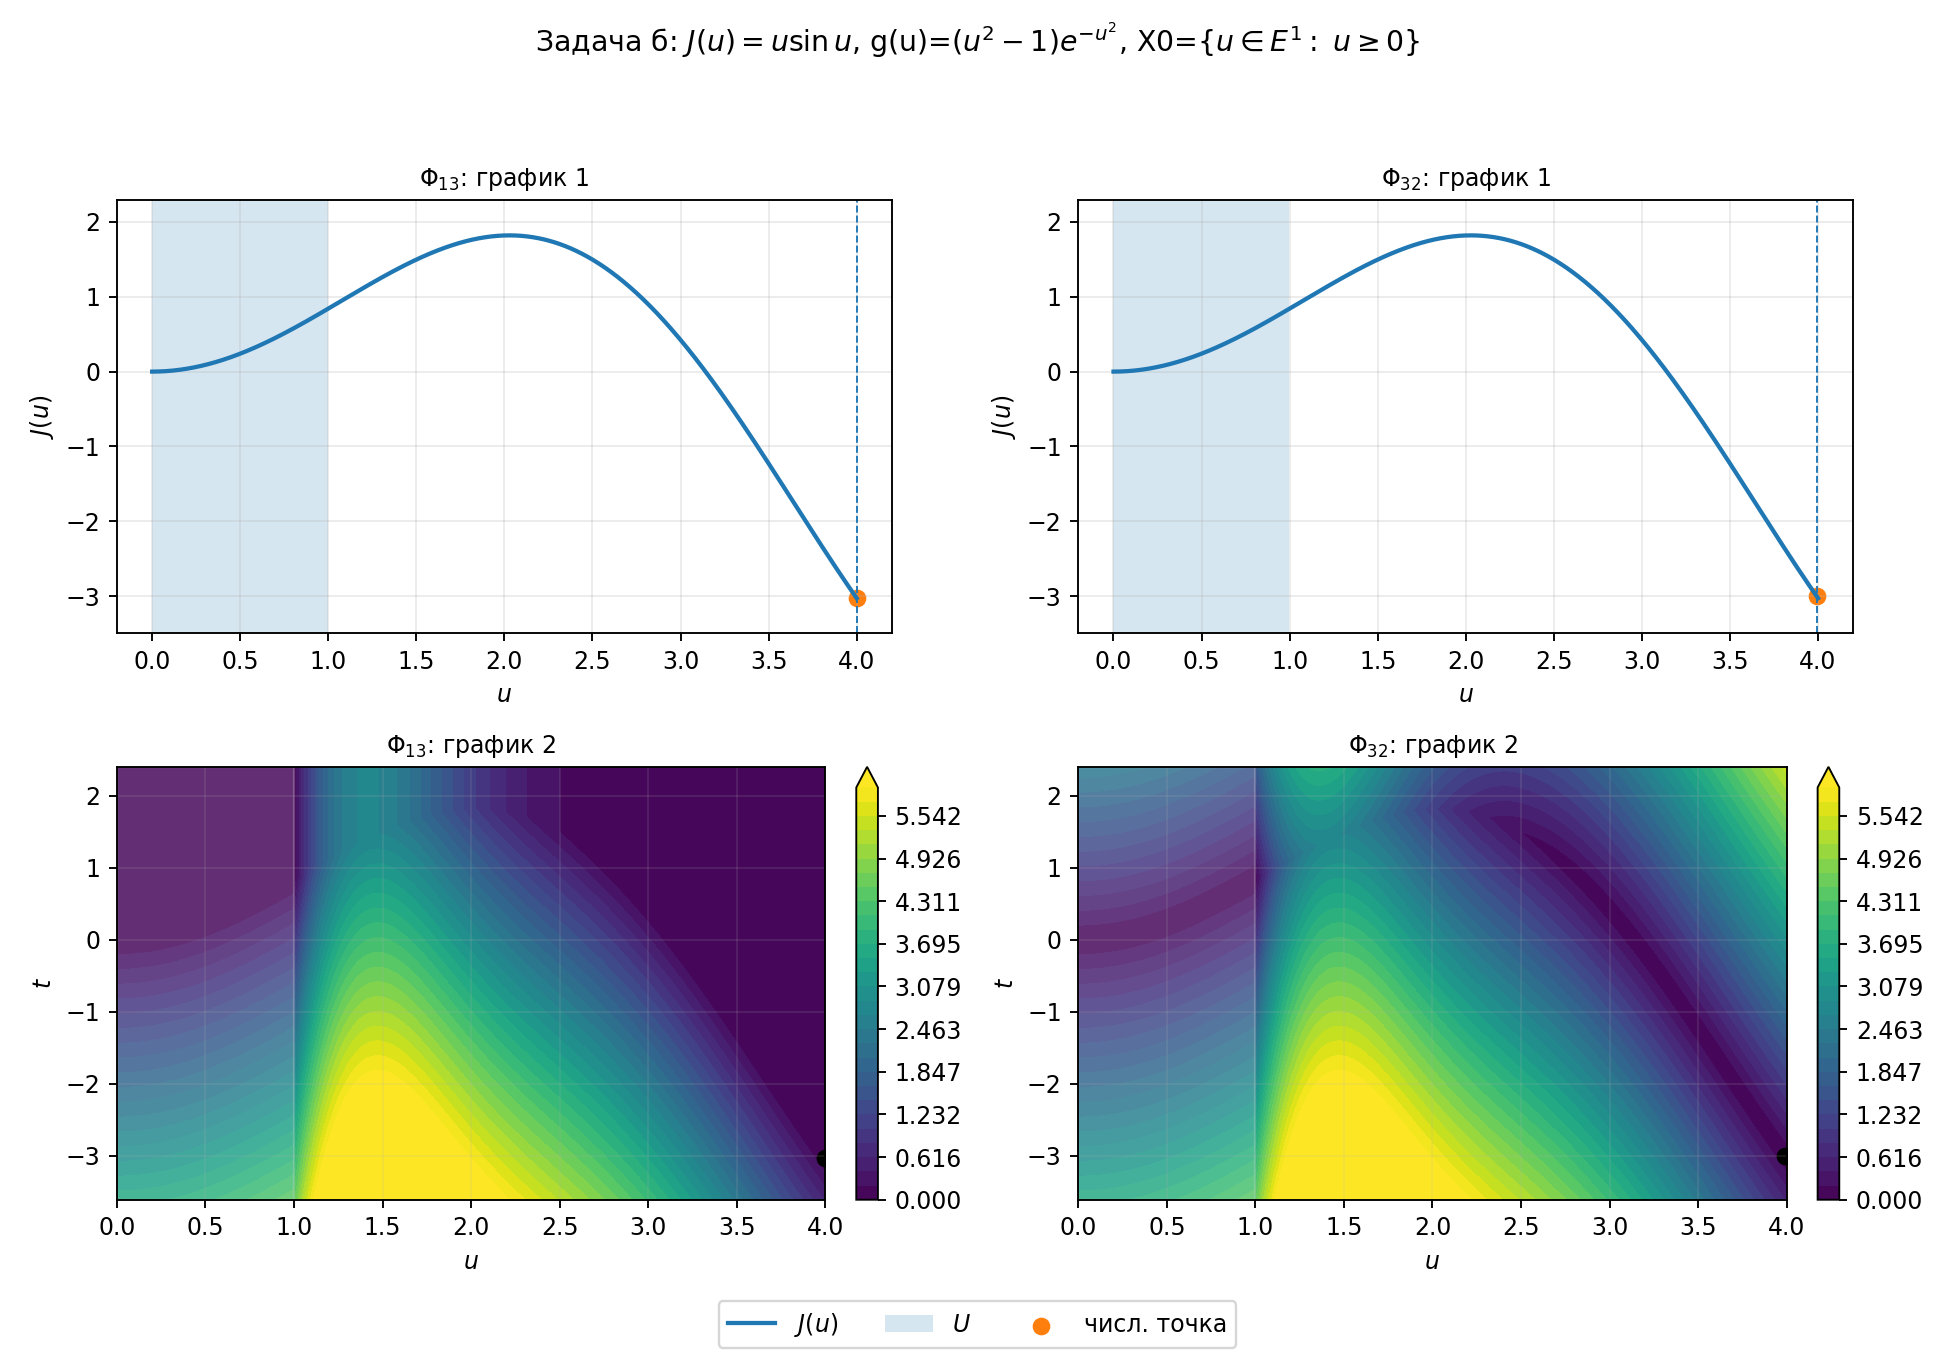
\includegraphics[width=0.96\textwidth]{graphs/b_g3_xge0_overview.png}
\caption{Задача б, вариант g3: $g(u)=(u^2-1)e^{-u^2}$, $X_0=\{u\in E^1:\ u\geq 0\}$. Верхний ряд: график 1 для $\Phi_{13}$ и $\Phi_{32}$; нижний ряд: график 2 для $\Phi_{13}$ и $\Phi_{32}$.}
\end{figure}

\begin{figure}[H]
\centering
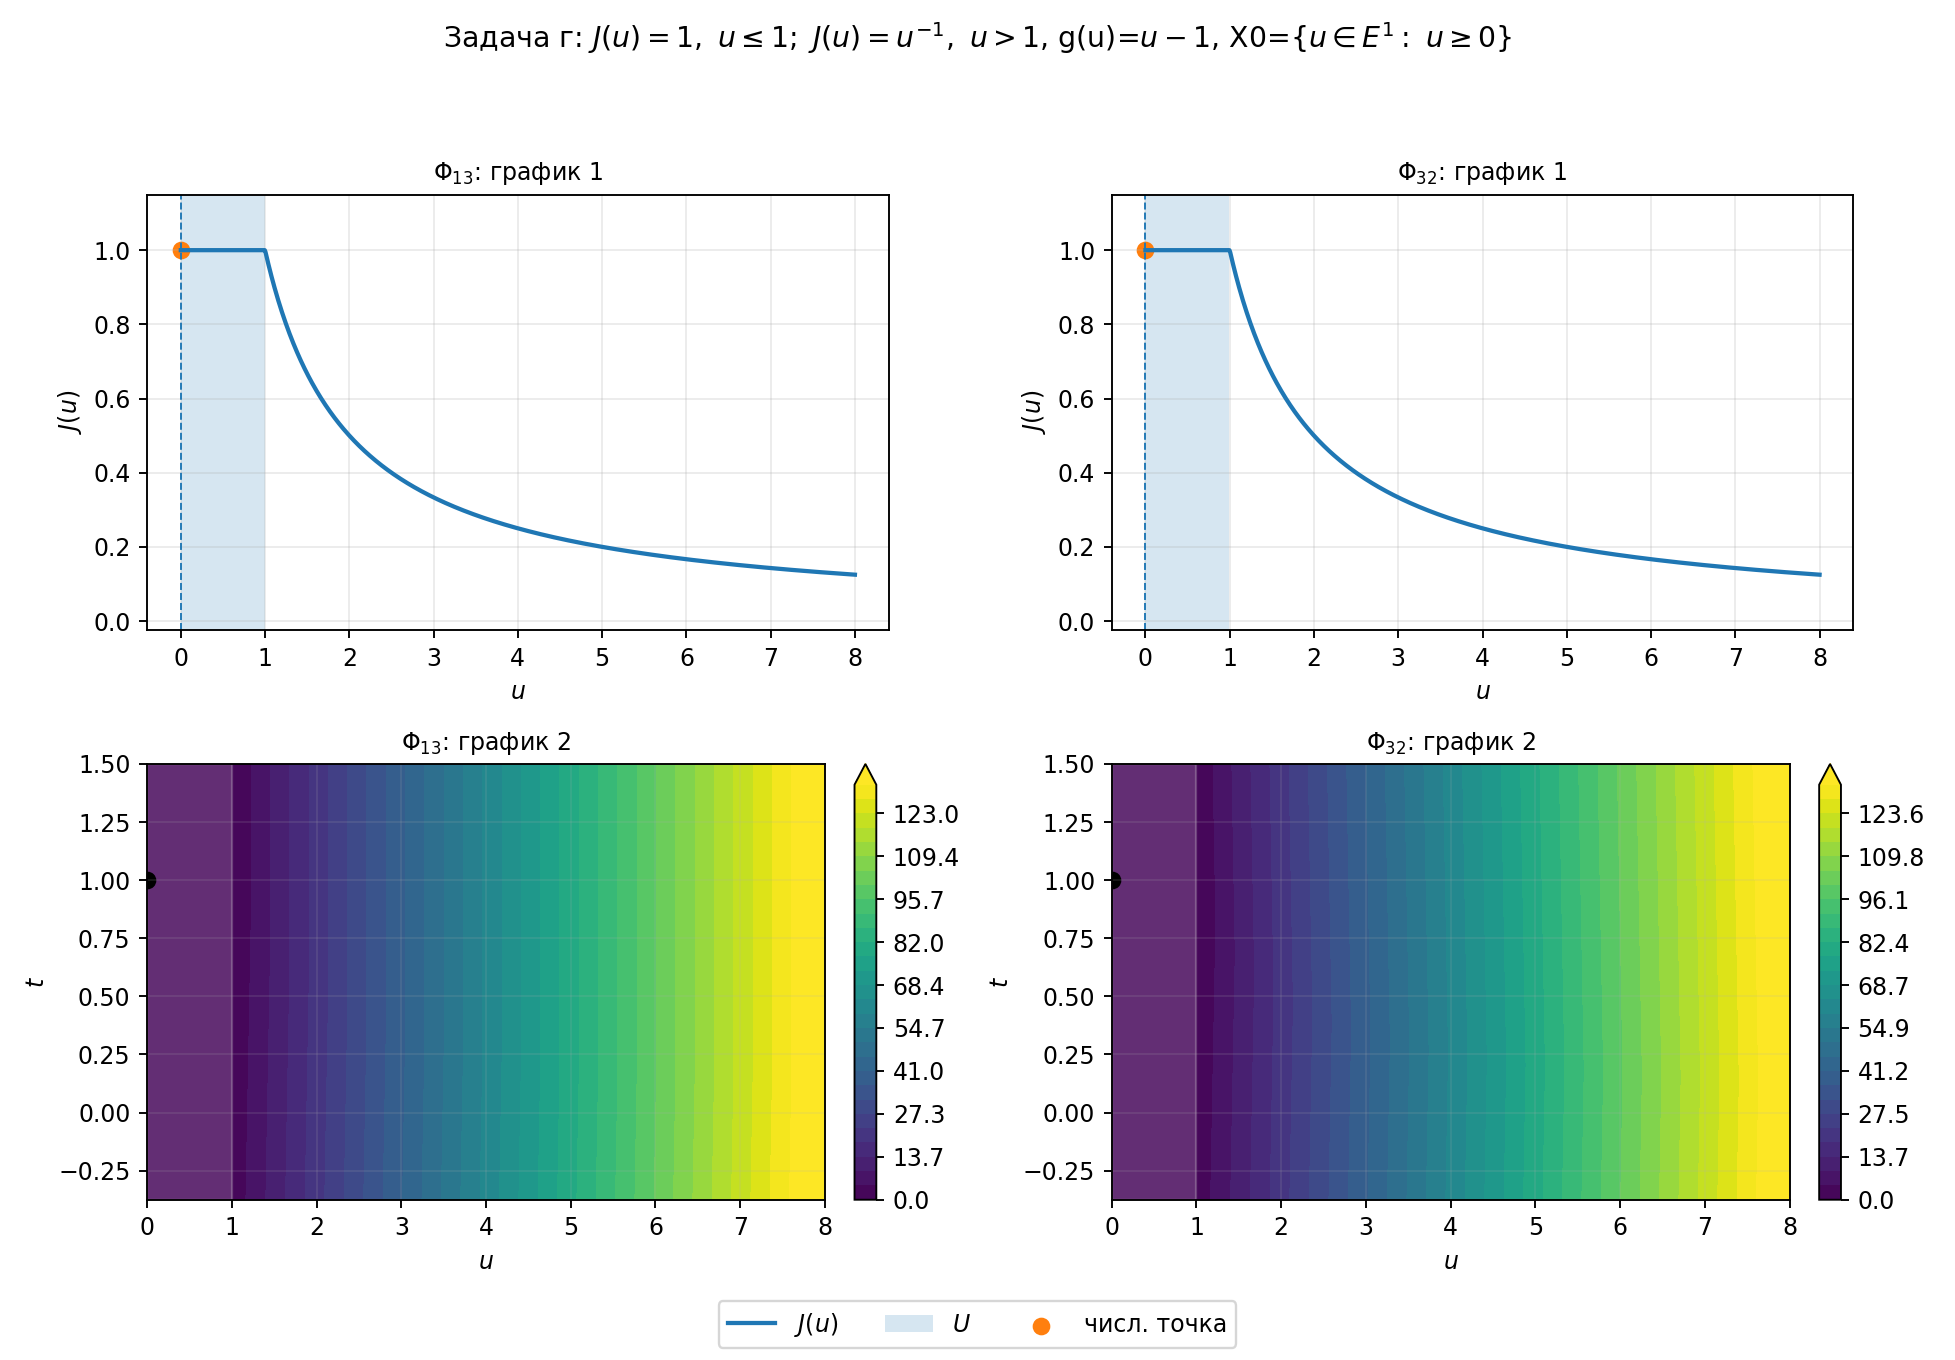
\includegraphics[width=0.96\textwidth]{graphs/g_g1_xge0_overview.png}
\caption{Задача г, вариант g1: $g(u)=u-1$, $X_0=\{u\in E^1:\ u\geq 0\}$. Верхний ряд: график 1 для $\Phi_{13}$ и $\Phi_{32}$; нижний ряд: график 2 для $\Phi_{13}$ и $\Phi_{32}$.}
\end{figure}

\begin{figure}[H]
\centering
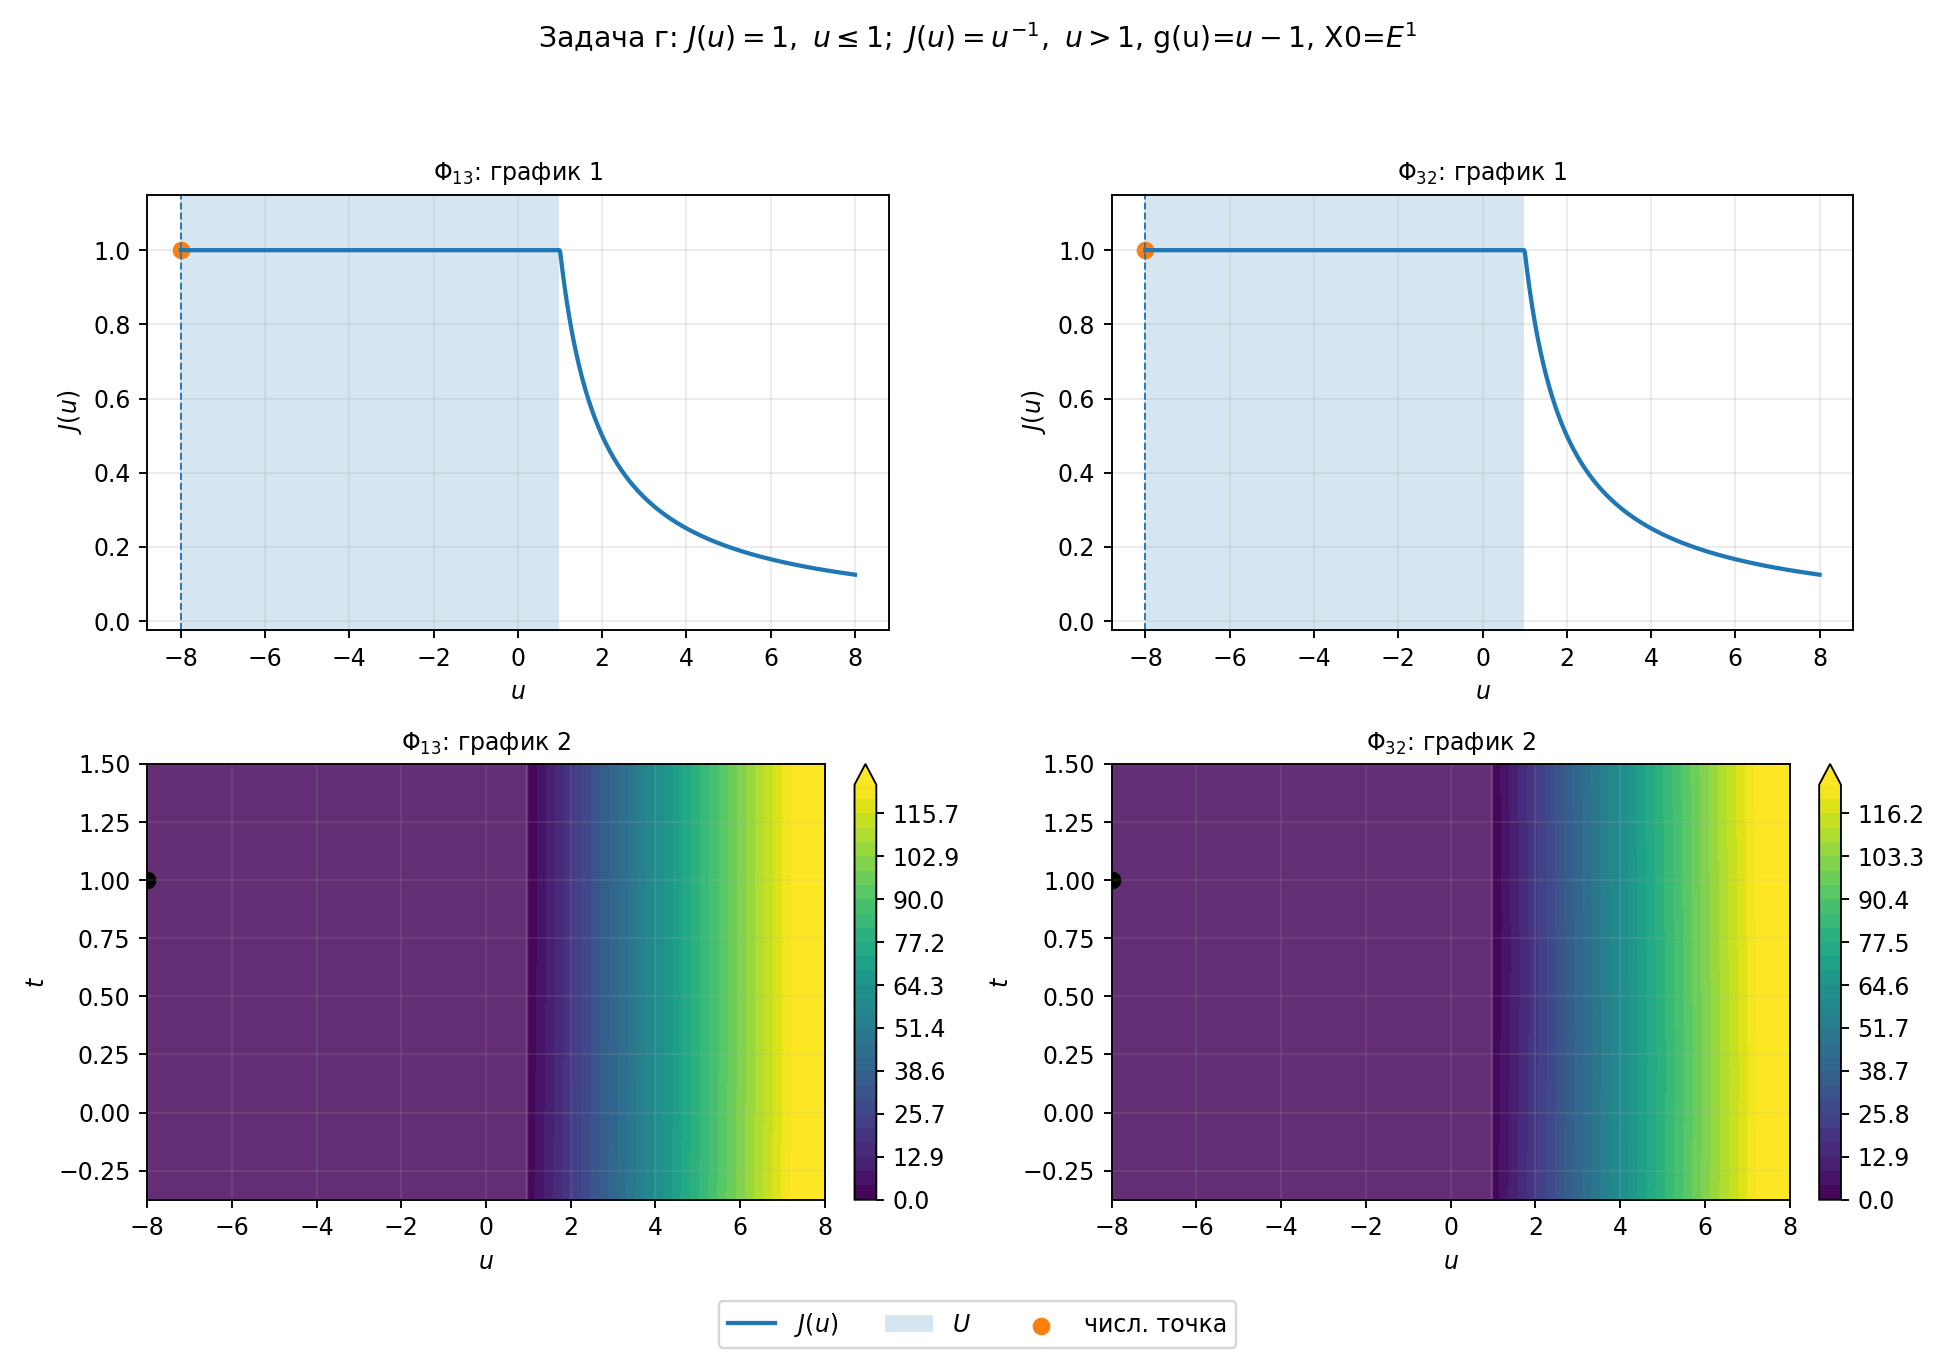
\includegraphics[width=0.96\textwidth]{graphs/g_g1_R_overview.png}
\caption{Задача г, вариант g1: $g(u)=u-1$, $X_0=E^1$. Верхний ряд: график 1 для $\Phi_{13}$ и $\Phi_{32}$; нижний ряд: график 2 для $\Phi_{13}$ и $\Phi_{32}$.}
\end{figure}

\begin{figure}[H]
\centering
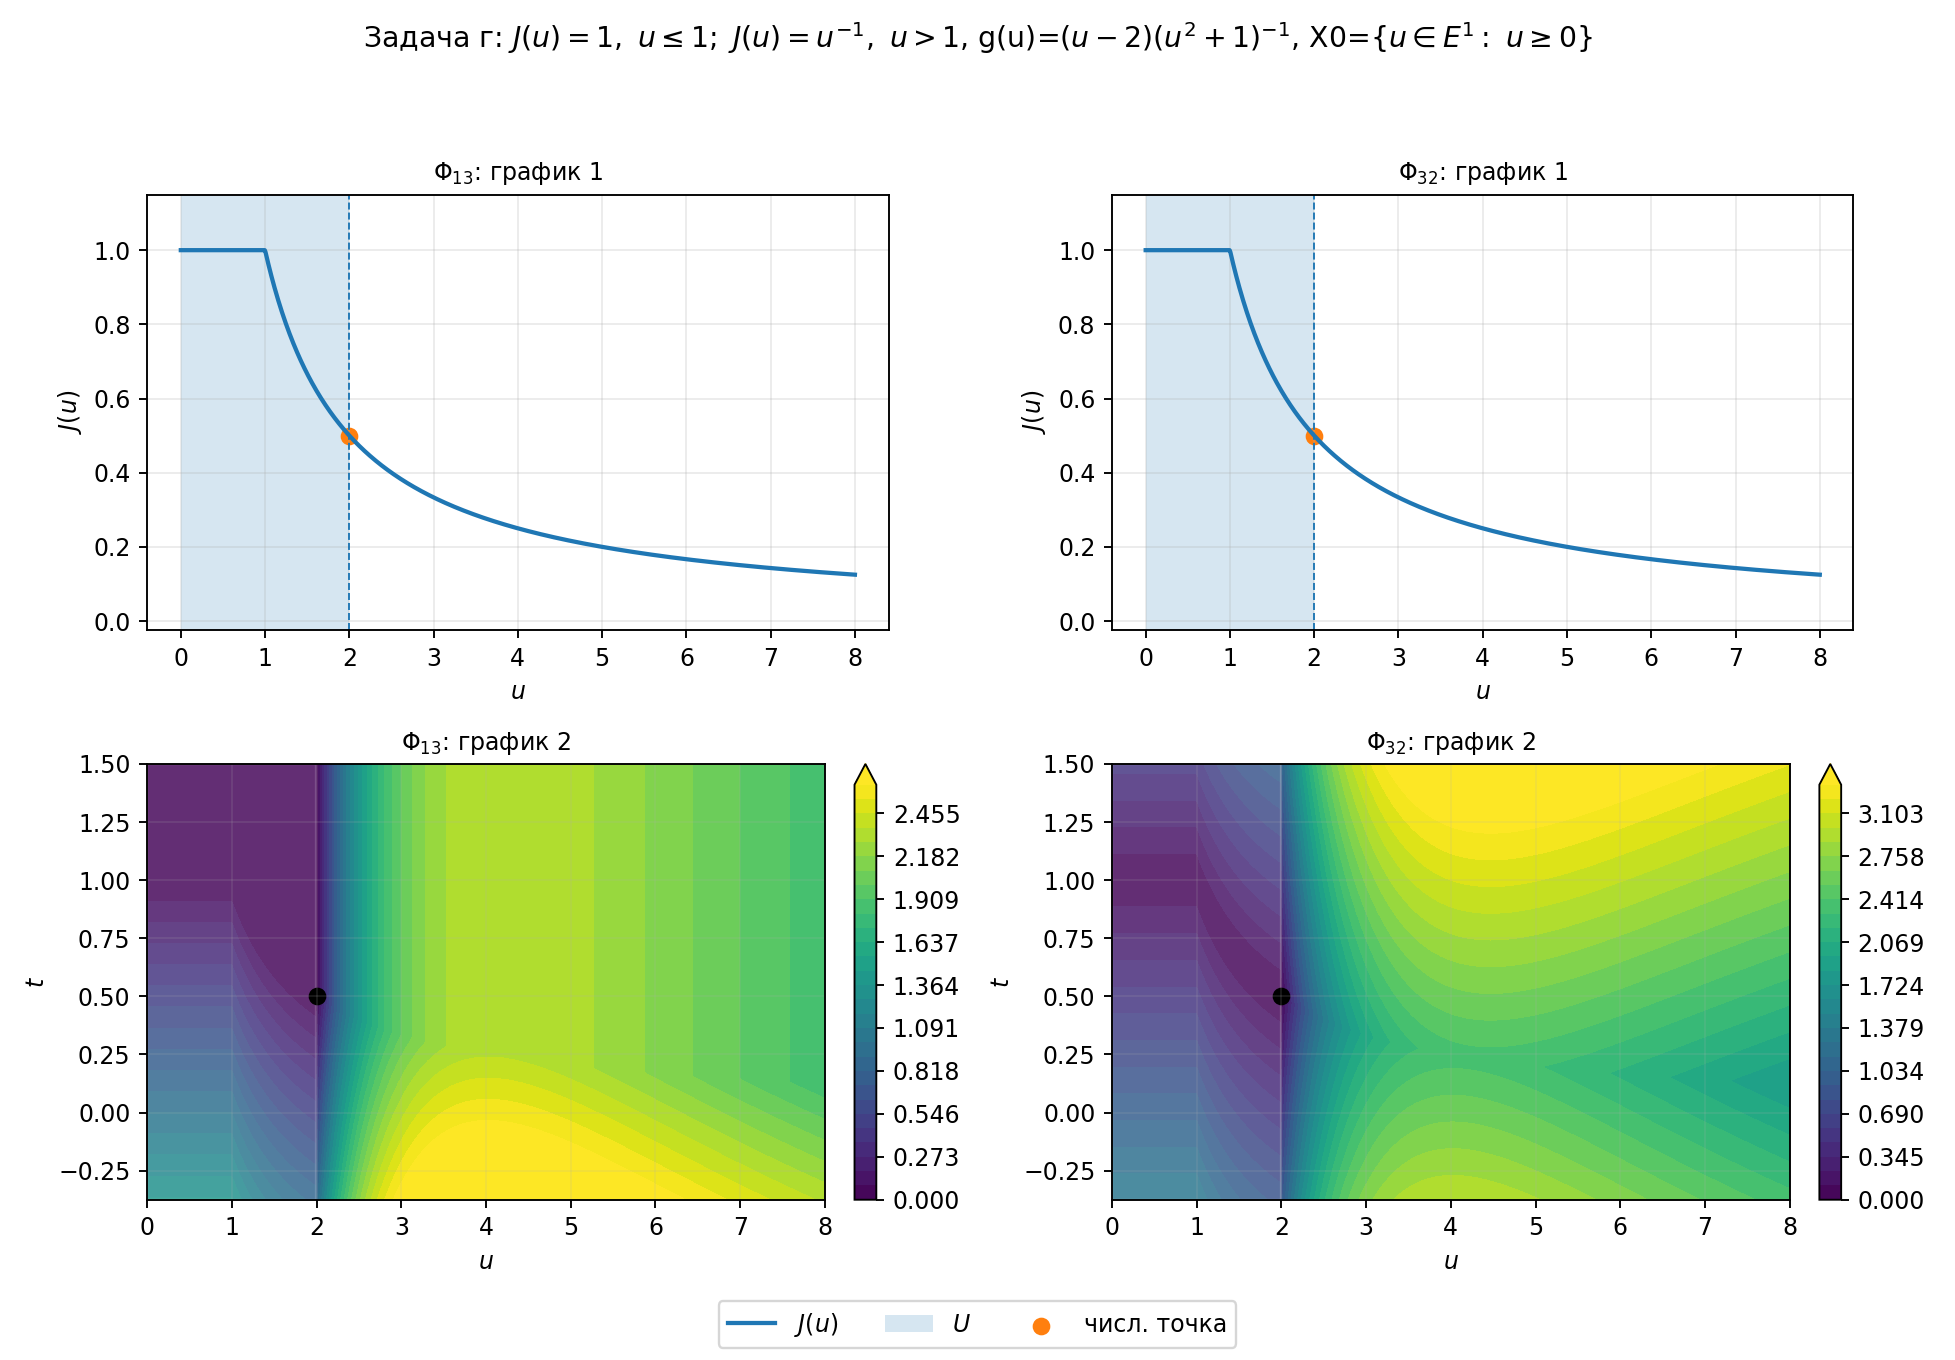
\includegraphics[width=0.96\textwidth]{graphs/g_g2_xge0_overview.png}
\caption{Задача г, вариант g2: $g(u)=(u-2)(u^2+1)^{-1}$, $X_0=\{u\in E^1:\ u\geq 0\}$. Верхний ряд: график 1 для $\Phi_{13}$ и $\Phi_{32}$; нижний ряд: график 2 для $\Phi_{13}$ и $\Phi_{32}$.}
\end{figure}

\begin{figure}[H]
\centering
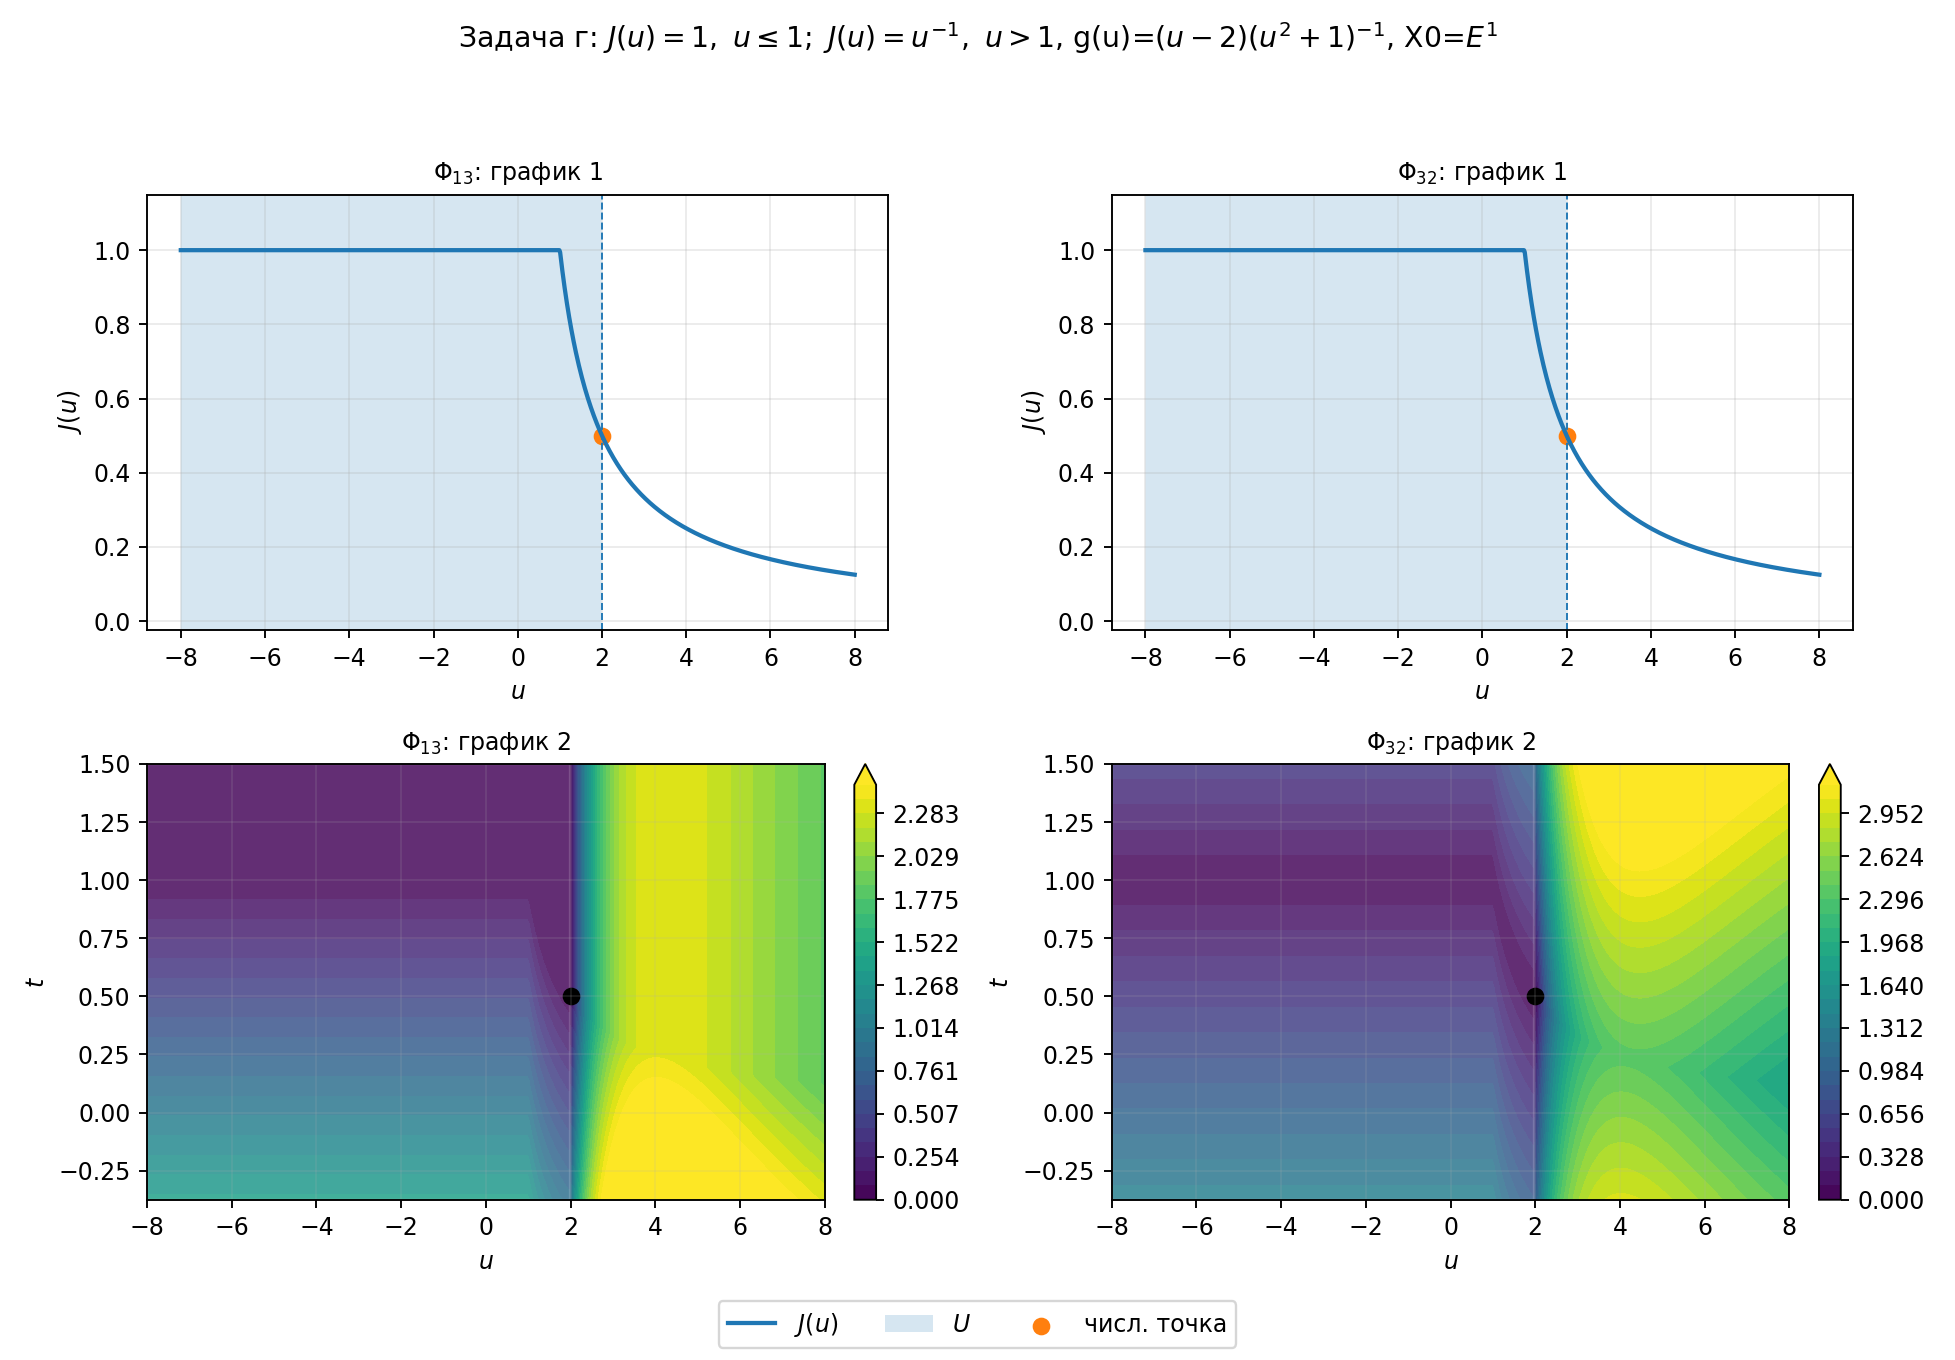
\includegraphics[width=0.96\textwidth]{graphs/g_g2_R_overview.png}
\caption{Задача г, вариант g2: $g(u)=(u-2)(u^2+1)^{-1}$, $X_0=E^1$. Верхний ряд: график 1 для $\Phi_{13}$ и $\Phi_{32}$; нижний ряд: график 2 для $\Phi_{13}$ и $\Phi_{32}$.}
\end{figure}

\begin{figure}[H]
\centering
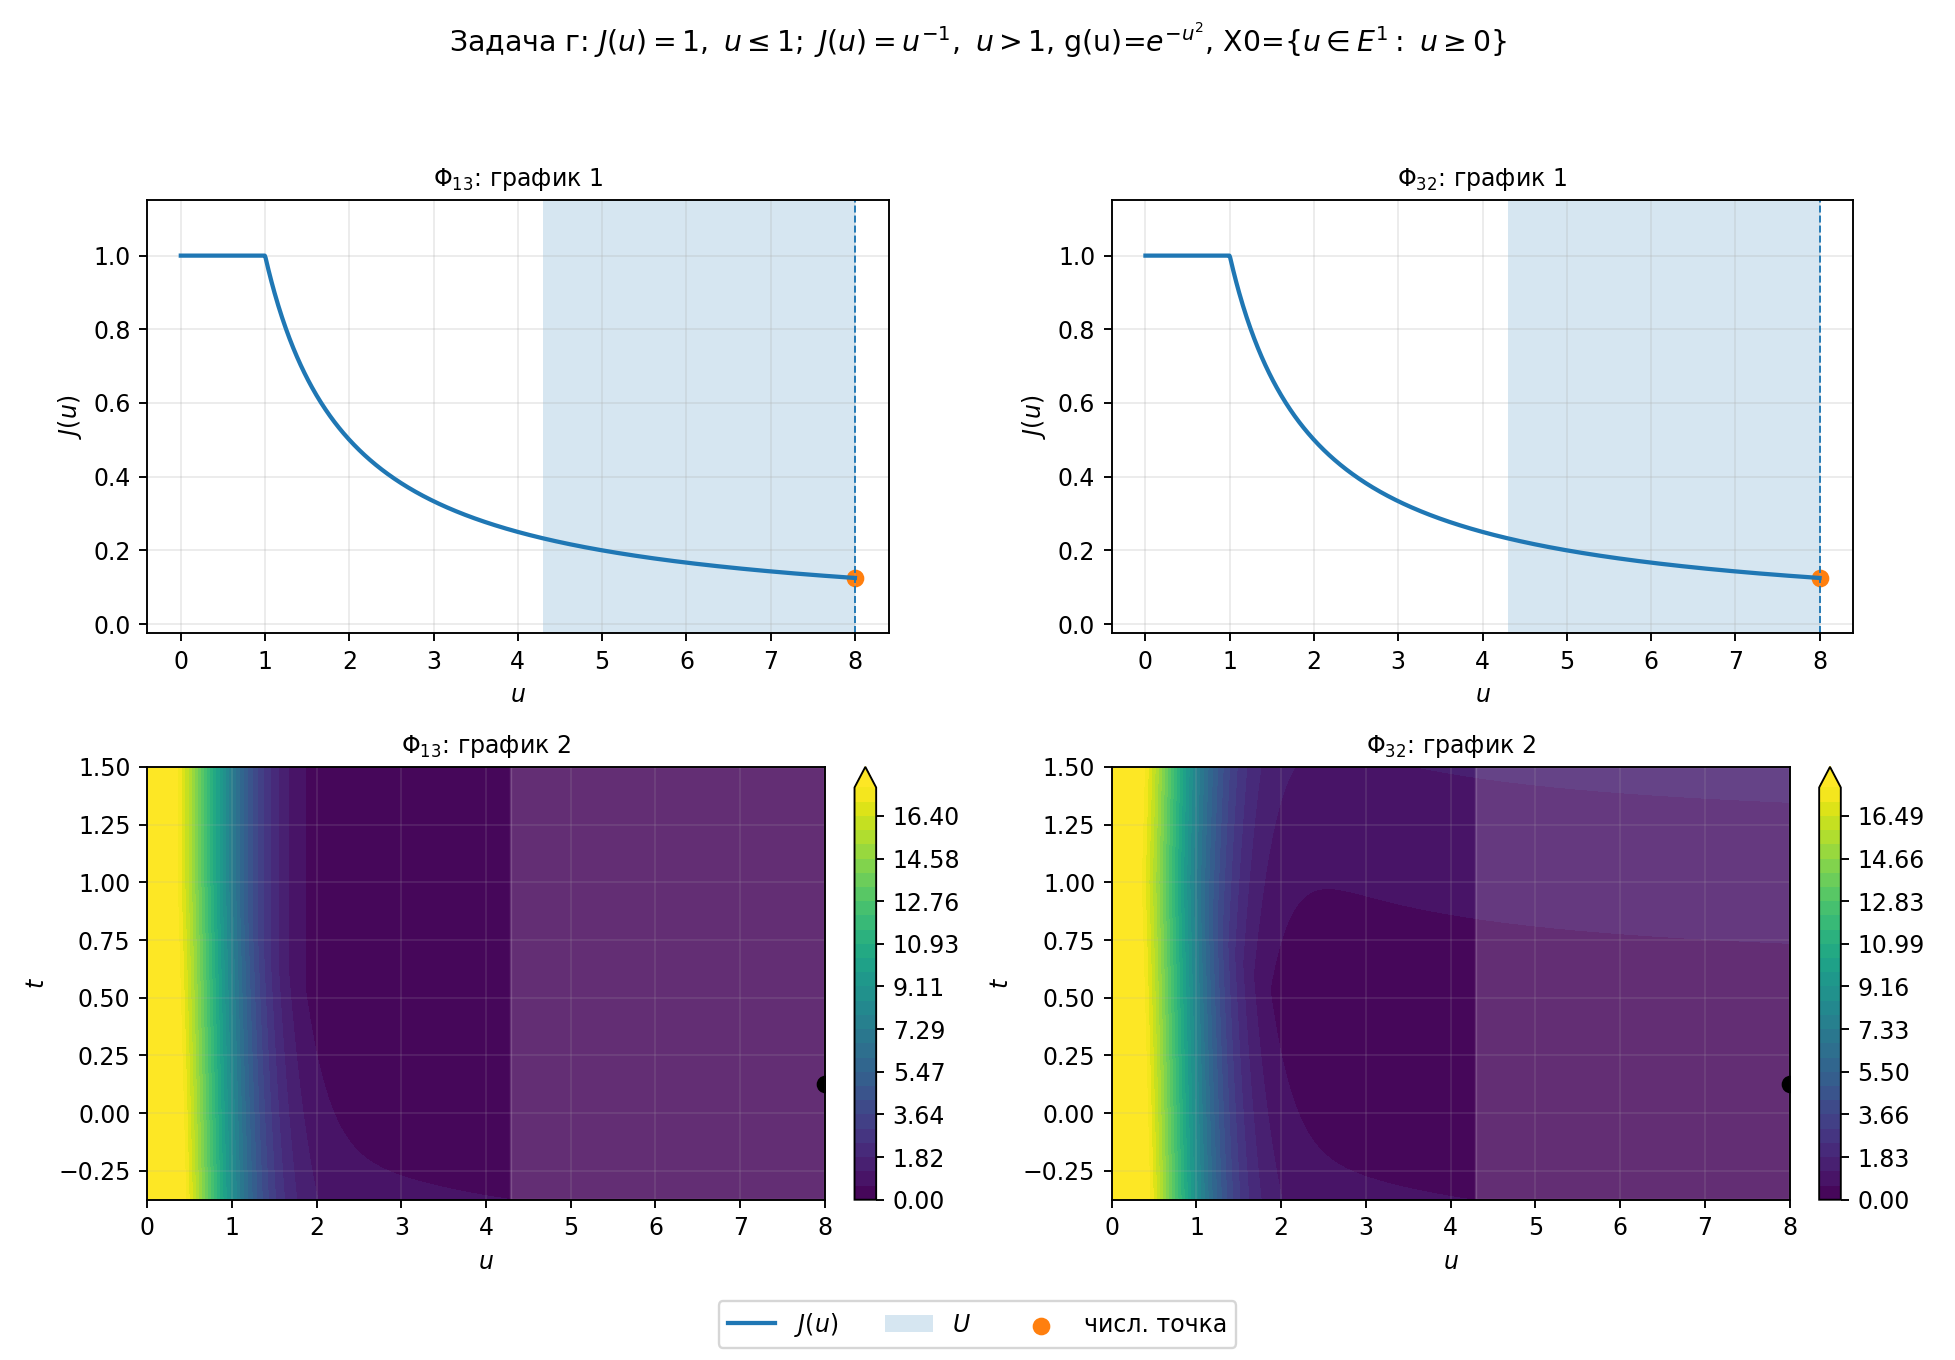
\includegraphics[width=0.96\textwidth]{graphs/g_g3_xge0_overview.png}
\caption{Задача г, вариант g3: $g(u)=e^{-u^2}$, $X_0=\{u\in E^1:\ u\geq 0\}$. Верхний ряд: график 1 для $\Phi_{13}$ и $\Phi_{32}$; нижний ряд: график 2 для $\Phi_{13}$ и $\Phi_{32}$.}
\end{figure}

\begin{figure}[H]
\centering
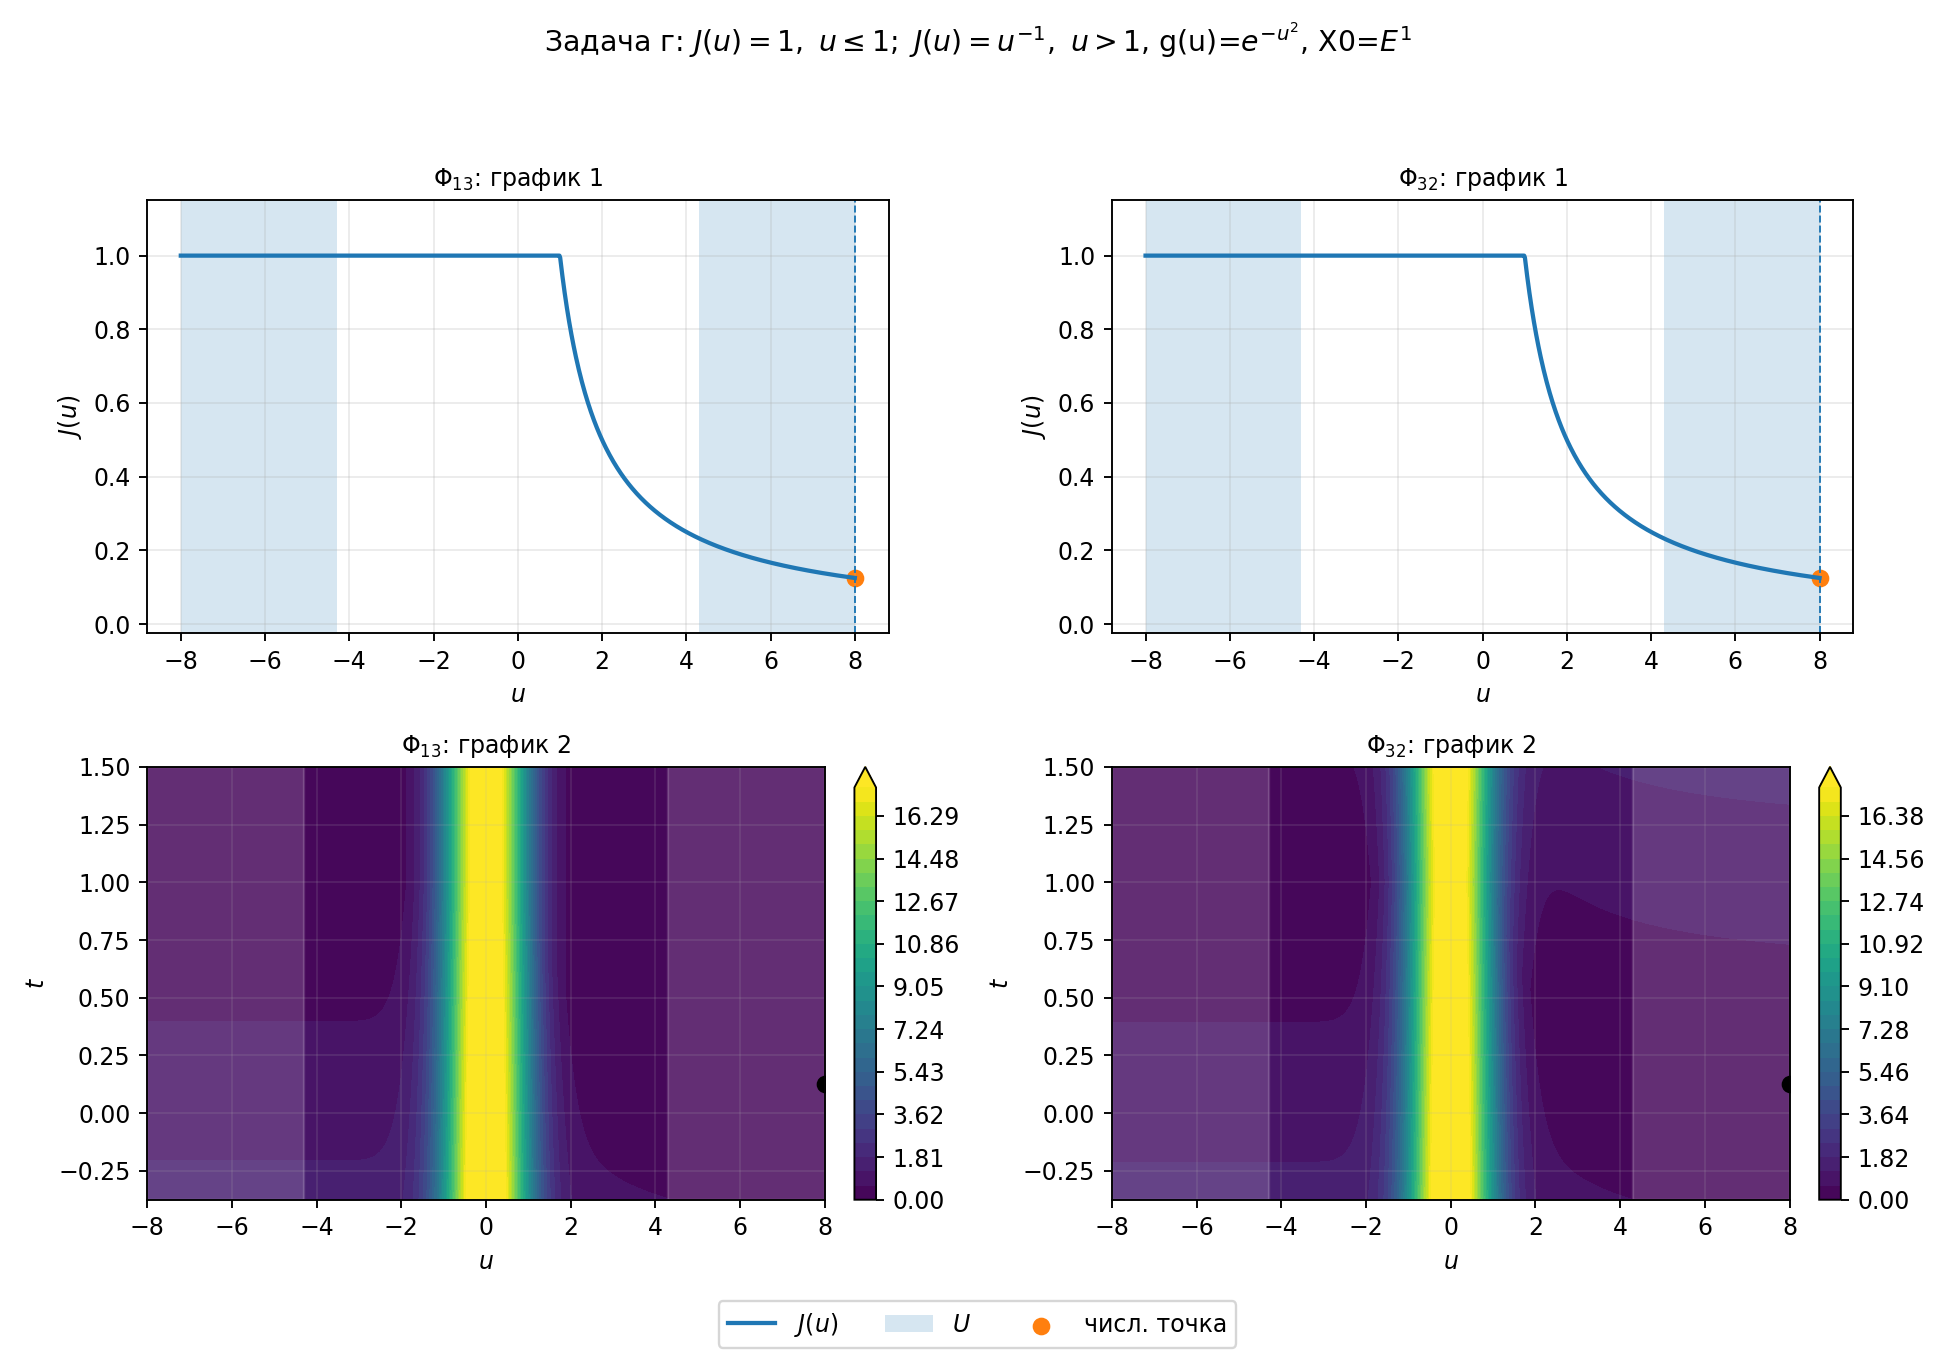
\includegraphics[width=0.96\textwidth]{graphs/g_g3_R_overview.png}
\caption{Задача г, вариант g3: $g(u)=e^{-u^2}$, $X_0=E^1$. Верхний ряд: график 1 для $\Phi_{13}$ и $\Phi_{32}$; нижний ряд: график 2 для $\Phi_{13}$ и $\Phi_{32}$.}
\end{figure}

\begin{figure}[H]
\centering
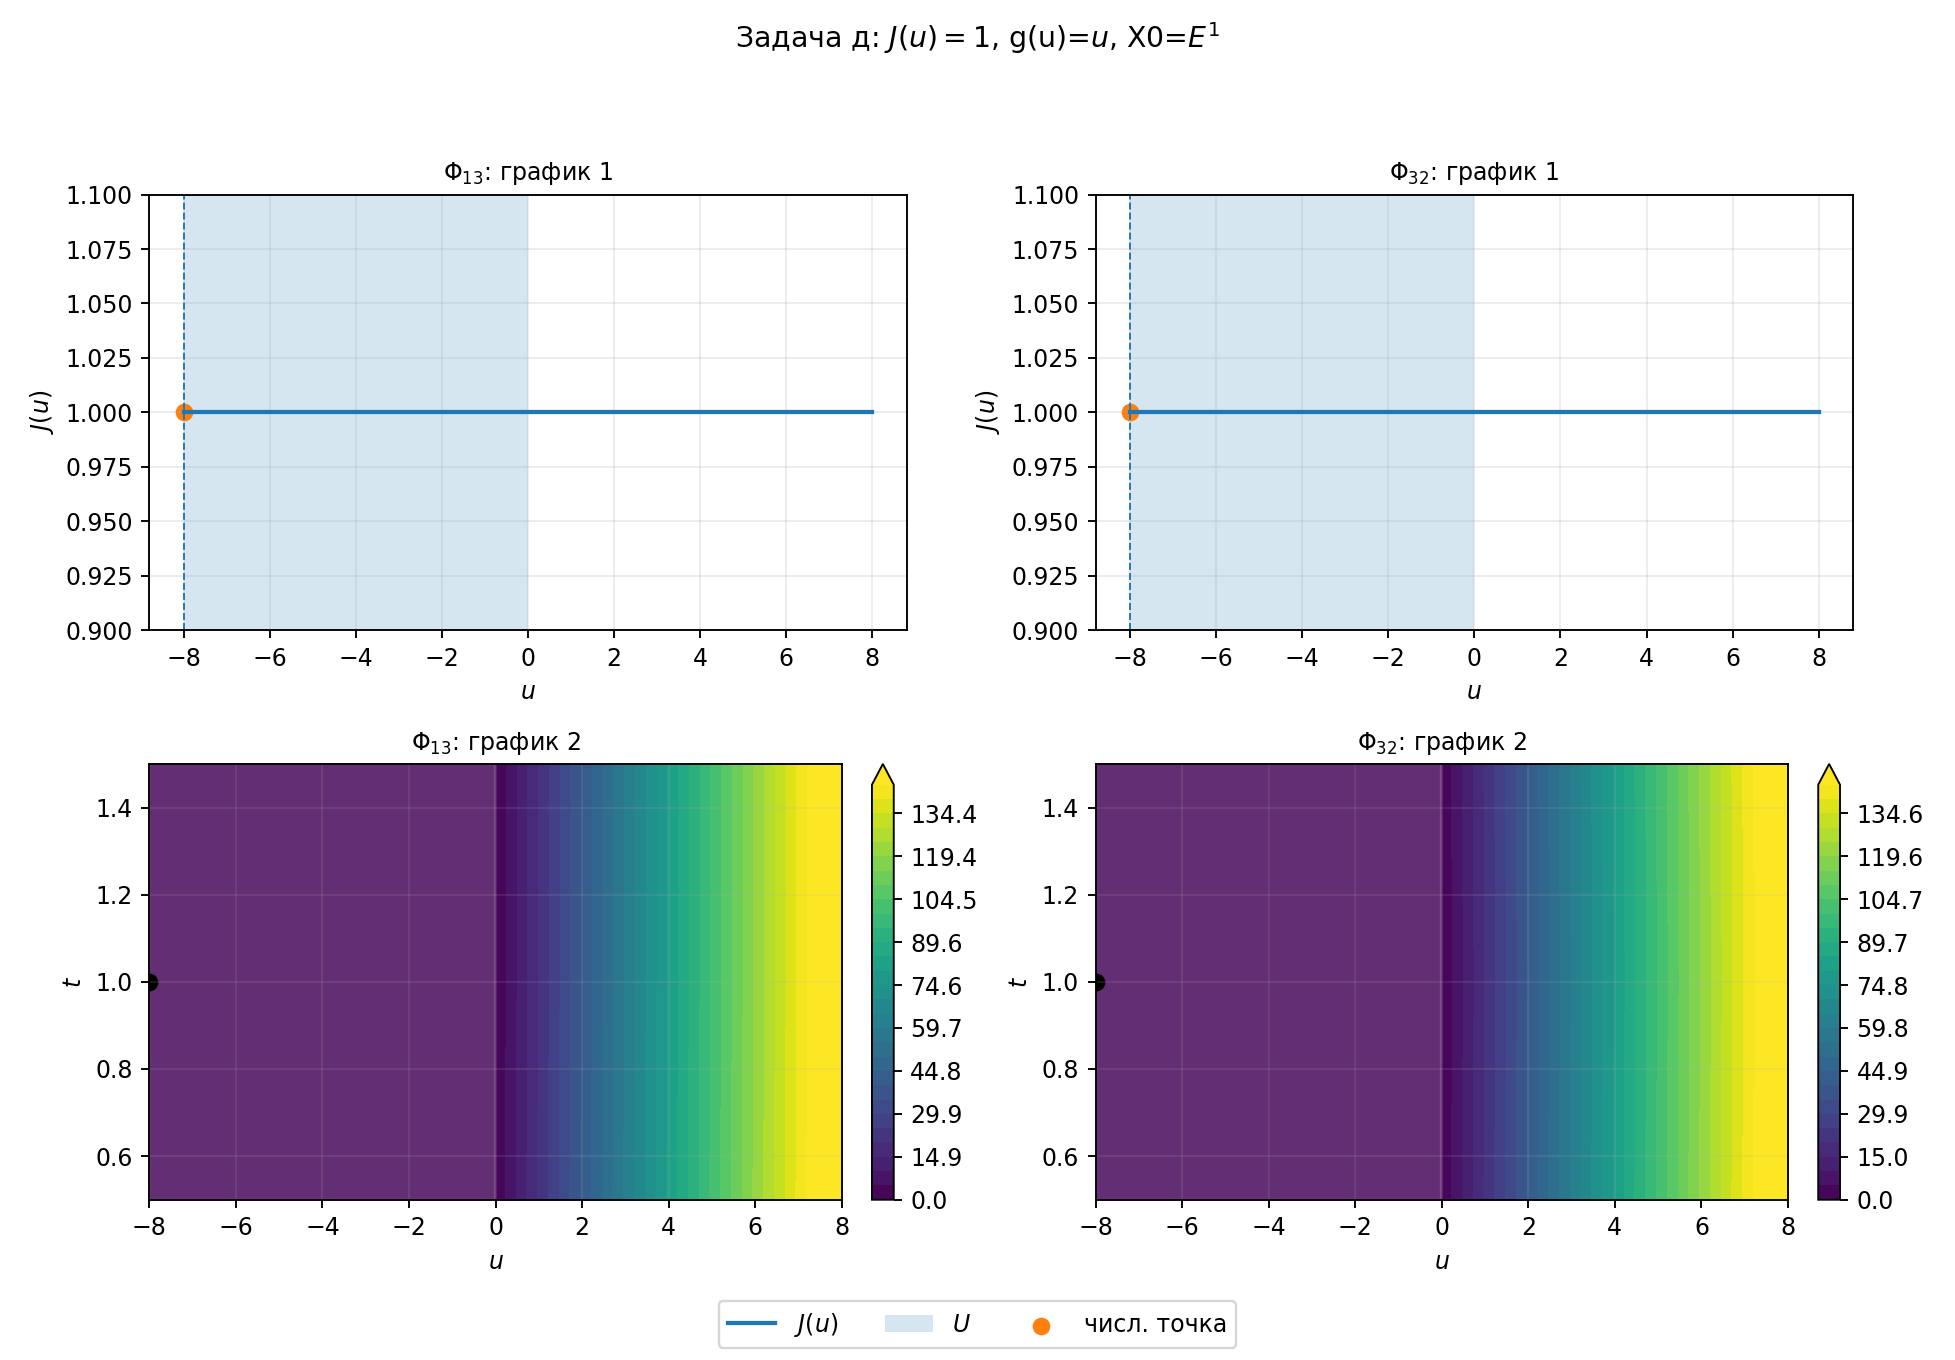
\includegraphics[width=0.96\textwidth]{graphs/d_g1_R_overview.png}
\caption{Задача д, вариант g1: $g(u)=u$, $X_0=E^1$. Верхний ряд: график 1 для $\Phi_{13}$ и $\Phi_{32}$; нижний ряд: график 2 для $\Phi_{13}$ и $\Phi_{32}$.}
\end{figure}

\begin{figure}[H]
\centering
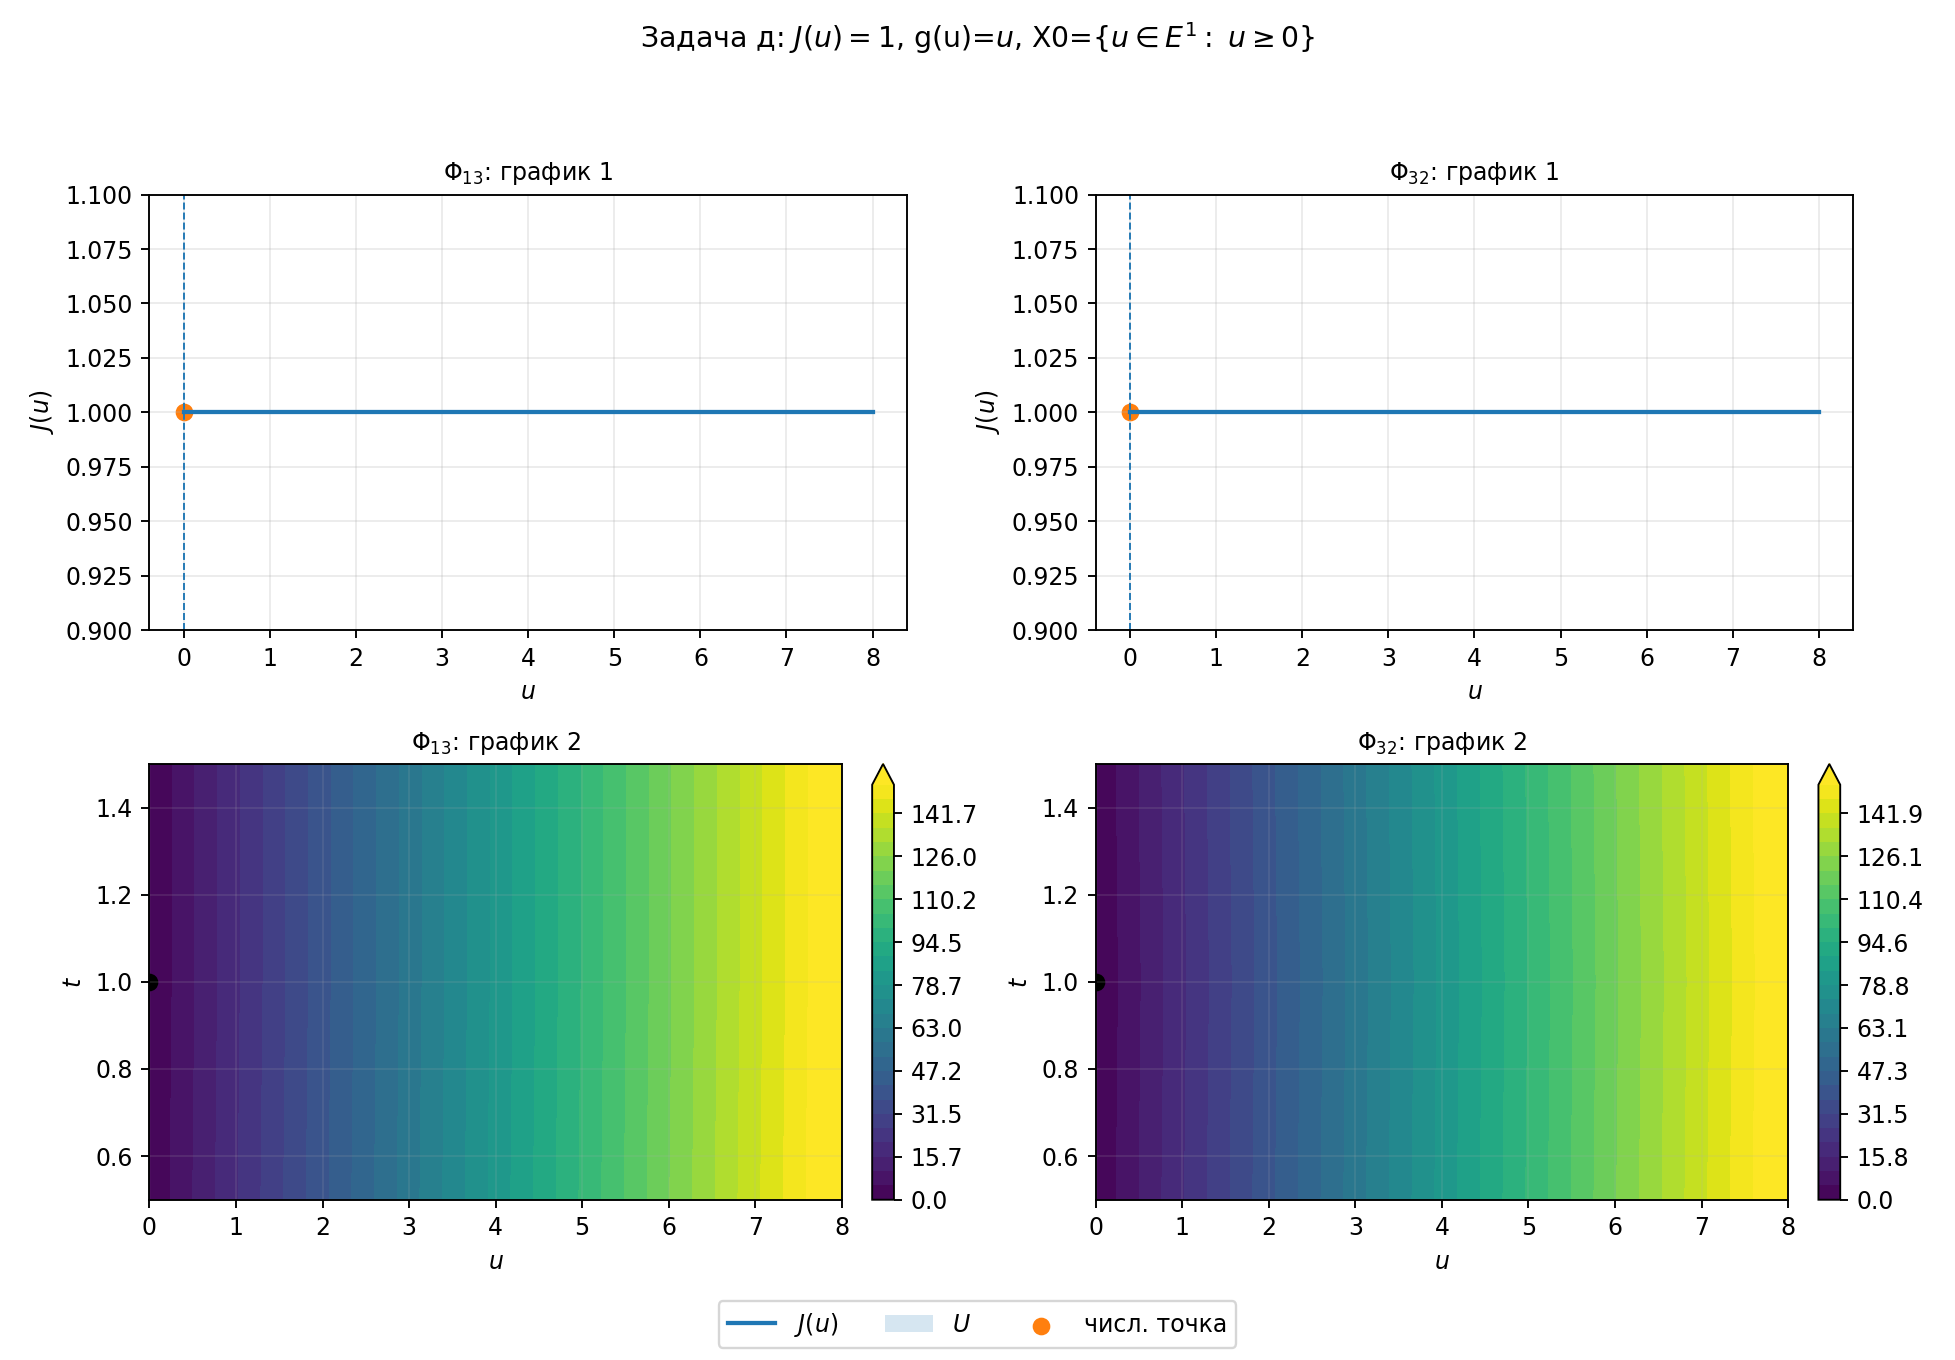
\includegraphics[width=0.96\textwidth]{graphs/d_g1_xge0_overview.png}
\caption{Задача д, вариант g1: $g(u)=u$, $X_0=\{u\in E^1:\ u\geq 0\}$. Верхний ряд: график 1 для $\Phi_{13}$ и $\Phi_{32}$; нижний ряд: график 2 для $\Phi_{13}$ и $\Phi_{32}$.}
\end{figure}

\begin{figure}[H]
\centering
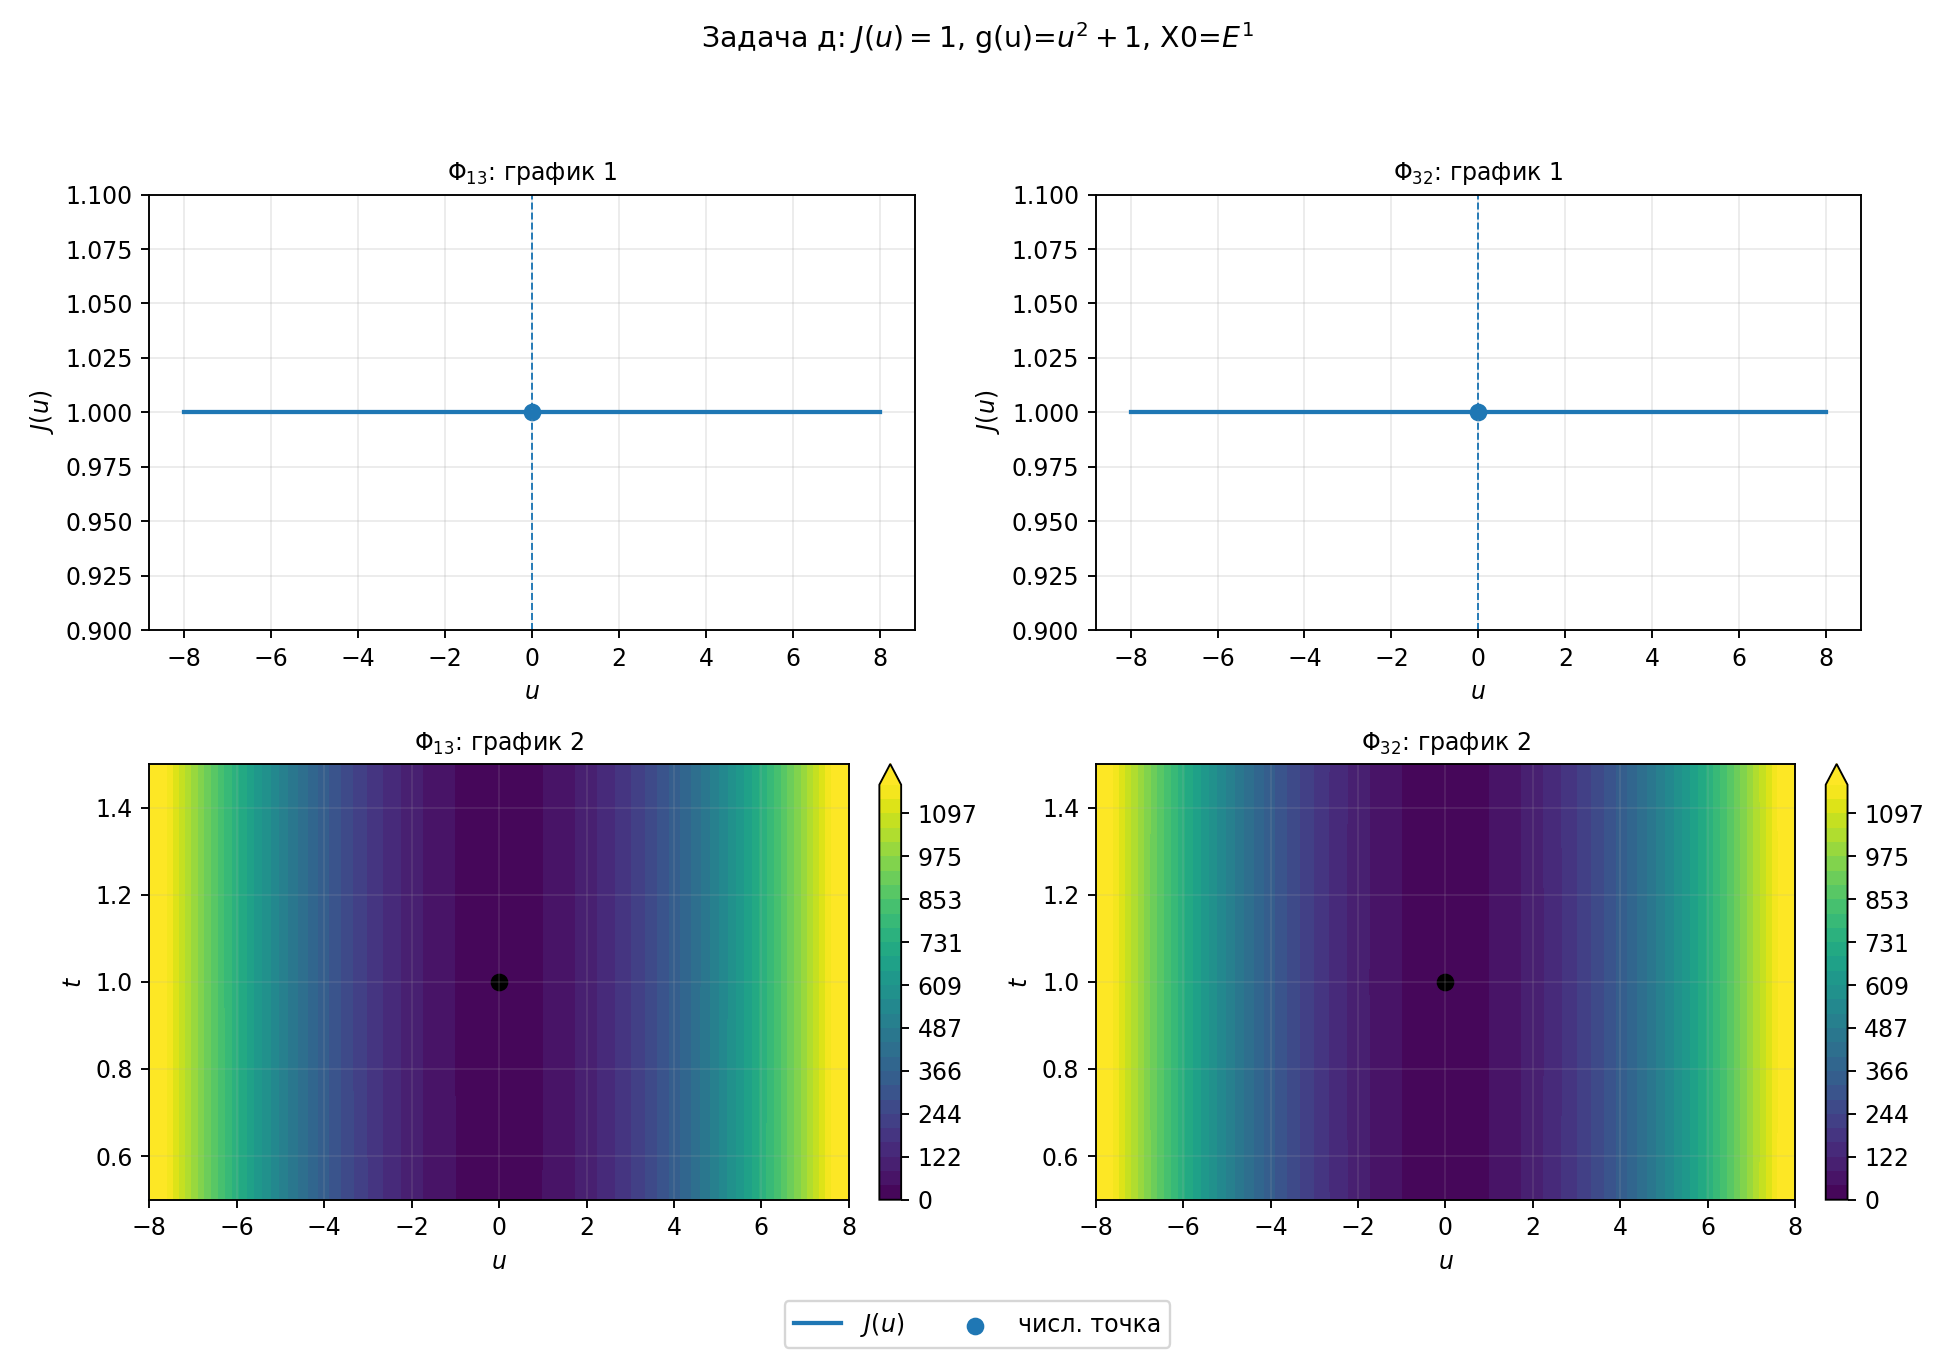
\includegraphics[width=0.96\textwidth]{graphs/d_g2_R_overview.png}
\caption{Задача д, вариант g2: $g(u)=u^2+1$, $X_0=E^1$. Верхний ряд: график 1 для $\Phi_{13}$ и $\Phi_{32}$; нижний ряд: график 2 для $\Phi_{13}$ и $\Phi_{32}$.}
\end{figure}

\begin{figure}[H]
\centering
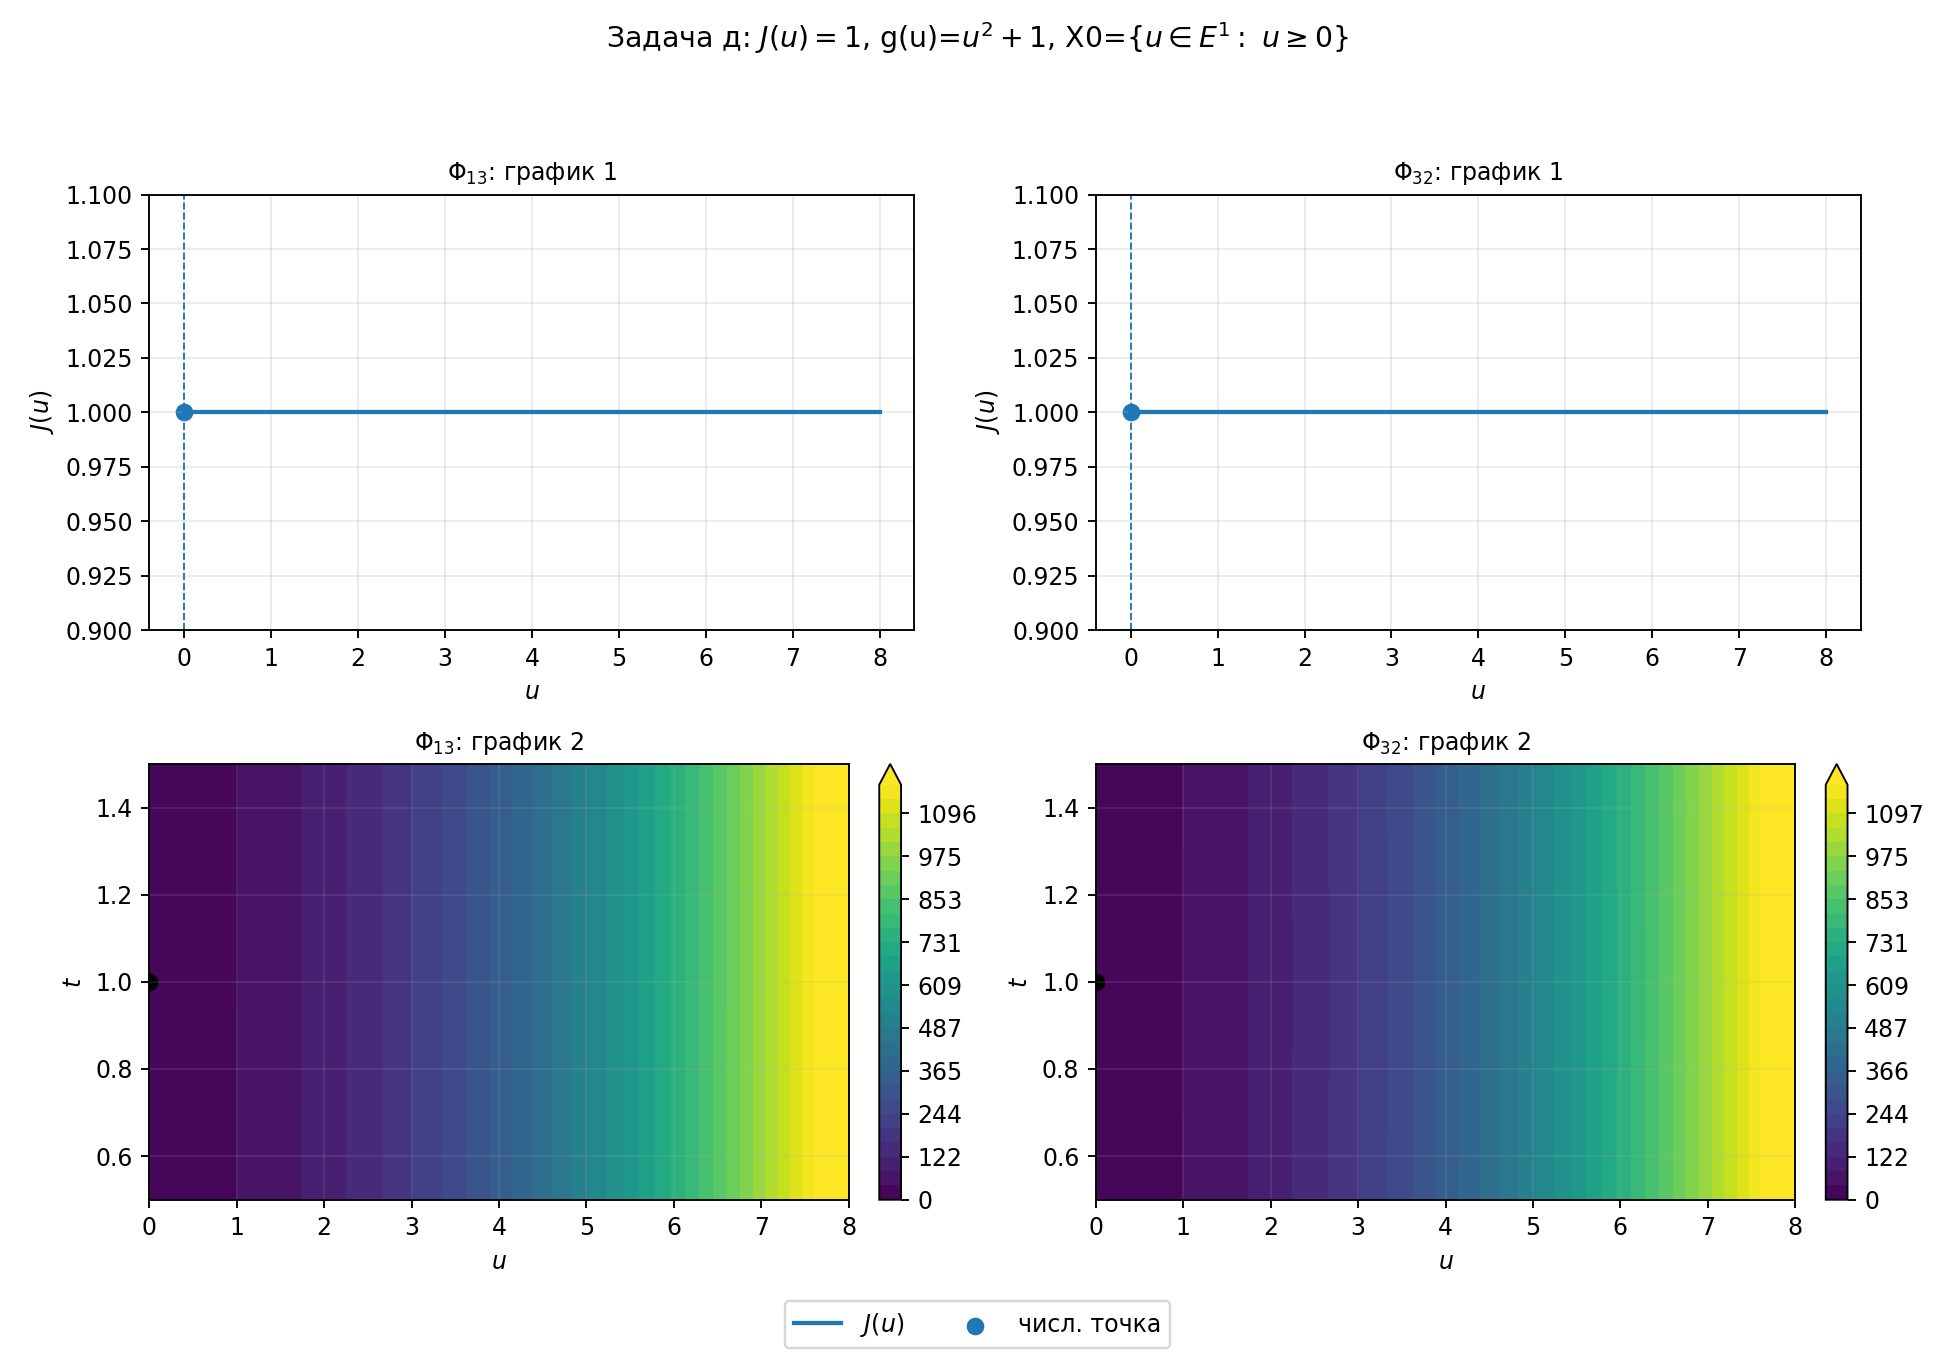
\includegraphics[width=0.96\textwidth]{graphs/d_g2_xge0_overview.png}
\caption{Задача д, вариант g2: $g(u)=u^2+1$, $X_0=\{u\in E^1:\ u\geq 0\}$. Верхний ряд: график 1 для $\Phi_{13}$ и $\Phi_{32}$; нижний ряд: график 2 для $\Phi_{13}$ и $\Phi_{32}$.}
\end{figure}

\begin{figure}[H]
\centering
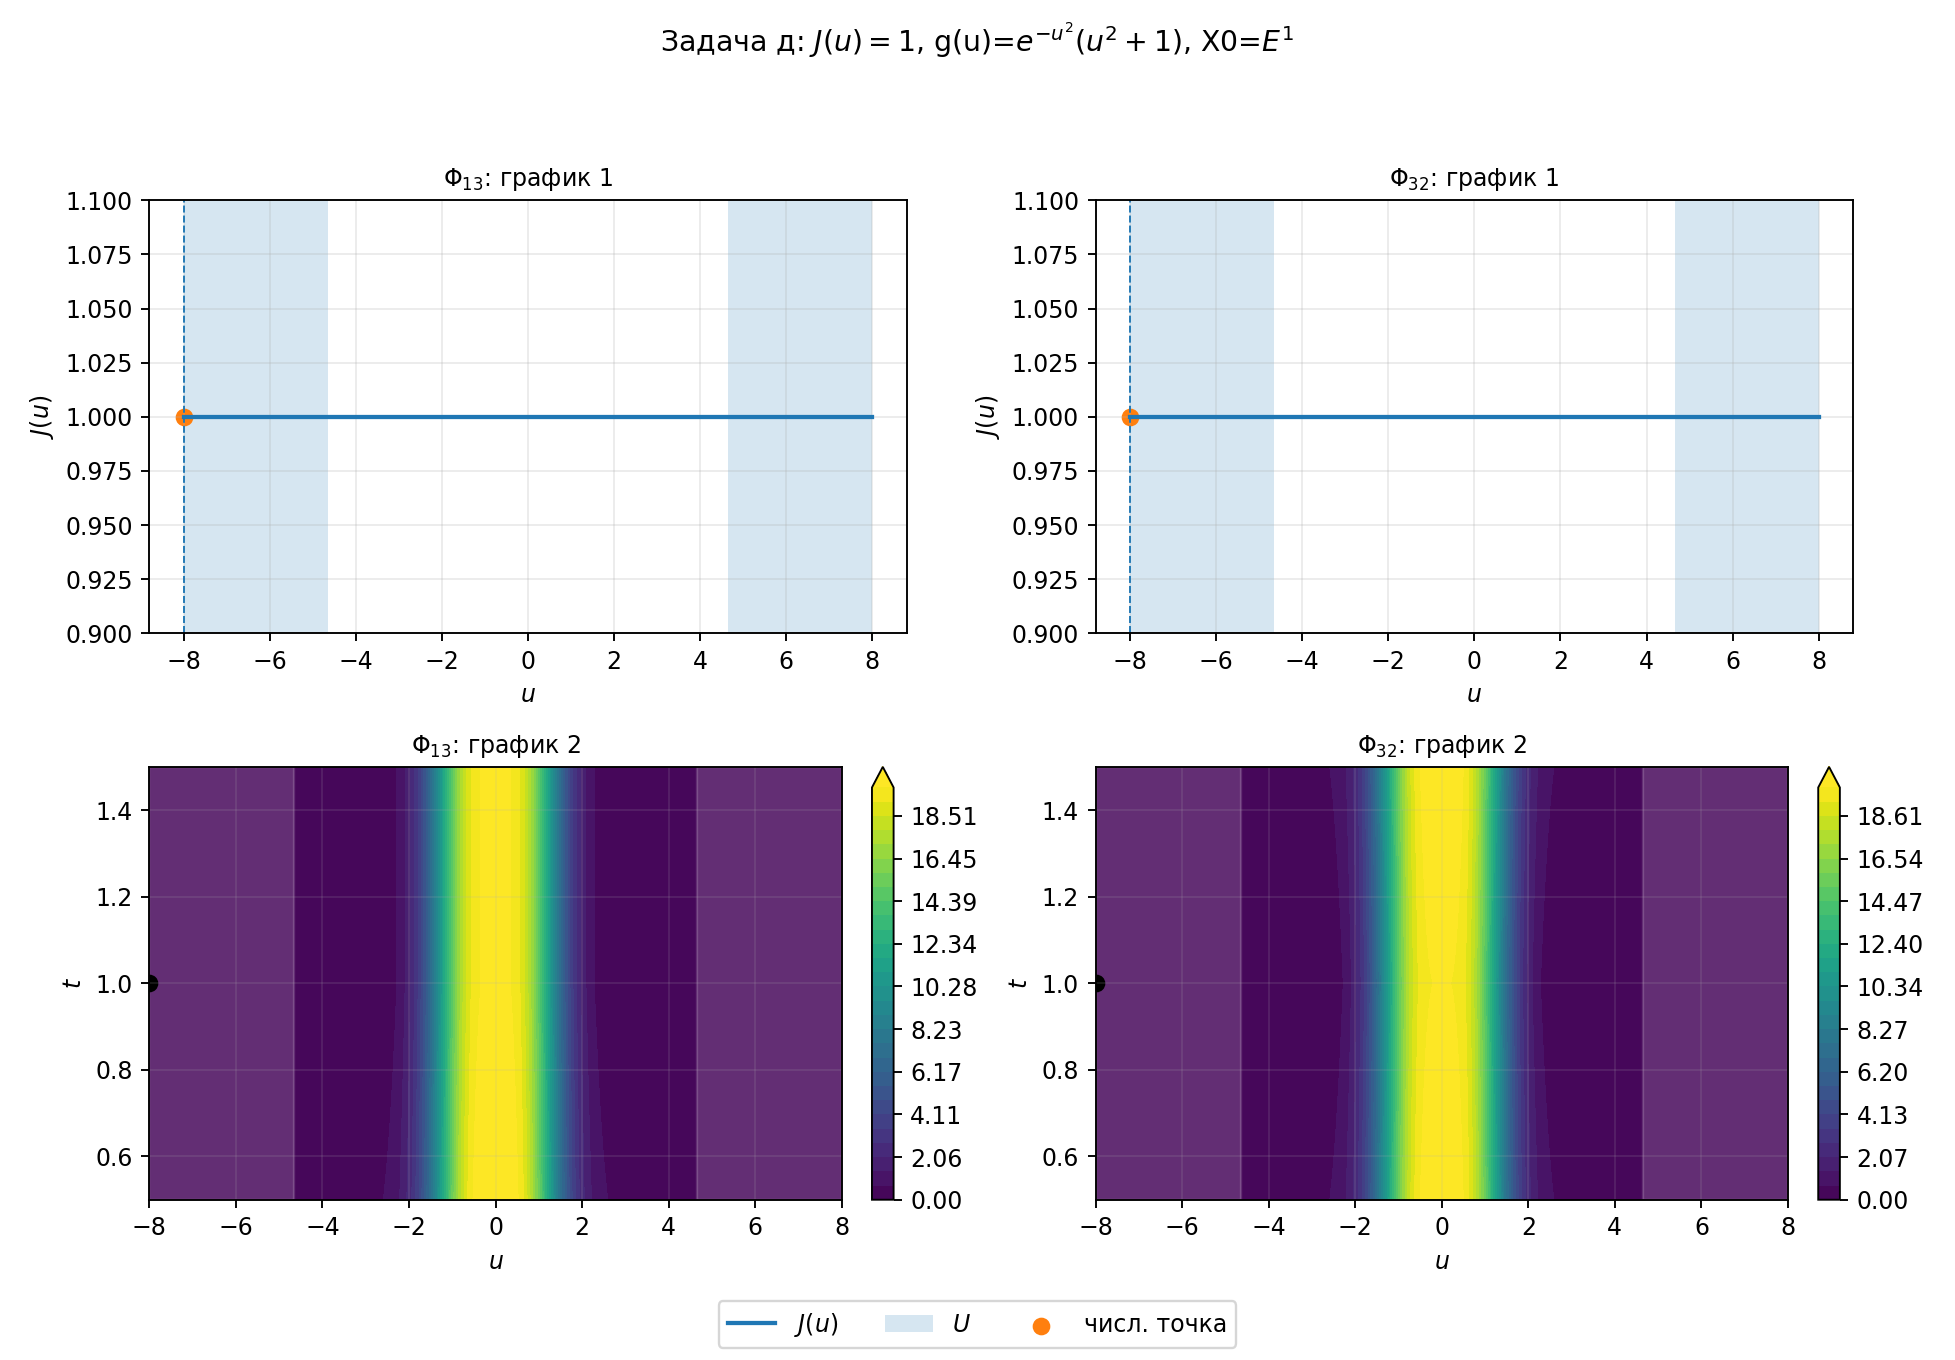
\includegraphics[width=0.96\textwidth]{graphs/d_g3_R_overview.png}
\caption{Задача д, вариант g3: $g(u)=e^{-u^2}(u^2+1)$, $X_0=E^1$. Верхний ряд: график 1 для $\Phi_{13}$ и $\Phi_{32}$; нижний ряд: график 2 для $\Phi_{13}$ и $\Phi_{32}$.}
\end{figure}

\begin{figure}[H]
\centering
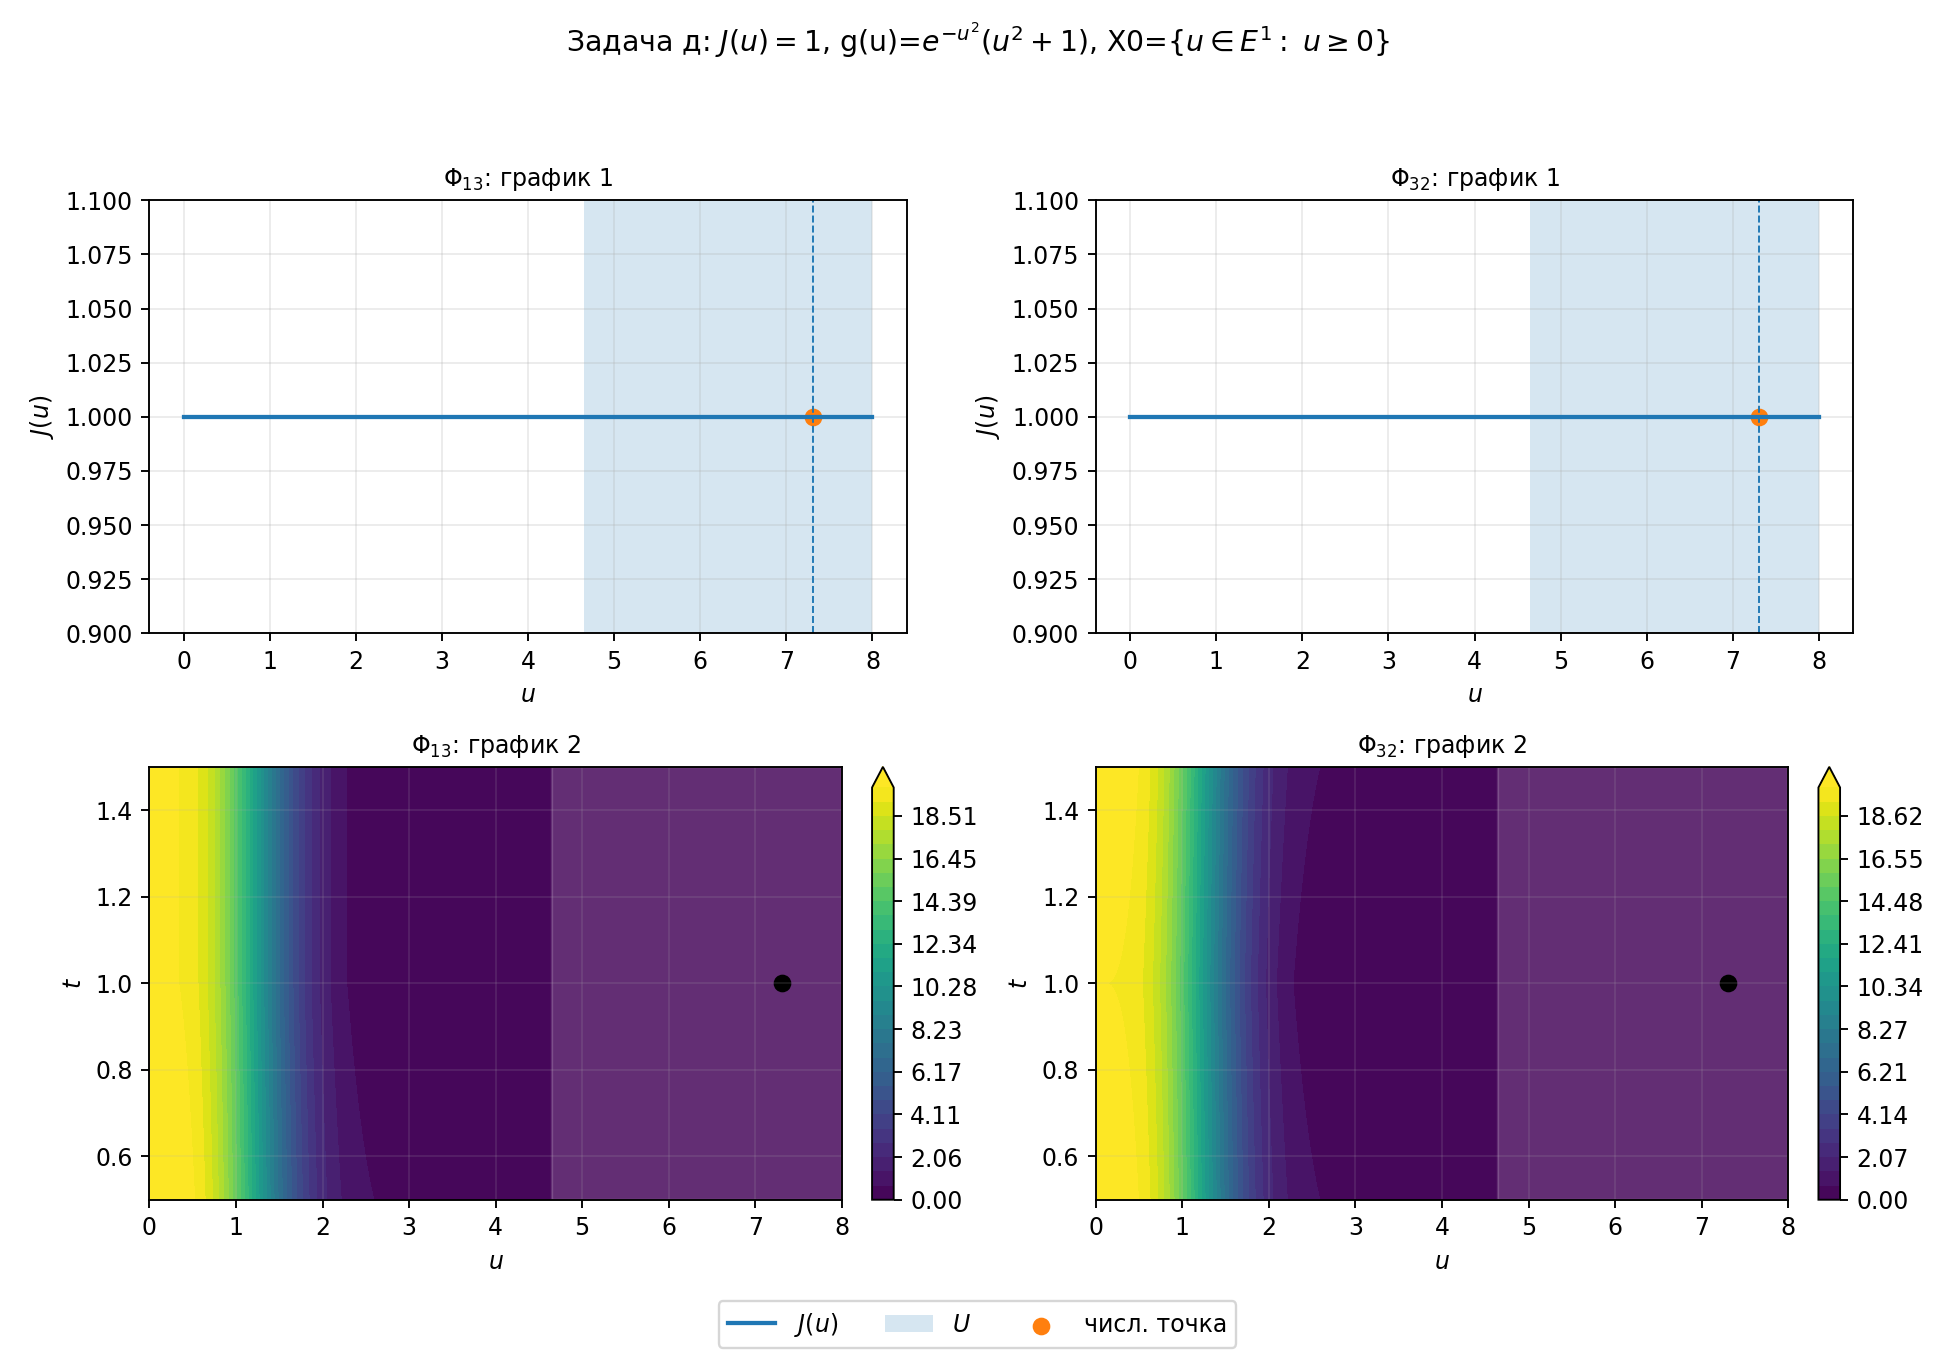
\includegraphics[width=0.96\textwidth]{graphs/d_g3_xge0_overview.png}
\caption{Задача д, вариант g3: $g(u)=e^{-u^2}(u^2+1)$, $X_0=\{u\in E^1:\ u\geq 0\}$. Верхний ряд: график 1 для $\Phi_{13}$ и $\Phi_{32}$; нижний ряд: график 2 для $\Phi_{13}$ и $\Phi_{32}$.}
\end{figure}

\begin{figure}[H]
\centering
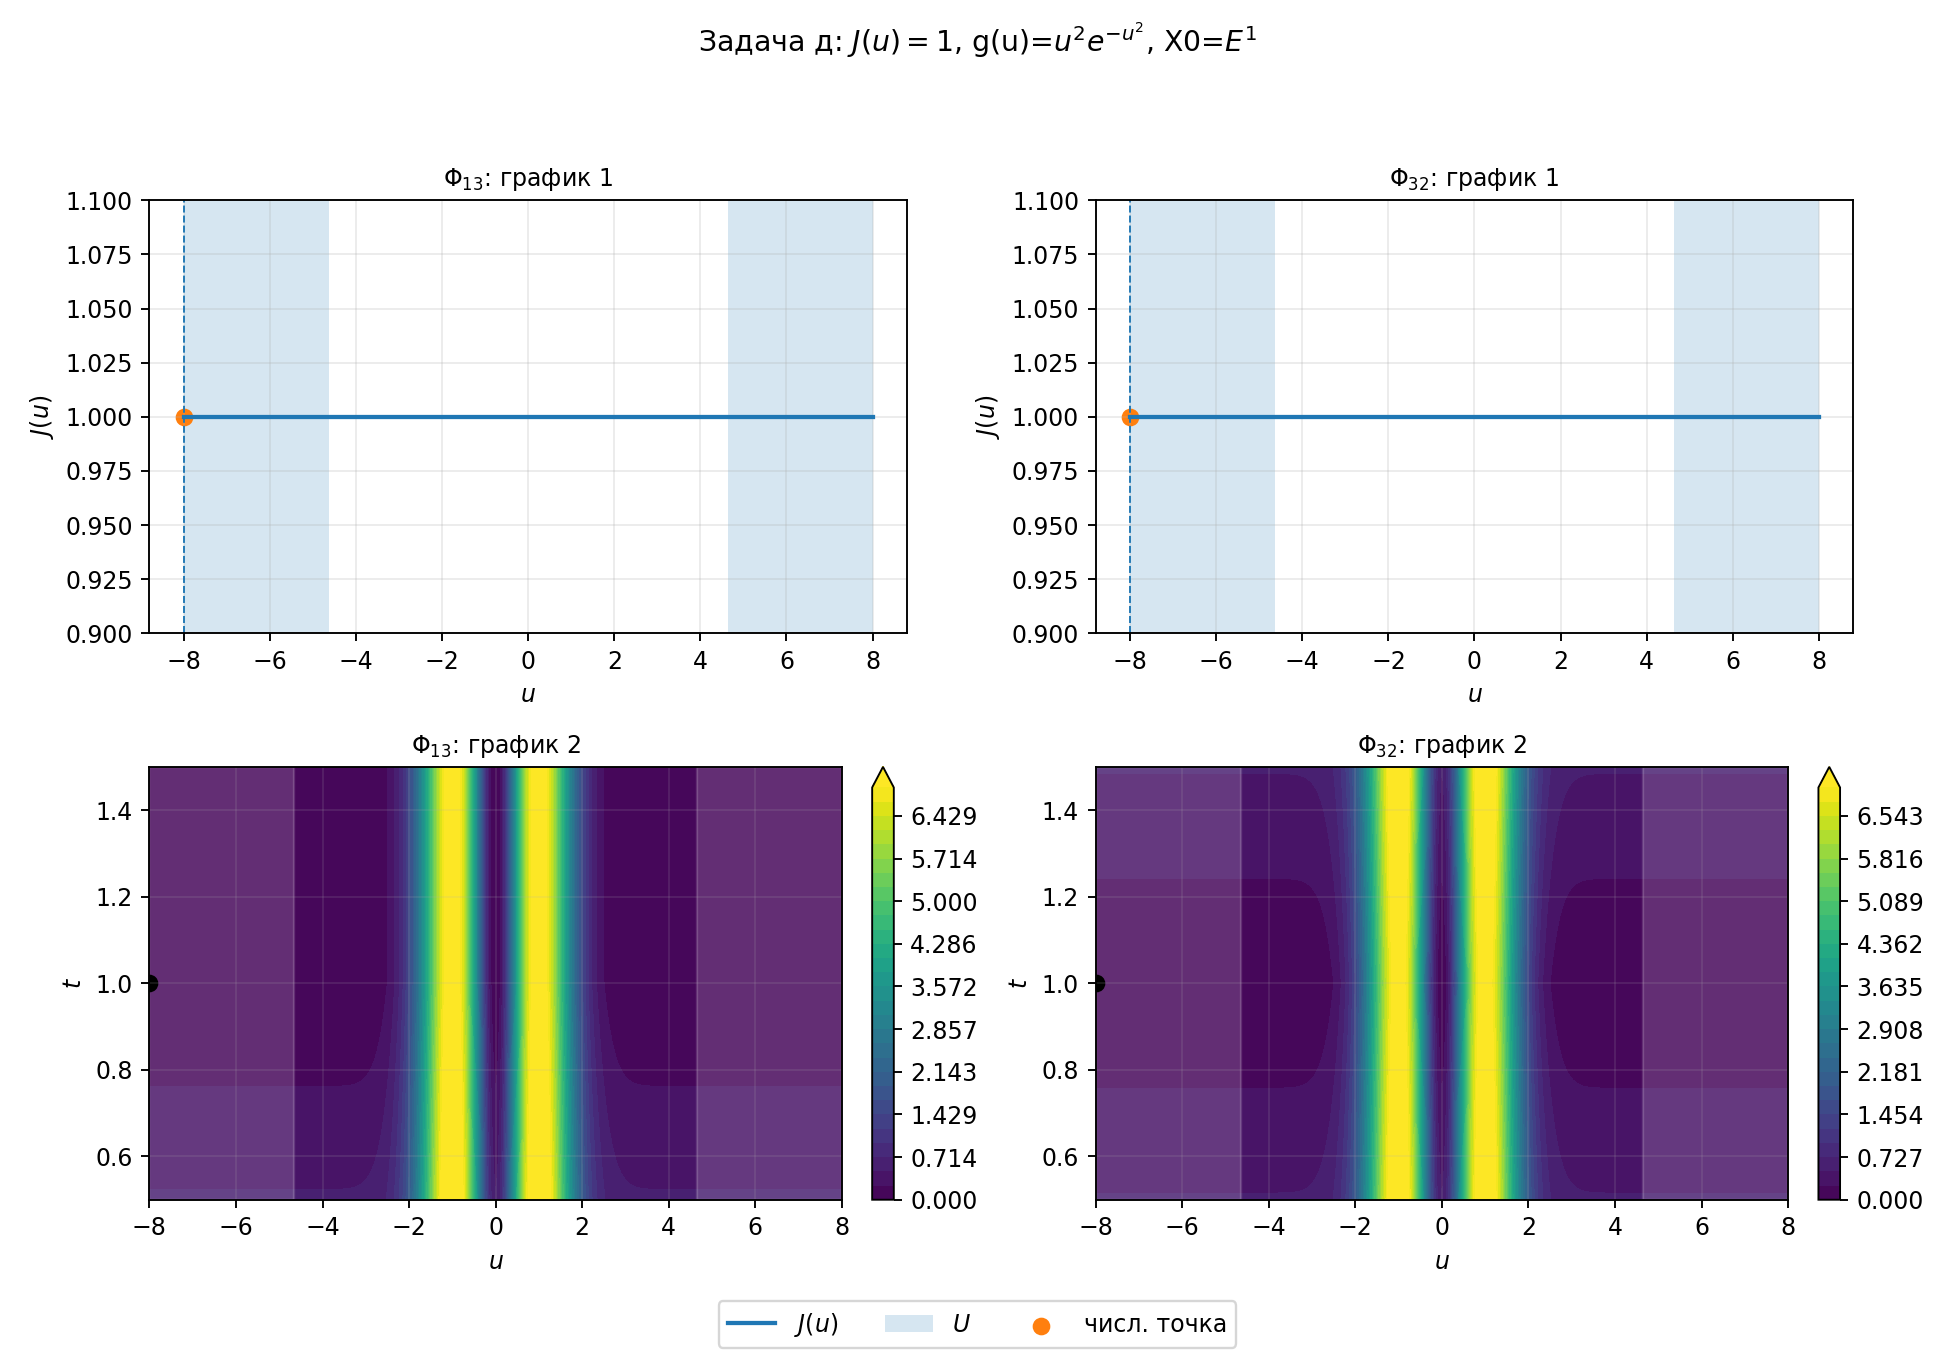
\includegraphics[width=0.96\textwidth]{graphs/d_g4_R_overview.png}
\caption{Задача д, вариант g4: $g(u)=u^2e^{-u^2}$, $X_0=E^1$. Верхний ряд: график 1 для $\Phi_{13}$ и $\Phi_{32}$; нижний ряд: график 2 для $\Phi_{13}$ и $\Phi_{32}$.}
\end{figure}

\begin{figure}[H]
\centering
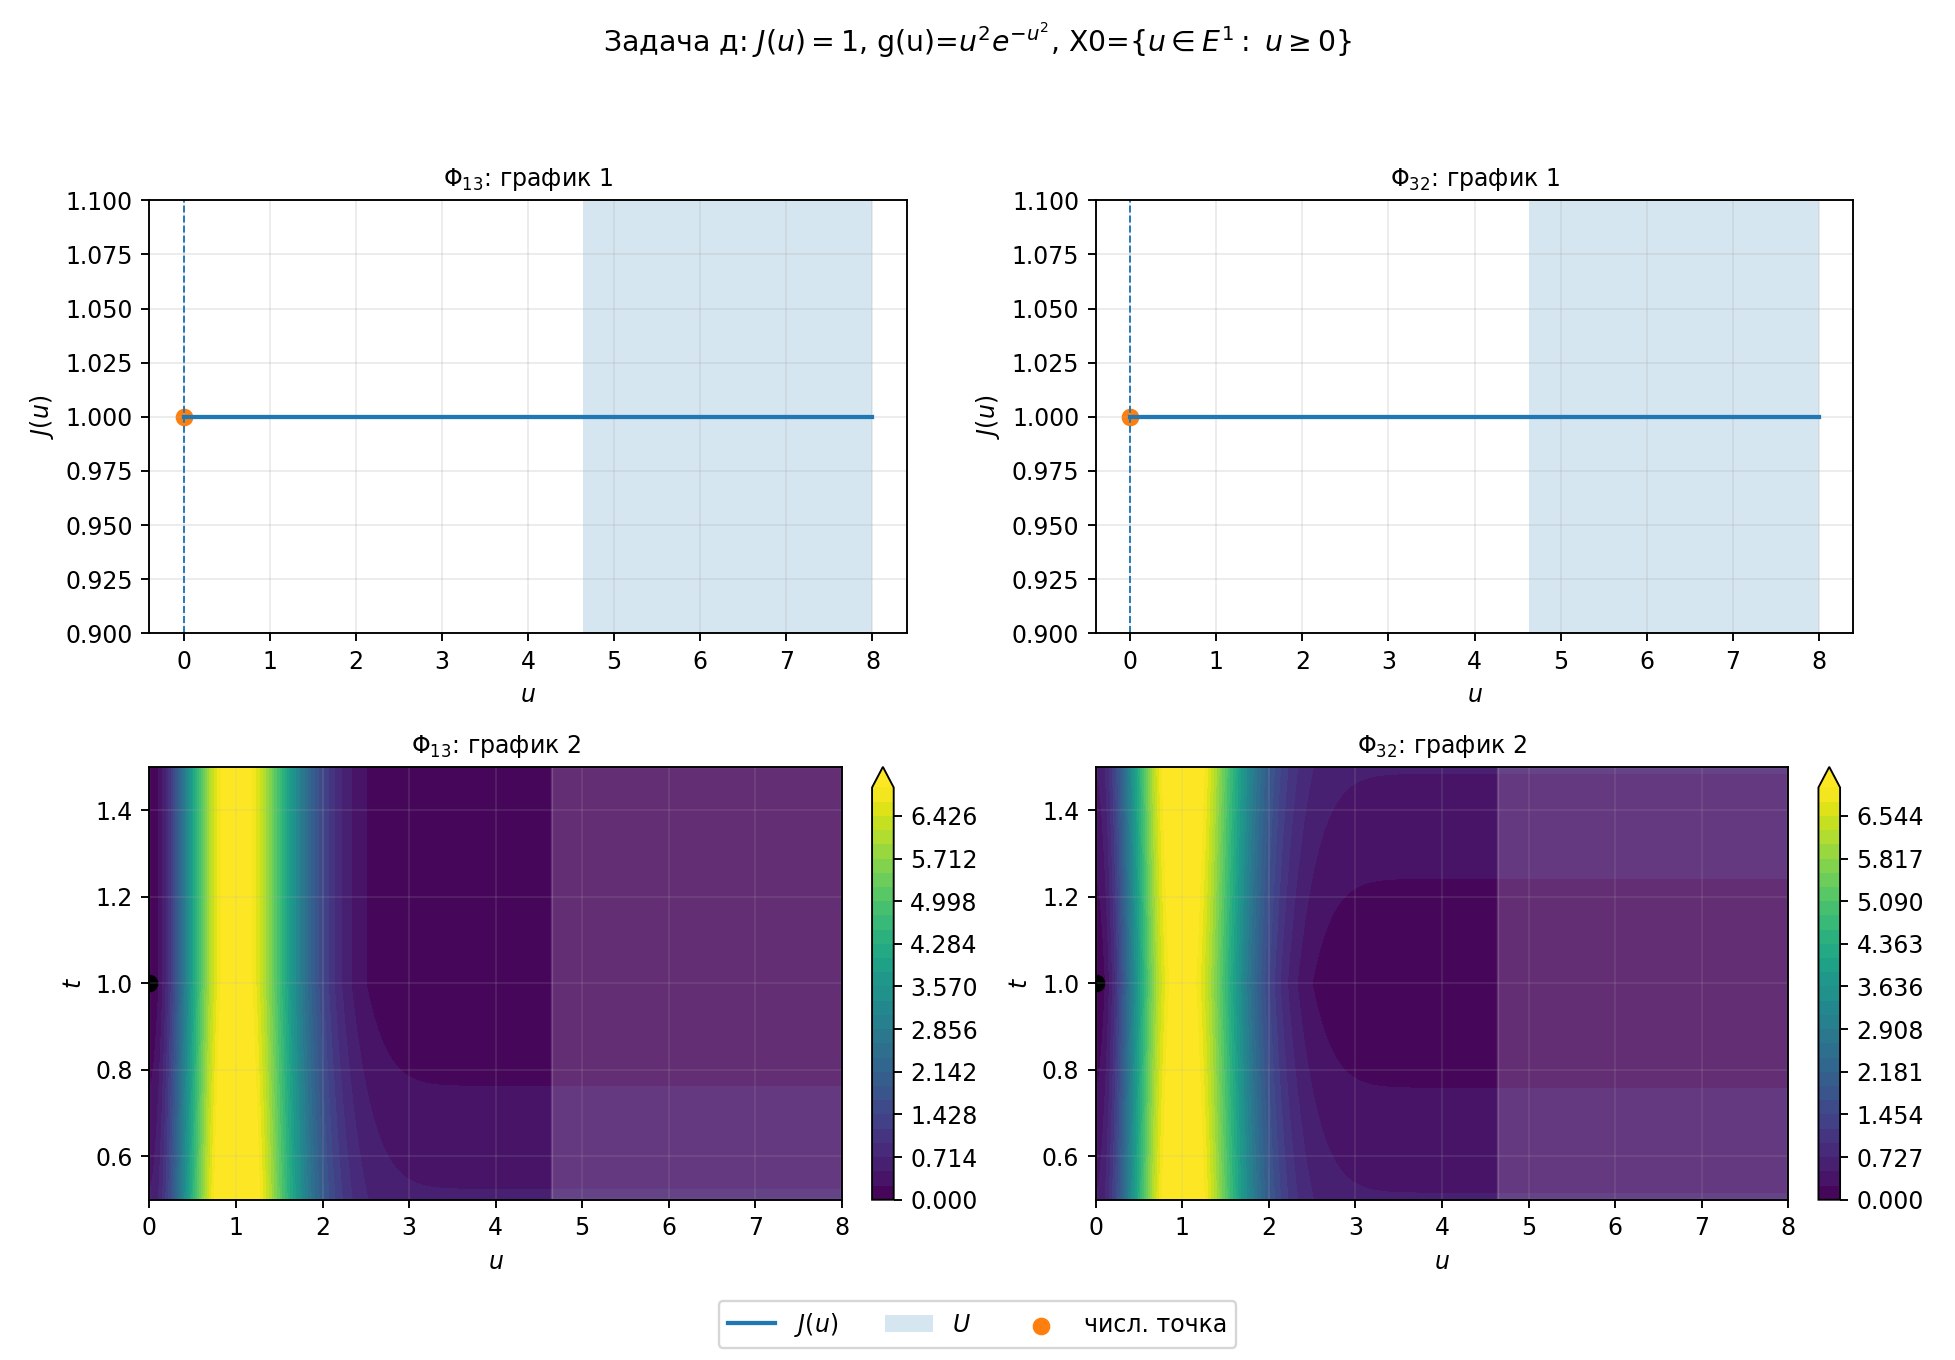
\includegraphics[width=0.96\textwidth]{graphs/d_g4_xge0_overview.png}
\caption{Задача д, вариант g4: $g(u)=u^2e^{-u^2}$, $X_0=\{u\in E^1:\ u\geq 0\}$. Верхний ряд: график 1 для $\Phi_{13}$ и $\Phi_{32}$; нижний ряд: график 2 для $\Phi_{13}$ и $\Phi_{32}$.}
\end{figure}
